% ============================================================
% MODUL 4.4 — HANDOUT DENGAN GAMBAR REFERENSI
% ============================================================
% CARA PENGGUNAAN:
% 1. Buat subfolder "gambar/" di satu folder dengan file .tex ini
% 2. Unduh semua gambar dari URL yang tercantum di komentar
%    di atas setiap \includegraphics, simpan dengan nama file
%    yang sesuai (nama file sudah ada di \includegraphics)
% 3. Kompilasi: pdflatex modul44_handout_with_figures.tex
%
% Catatan: Untuk file SVG, konversi dulu ke PNG dengan Inkscape
%   atau gunakan xelatex/lualatex + \usepackage{svg}
% ============================================================

\pdfminorversion=7
\documentclass[12pt,a4paper]{report}
\usepackage[bahasa]{babel}
\usepackage[utf8]{inputenc}
\usepackage[T1]{fontenc}
\usepackage{geometry}
\geometry{a4paper, margin=2.5cm, top=3cm, bottom=2.5cm, footskip=1.5cm}
\usepackage{xcolor}
\usepackage[most]{tcolorbox}
\usepackage{booktabs}
\usepackage{longtable}
\usepackage{tabularx}
\usepackage{xltabular}
\usepackage{enumitem}
\usepackage{lmodern}
\usepackage{microtype}
\usepackage{titlesec}
\usepackage{fancyhdr}
\usepackage{hyperref}
\usepackage{graphicx}
\usepackage{array}
\usepackage{colortbl}
\usepackage{float}
\usepackage{wrapfig}
\usepackage{caption}
\usepackage{amssymb}
\usepackage{tikz}
\usetikzlibrary{arrows.meta, positioning, shapes.geometric, calc, backgrounds, fit, decorations.markings}
\graphicspath{{gambar/}}

% ---------- background template handout ----------
\usepackage{eso-pic}
\newcommand{\switchtocontentbg}{%
  \ClearShipoutPictureBG%
  \AddToShipoutPictureBG{%
    \AtPageLowerLeft{%
      
\includegraphics[width=\paperwidth,height=\paperheight]{template-handout/content_handout.png}%
    }%
  }%
}

% Warna tambahan untuk tabel
\definecolor{rowalt}{RGB}{235,243,250}
\definecolor{rowhead}{RGB}{0,75,135}
\newcolumntype{Y}{>{\centering\arraybackslash}X}
\newcolumntype{P}[1]{>{\centering\arraybackslash}p{#1}}

\definecolor{plnblue}{RGB}{0,75,135}
\definecolor{plnorange}{RGB}{255,107,53}

\pagestyle{fancy}
\fancyhf{}
\fancyhead[L]{\scriptsize\textbf{Handout Modul 4.4 -- Keamanan \& Keterlacakan Terintegrasi}}
\fancyhead[R]{\scriptsize Level 4 (Mastery) -- PT PLN (Persero)}
\fancyfoot[C]{\small\thepage}
\renewcommand{\headrulewidth}{0.4pt}
\renewcommand{\footrulewidth}{0pt}

\titleformat{\chapter}[display]{\normalfont\huge\bfseries\color{plnblue}}{\chaptertitlename\ \thechapter}{20pt}{\Huge}
\titleformat{\section}{\Large\bfseries\color{plnblue}}{\thesection}{1em}{}
\titleformat{\subsection}{\large\bfseries\color{plnblue}}{\thesubsection}{1em}{}
\titlespacing*{\chapter}{0pt}{-30pt}{20pt}
\titlespacing*{\section}{0pt}{12pt}{8pt}
\titlespacing*{\subsection}{0pt}{10pt}{6pt}

\newtcolorbox{plnbox}[1][]{colback=plnblue!5!white, colframe=plnblue, fonttitle=\bfseries, title=#1, sharp corners, boxrule=0.8pt, breakable}
\newtcolorbox{outputbox}{colback=green!10, colframe=green!50!black, fonttitle=\bfseries, title=Output Portofolio, sharp corners, breakable}

\setlist[itemize]{leftmargin=*, topsep=3pt, itemsep=3pt}
\setlist[enumerate]{leftmargin=*, topsep=3pt, itemsep=3pt}

\hypersetup{colorlinks=true, linkcolor=plnblue, urlcolor=plnblue, citecolor=plnblue}

\usepackage{needspace}

% ---------- cegah widow/orphan line ----------
\widowpenalty=10000
\clubpenalty=10000

\raggedbottom

\begin{document}

% ============================================================
%  HALAMAN 1: COVER dengan background template
% ============================================================
\begin{titlepage}
\thispagestyle{empty}
\AddToShipoutPictureBG*{%
  \AtPageLowerLeft{%
    
\includegraphics[width=\paperwidth,height=\paperheight]{template-handout/cover_handout.png}%
  }%
}

\begin{tikzpicture}[remember picture, overlay]
  %--- LEVEL MANEJERIAL ---
  \node[anchor=north west, text width=0.80\paperwidth, align=left]
    at ([xshift=20mm, yshift=-0.27\paperheight]current page.north west)
    {%
      {\fontsize{14pt}{18pt}\selectfont\bfseries\color{plnblue}%
       LEVEL 4 (MASTERY) -- MANAJEMEN ATAS}%
    };

  %--- Judul Utama ---
  \node[anchor=north west, text width=0.80\paperwidth, align=left]
    at ([xshift=20mm, yshift=-0.33\paperheight]current page.north west)
    {%
      {\fontsize{16pt}{20pt}\selectfont\bfseries\color{plnblue}%
       MODUL 4.4: PERANCANGAN SISTEM KEAMANAN\\[4pt]%
       \& KETERLACAKAN TERINTEGRASI}%
    };

  %--- Teks bawah ---
  \node[anchor=north west, text width=0.80\paperwidth, align=left]
    at ([xshift=20mm, yshift=-0.76\paperheight]current page.north west)
    {%
      {\fontsize{14pt}{18pt}\selectfont\bfseries\color{plnblue}%
       PUSAT PENDIDIKAN DAN PELATIHAN\\[4pt]%
       PT PLN (PERSERO)}%
    };
\end{tikzpicture}
\end{titlepage}

\switchtocontentbg

\begin{center}
{\Large\bfseries\color{plnblue} Petunjuk Penggunaan Handout}\\[0.5cm]
\end{center}

\begin{plnbox}[Ikon \& Konvensi Visual]
Handout ini menggunakan beberapa konvensi visual untuk memudahkan navigasi:
\begin{itemize}[leftmargin=*]
    \item \textbf{Boks biru} seperti ini berisi ringkasan strategis, panduan tata kelola, atau template kebijakan yang menjadi perhatian utama Manajemen Atas.
    \item \textbf{Boks hijau} berjudul ``Output Portofolio'' menandakan tugas yang harus dikerjakan dan dikumpulkan sebagai bukti kompetensi.
    \item \textbf{Tabel} menyajikan matriks, rubrik penilaian, dan data terstruktur -- gunakan sebagai referensi.
    \item \textbf{Diagram/gambar} mengilustrasikan konsep kunci -- setiap diagram disertai caption multi-baris dengan penjelasan dan sumber.
    \item \textbf{Catatan kaki} berisi sitasi regulasi dan standar.
\end{itemize}
\end{plnbox}

\begin{plnbox}[Cara Menggunakan Handout Ini]
\begin{enumerate}[leftmargin=*]
    \item \textbf{Sebelum pelatihan:} Baca Pendahuluan untuk memahami konteks, target kompetensi, dan arsitektur keamanan terintegrasi. Gunakan Glosarium di akhir dokumen sebagai referensi istilah teknis.
    \item \textbf{Saat pelatihan:} Durasi fasilitasi 45 menit (Pendahuluan 5$\cdot$ RBAC 10$\cdot$ Audit 10$\cdot$ ISMS 10$\cdot$ DR 7$\cdot$ Kasus 3). Kerjakan Aktivitas Workshop di setiap bab secara mandiri (30 menit/bab). Hasil workshop menjadi bagian dari Portofolio yang dinilai.
    \item \textbf{Studi kasus:} Bab 5 menguji pemahaman holistik -- baca skenario kebocoran arsip kontrak dan analisis dari 4 perspektif pilar keamanan.
    \item \textbf{Setelah pelatihan:} Lihat Bab 6 (Validasi \& Rubrik Penilaian) untuk memahami kriteria kelulusan dan menyusun komitmen tindak lanjut.
\end{enumerate}
\end{plnbox}

\vspace{0.5cm}
\noindent\small\textit{Catatan: Seluruh materi dalam handout ini dirancang agar dapat dipahami secara mandiri oleh Manajemen Atas. Istilah teknis yang belum familiar dapat ditemukan di Glosarium di bagian akhir dokumen.}

\tableofcontents

\chapter*{Pendahuluan}
\addcontentsline{toc}{chapter}{Pendahuluan}
% Penomeran section Pendahuluan: A, B, C, D
\setcounter{section}{0}
\renewcommand{\thesection}{\Alph{section}}
Modul 4.4 merupakan mata pelajaran penutup dalam Level 4 (Mastery) yang berfokus pada perancangan tata kelola keamanan, integritas, dan keterlacakan arsip digital. Sasaran utamanya adalah membekali Manajemen Atas PLN dengan kemampuan merancang sistem keamanan yang terintegrasi penuh dengan kebijakan korporasi, regulasi nasional, dan prinsip GCG BUMN.

Dua konsep kunci yang menjadi landasan modul ini perlu dipahami sejak awal. Pertama, \textit{Aset Informasi Kritis} adalah informasi yang kehilangan, kerusakan, atau pengungkapannya dapat menimbulkan dampak serius terhadap kelangsungan operasional, kepatuhan regulasi, atau reputasi organisasi. Dalam konteks PLN, aset informasi kritis mencakup kontrak pembangkit, laporan keuangan teraudit, dokumen RUPS, dan data pelanggan. Kedua, \textit{Klasifikasi Arsip} adalah pengelompokan arsip berdasarkan tingkat sensitivitas dan dampak keamanannya. Modul ini menggunakan empat tingkat klasifikasi yang selaras dengan regulasi nasional dan praktik korporasi PLN: \textit{Vital} (kerusakan berdampak nasional), \textit{Rahasia} (kerusakan berdampak regional/unit), \textit{Terbatas} (kerusakan berdampak operasional terbatas), dan \textit{Publik} (tidak ada dampak signifikan).

\needspace{4\baselineskip}

\section{Konteks \& Urgensi: Mengapa Ini Penting bagi PLN?}
PLN sebagai Badan Usaha Milik Negara yang mengelola infrastruktur kelistrikan nasional menghadapi tantangan keamanan arsip digital yang semakin kompleks. Data Badan Siber dan Sandi Negara (BSSN) mencatat total anomali trafik serangan siber di Indonesia mencapai 1,63 miliar kejadian pada tahun 2021\footnote{Kompas.com, \textit{BSSN Sebut Ada 1,6 Miliar Serangan Siber Selama 2021}, 7 Maret 2022.} dan meningkat menjadi 3,64 miliar hanya dalam periode Januari--Juli 2025\footnote{Tempo.co, \textit{BSSN Catat 3,64 Miliar Serangan Siber di Indonesia Setengah Tahun Ini}, 29 Juli 2025.}, dengan BUMN menjadi salah satu target utama. Dalam konteks kearsipan, risiko ini bukan hanya soal teknis -- melainkan soal akuntabilitas hukum dan kepatuhan regulasi.

Pertimbangkan skenario berikut: jika kontrak pembangkit senilai triliunan rupiah bocor karena akses tidak terkontrol, atau jika arsip vital menghilang tanpa audit trail yang dapat mempertanggungjawabkan siapa yang mengaksesnya kapan, maka PLN menghadapi risiko ganda: (1) kerugian finansial dan operasional akibat kehilangan aset informasi kritis, serta (2) sanksi regulasi dari OJK, BPK, ANRI, dan lembaga pengawas lainnya. Dalam perspektif GCG, kegagalan menjaga keamanan dan keterlacakan arsip secara langsung memengaruhi penilaian tata kelola perusahaan -- termasuk dalam parameter TARIF yang menjadi tolok ukur kinerja BUMN.

Modul ini dirancang untuk menjawab kebutuhan tersebut dengan pendekatan empat pilar terintegrasi: Kontrol Akses (TK-1), Audit Trail (TK-2), Kebijakan Keamanan (TK-3), dan Backup/Disaster Recovery (TK-4). Studi kasus nyata di Bab 5 akan mendemonstrasikan bagaimana kegagalan pada satu pilar dapat menyebabkan kerentanan sistemik yang berdampak langsung pada operasional dan reputasi PLN.

\needspace{4\baselineskip}

\section{Target Kompetensi}
Setelah menyelesaikan modul ini, peserta diharapkan mampu mencapai empat kompetensi utama yang dipetakan terhadap kriteria penilaian sebagai berikut:

\begingroup
\small
\begin{xltabular}{\textwidth}{@{} c X l @{}}
\caption{Pemetaan Target Kompetensi terhadap Kriteria Penilaian}\\
\toprule
\textbf{Kode} & \textbf{Target Kompetensi} & \textbf{Kriteria Penilaian} \\
\midrule
\endfirsthead

\multicolumn{3}{@{}l}{\small\textit{Lanjutan Tabel \thetable}}\\
\toprule
\textbf{Kode} & \textbf{Target Kompetensi} & \textbf{Kriteria Penilaian} \\
\midrule
\endhead

\bottomrule
\endfoot

TK-1 & Peserta mampu merancang skema kontrol akses terintegrasi berbasis peran (RBAC) yang menghubungkan sistem kearsipan dengan sistem kepegawaian. & 4.4.1 \\
TK-2 & Peserta mampu merancang mekanisme audit trail otomatis yang merekam setiap akses dan perubahan arsip. & 4.4.2 \\
TK-3 & Peserta mampu merumuskan kebijakan keamanan yang terintegrasi dengan sistem manajemen keamanan informasi organisasi. & 4.4.3 \\
TK-4 & Peserta mampu merancang sistem backup dan disaster recovery terintegrasi. & 4.4.4 \\
\end{xltabular}
\endgroup

Keempat target kompetensi di atas bersifat kumulatif dan terintegrasi: keberhasilan pencapaian pada setiap kompetensi menjadi prasyarat efektivitas kompetensi berikutnya. Misalnya, skema RBAC yang dirancang pada TK-1 akan menentukan siapa yang tercatat dalam audit trail (TK-2), yang pada gilirannya menjadi input kebijakan keamanan (TK-3) dan memengaruhi prioritas backup (TK-4).

\needspace{4\baselineskip}

\section{Sasaran \& Prasyarat Peserta}
\begin{itemize}[leftmargin=*]
    \item Target: Manajemen Atas (Unit Kearsipan, IT Governance, GCG, Risk Management)
    \item Prasyarat: Lulus Modul 4.3, memahami klasifikasi arsip dasar, familiar dengan sistem SAP (sistem perencanaan sumber daya perusahaan) dan \textit{Single Sign-On} (SSO) organisasi
    \item Output: 4 dokumen portofolio kebijakan/prosedur siap validasi manajemen, masing-masing membuktikan pencapaian TK-1 hingga TK-4
\end{itemize}

\noindent Modul 4.4 berdiri di atas fondasi yang dibangun oleh tiga modul sebelumnya dalam Level 4. Tabel \ref{tab:ringkasan-modul} merangkum cakupan masing-masing modul dan kaitannya dengan Modul 4.4:

\begingroup
\small
\begin{xltabular}{\textwidth}{@{} >{\raggedright\arraybackslash}p{1.5cm} X X @{}}
\caption{Ringkasan Modul 4.1--4.3 dan Kaitannya dengan Modul 4.4}
\label{tab:ringkasan-modul}\\
\toprule
\textbf{Modul} & \textbf{Judul \& Cakupan Utama} & \textbf{Relevansi dengan Modul 4.4} \\
\midrule
\endfirsthead

\multicolumn{3}{@{}l}{\small\textit{Lanjutan Tabel \thetable}}\\
\toprule
\textbf{Modul} & \textbf{Judul \& Cakupan Utama} & \textbf{Relevansi dengan Modul 4.4} \\
\midrule
\endhead

\bottomrule
\endfoot

\rowcolor{rowalt}
4.1 & Merancang Potensi Integrasi Sistem, Prosedur, dan Teknologi Kearsipan Eksisting. Peserta mampu merancang peta kondisi eksisting, matriks potensi integrasi, dan skenario integrasi terpadu. & Menyediakan pemetaan aset dan sistem yang menjadi objek perlindungan keamanan dalam Modul 4.4. \\
\rowcolor{white}
4.2 & Perancangan Arsitektur Sistem Terintegrasi. Peserta mampu merancang diagram arsitektur, titik integrasi antar subsistem (penciptaan, penggunaan, pemeliharaan, penyusutan), dan spesifikasi teknis/fungsional. & Menyediakan arsitektur sistem yang menjadi infrastruktur bagi kontrol keamanan (RBAC, audit trail) dalam Modul 4.4. \\
\rowcolor{rowalt}
4.3 & Optimalisasi Prosedur dan Alur Kerja Terintegrasi. Peserta mampu mengevaluasi prosedur eksisting, merancang alur kerja baru, dan menganalisis potensi peningkatan efektivitas. & Menyediakan prosedur dan alur kerja operasional yang harus dilindungi oleh kebijakan keamanan dalam Modul 4.4. \\
\end{xltabular}
\endgroup

\noindent Ketiga modul tersebut menjadi prasyarat karena Modul 4.4 tidak membahas desain arsitektur teknis (ranah 4.2) atau optimalisasi alur kerja bisnis (ranah 4.3) secara langsung, melainkan berfokus pada lapisan tata kelola keamanan yang memastikan arsip digital PLN terlindungi, terlacak, dan tersedia.

\needspace{4\baselineskip}

\section{Arsitektur Keamanan Terintegrasi}
Keempat target kompetensi dalam modul ini tidak berdiri sendiri, melainkan membentuk satu sistem tata kelola keamanan arsip yang saling terkait. Pemahaman terhadap hubungan antar-TK menjadi kunci bagi Manajemen Atas untuk mengarahkan tim secara koheren dan menghindari solusi parsial yang tidak saling mendukung.

\begingroup
\small
\begin{xltabular}{\textwidth}{@{} l l X @{}}
\caption{Hubungan Terintegrasi antar Target Kompetensi}\\
\toprule
\textbf{TK} & \textbf{Terhubung dengan} & \textbf{Bentuk Integrasi} \\
\midrule
\endfirsthead

\multicolumn{3}{@{}l}{\small\textit{Lanjutan Tabel \thetable}}\\
\toprule
\textbf{TK} & \textbf{Terhubung dengan} & \textbf{Bentuk Integrasi} \\
\midrule
\endhead

\bottomrule
\endfoot

TK-1 (RBAC) & TK-2, TK-3 & Matriks peran menentukan WHO yang tercatat di audit trail (TK-2) dan menjadi input penetapan kewenangan dalam kebijakan (TK-3). \\
TK-2 (Audit Trail) & TK-1, TK-3, TK-4 & Log audit membuktikan kepatuhan RBAC (TK-1), menjadi bukti kepatuhan ISMS (TK-3), dan log operasi backup sendiri harus di-audit (TK-4). \\
TK-3 (Kebijakan ISMS) & TK-1, TK-2, TK-4 & Kebijakan menjadi payung hukum bagi RBAC (TK-1), menetapkan standar audit (TK-2), dan menentukan kebijakan retensi/recovery (TK-4). \\
TK-4 (Backup/DR) & TK-2, TK-3 & Backup melindungi log audit trail (TK-2) dan merupakan kontrol wajib dalam kerangka ISMS (TK-3). \\
\end{xltabular}
\endgroup

\begin{plnbox}[Pandangan Strategis untuk Manajemen Atas]
Ketika mengesahkan kebijakan keamanan arsip, Manajemen Atas harus memastikan bahwa keempat pilar ini dirancang secara bersamaan, bukan secara berurutan oleh unit yang berbeda tanpa koordinasi. Solusi parsial -- misalnya implementasi RBAC tanpa audit trail, atau backup tanpa kebijakan retensi -- akan menciptakan celah keamanan yang tidak terdeteksi hingga terjadi insiden. Studi kasus di Bab 5 akan mendemonstrasikan bagaimana keempat pilar ini saling bergantung dalam situasi nyata.
\end{plnbox}

%% ============================================================
%% GAMBAR 0.1 — KERANGKA BERPIKIR MODUL 4.4
%% Versi terbaru: gambar/kerangka_pikir.png (draw.io export)
%% Diagram konseptual yang menunjukkan bagaimana materi
%% disusun untuk memenuhi seluruh target/kriteria penilaian
%% ============================================================

\begin{figure}[H]
\centering
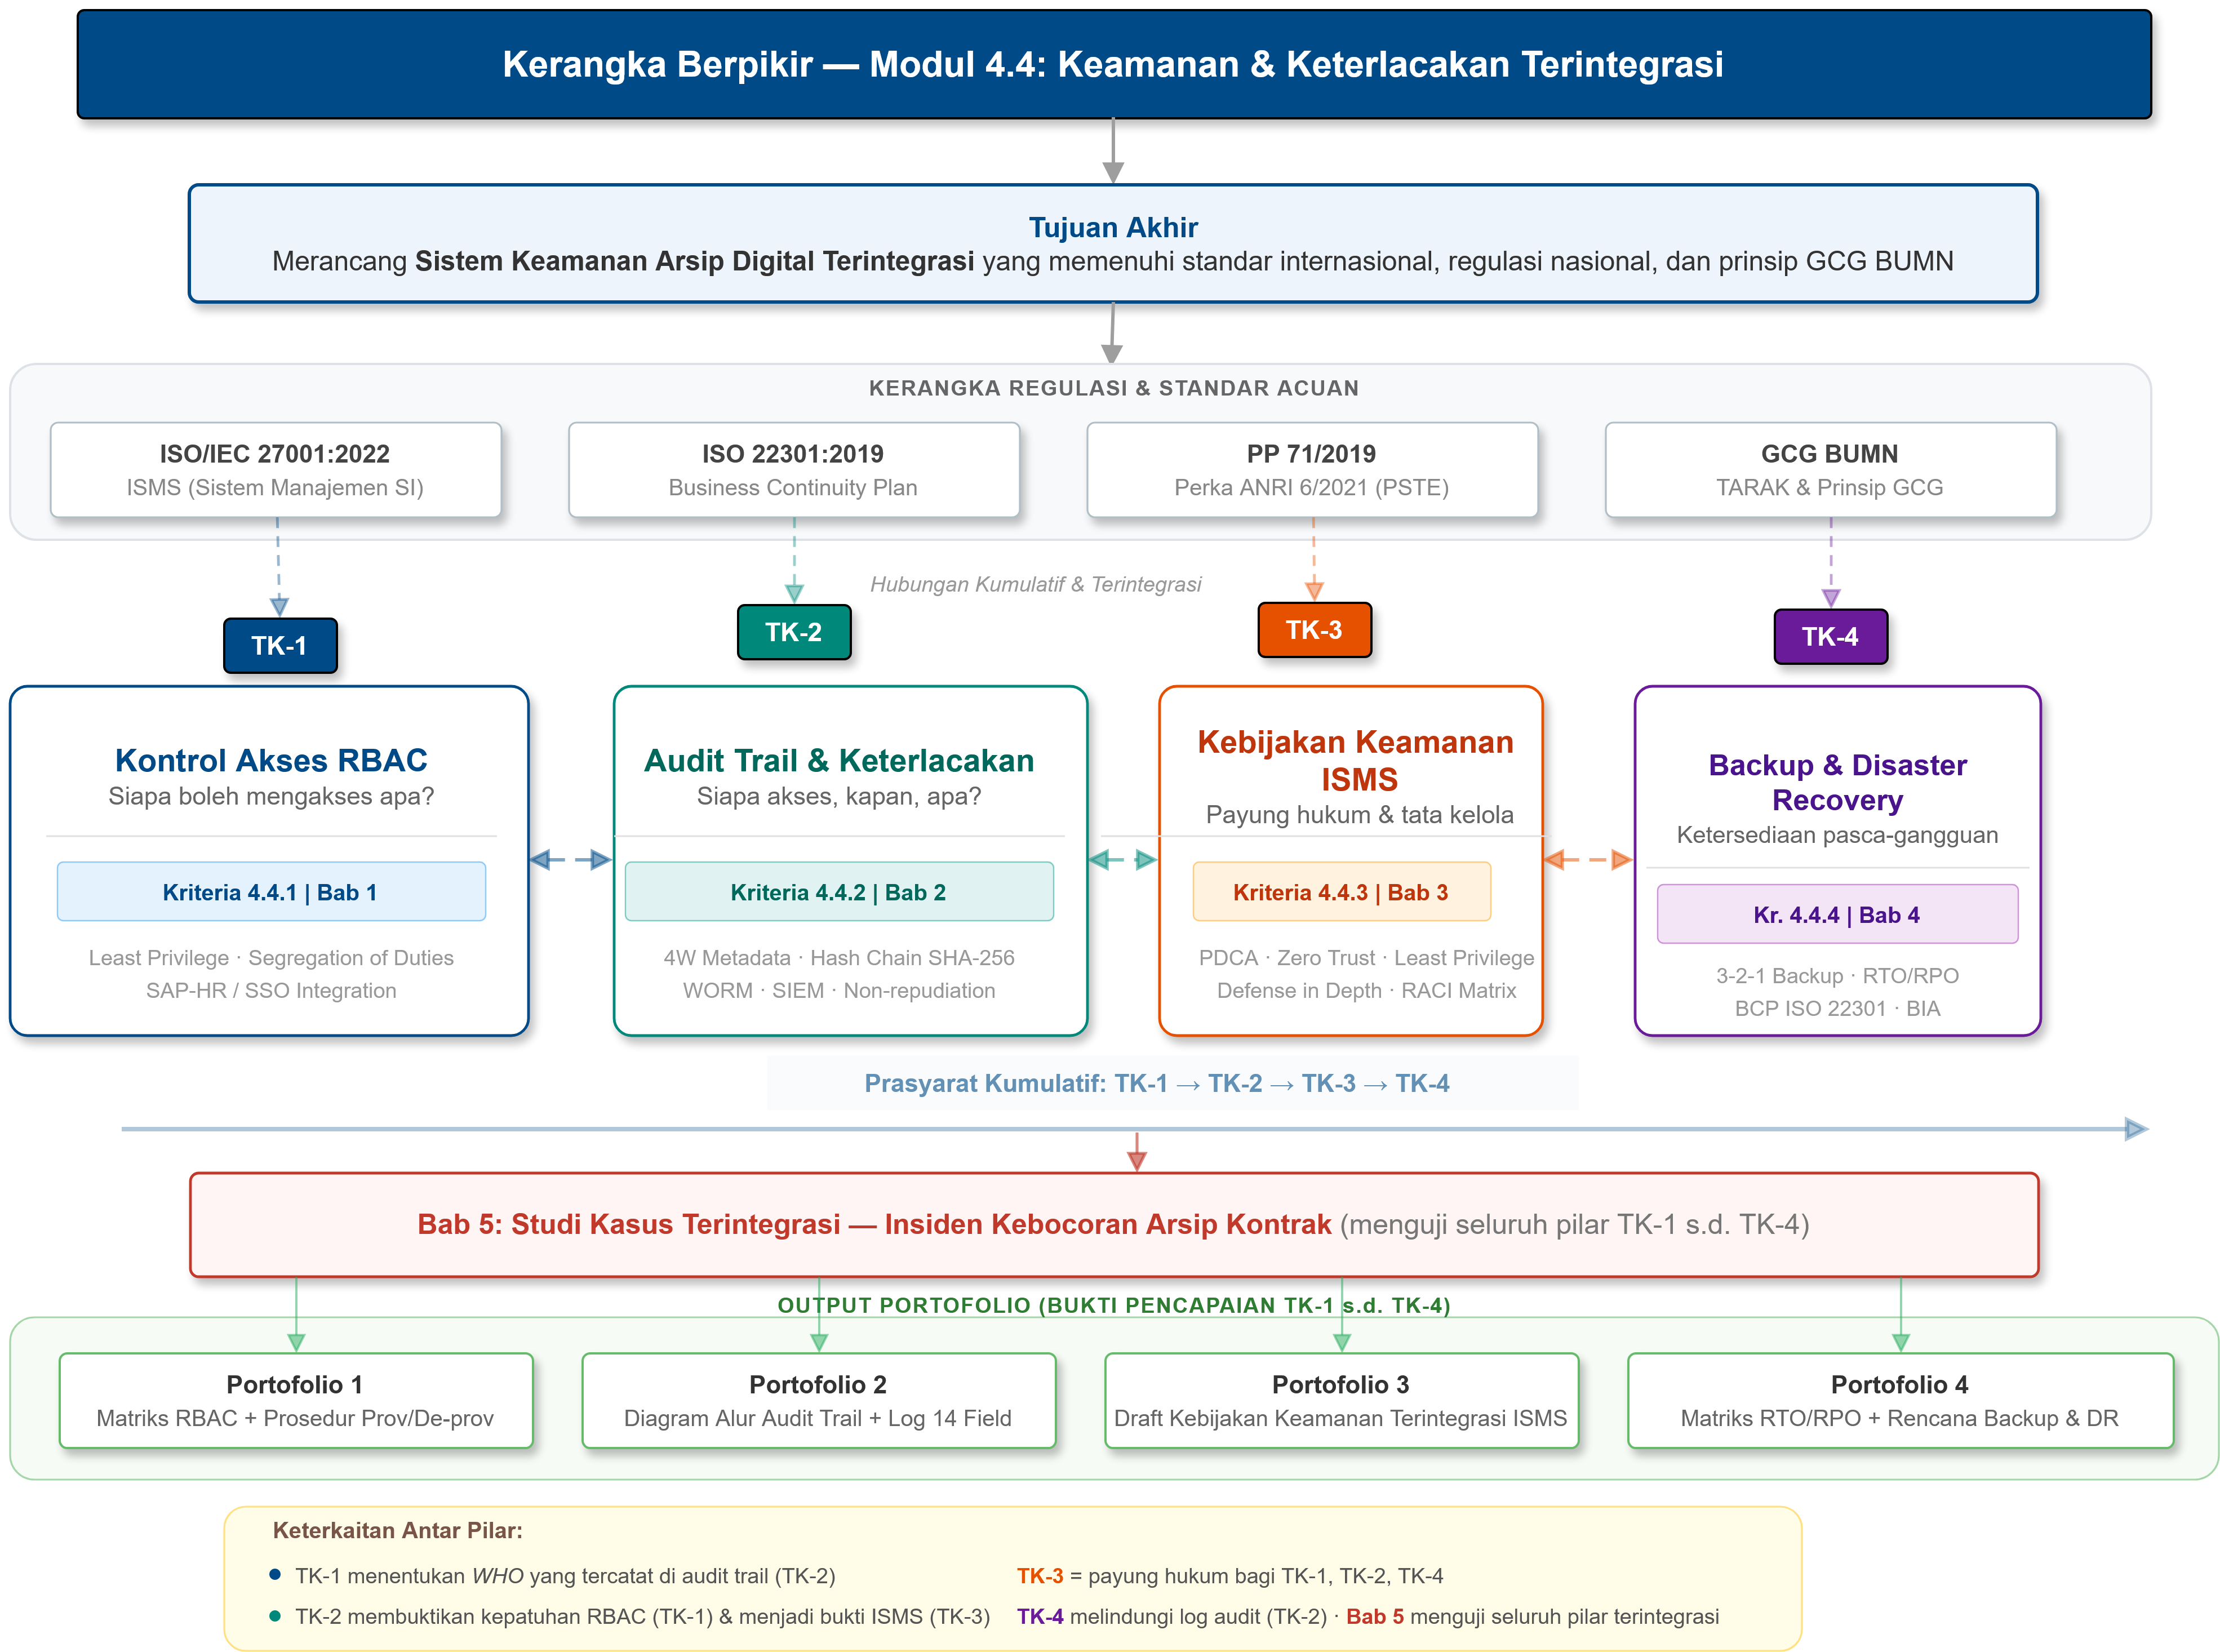
\includegraphics[width=1.0\textwidth]{gambar/kerangka_pikir.png}
\caption{Kerangka Berpikir Modul 4.4 -- Pemetaan empat pilar kompetensi terhadap kriteria penilaian}
\label{fig:kerangka-berpikir}
\end{figure}

\small Gambar \ref{fig:kerangka-berpikir} merupakan peta jalan yang menjawab pertanyaan sentral: ``Bagaimana materi Modul 4.4 disusun sehingga mampu memenuhi seluruh target kompetensi dan kriteria penilaian?'' Diagram ini menunjukkan bahwa modul ini dirancang dengan pendekatan empat pilar kumulatif: (1) TK-1 (Bab 1) -- Kontrol Akses RBAC yang menjawab pertanyaan siapa yang boleh mengakses arsip; (2) TK-2 (Bab 2) -- Audit Trail yang menjawab pertanyaan kapan dan apa yang dilakukan terhadap arsip; (3) TK-3 (Bab 3) -- Kebijakan Keamanan ISMS yang menjadi payung hukum bagi seluruh kontrol; dan (4) TK-4 (Bab 4) -- Backup/Disaster Recovery yang menjamin ketersediaan arsip pasca-gangguan.

Setiap pilar didukung oleh kerangka regulasi dan standar di baris atas: ISO/IEC 27001:2022 (ISMS)\footnote{ISO/IEC 27001:2022, \textit{Information Security Management Systems -- Requirements}, 3rd ed. (Geneva: ISO, 2022).}, ISO 22301:2019 (Business Continuity)\footnote{ISO 22301:2019, \textit{Business Continuity Management Systems -- Requirements}, 2nd ed. (Geneva: ISO, 2019).}, PP 71/2019\footnote{PP 71/2019, Penyelenggaraan Sistem dan Transaksi Elektronik, LNRI 196 (2019).} dan Perka ANRI 6/2021\footnote{Perka ANRI 6/2021, Pengelolaan Arsip Elektronik, BNRI 541 (2021).} (kearsipan nasional), serta prinsip GCG BUMN/TARIF\footnote{Permen BUMN PER-2/MBU/03/2023, Pedoman GCG Signifikan BUMN, BNRI 274 (2023).}. Garis penghubung antar-pilar menunjukkan bahwa keempat pilar bersifat kumulatif -- keberhasilan pada pilar sebelumnya menjadi prasyarat efektivitas pilar berikutnya. Bab 5 (Studi Kasus) di bagian bawah menjadi titik integrasi yang menguji apakah peserta mampu menerapkan seluruh pilar secara sinergis dalam situasi insiden nyata. Keempat Portofolio di baris paling bawah merupakan bukti pencapaian kompetensi yang menjadi dasar penilaian.

% ============================================================
% Kembalikan penomeran section ke format 1.1, 2.1, ...
\renewcommand{\thesection}{\thechapter.\arabic{section}}
\chapter{Kontrol Akses Berbasis Peran (RBAC) Terintegrasi}
(Kriteria Penilaian 4.4.1)
% ============================================================

Bab ini mendukung pencapaian Pilar 1: Kontrol Akses -- peserta mampu merancang skema kontrol akses terintegrasi berbasis peran (RBAC) yang menghubungkan sistem kearsipan dengan sistem kepegawaian. RBAC bukan sekadar matriks izin, melainkan kerangka tata kelola yang menghubungkan identitas kepegawaian dengan hak akses arsip secara otomatis. Tiga prinsip fundamental yang mendasari RBAC perlu dipahami oleh Manajemen Atas:

\textit{Least Privilege} (hak akses minimum) adalah prinsip yang menyatakan bahwa setiap pengguna atau sistem hanya boleh diberikan hak akses yang benar-benar diperlukan untuk menjalankan tugasnya -- tidak lebih. Dalam konteks kearsipan PLN, prinsip ini berarti bahwa staf administrasi tidak perlu memiliki hak Ekspor terhadap arsip Rahasia jika tugasnya hanya memerlukan hak Read. Penerapan \textit{least privilege} meminimalkan luasnya dampak jika terjadi insiden keamanan, karena penyerang atau pengguna yang kompromikan hanya memiliki akses terbatas.

\textit{Segregation of Duties} (pemisahan fungsi) adalah prinsip yang memastikan tidak ada satu peran yang memiliki kombinasi hak akses yang berlebihan sehingga menciptakan potensi konflik kepentingan atau celah pengawasan. Dalam kearsipan, ini berarti pemisahan antara hak membuat arsip (Create), menyetujui arsip (Approve), dan mengekspor arsip (Export) ke peran yang berbeda. Tanpa \textit{segregation of duties}, satu orang dapat secara mandiri menciptakan, menyetujui, dan mengekspor dokumen tanpa mekanisme keseimbangan pengawasan.

\textit{Prosedur Darurat} (\textit{break-glass procedure}) adalah mekanisme yang memungkinkan akses khusus di luar hak akses normal dalam situasi darurat, dengan catatan bahwa setiap penggunaan prosedur darurat dicatat secara lengkap dalam audit trail dan memerlukan persetujuan serta eskalasi pascakejadian. Dalam konteks PLN, prosedur darurat digunakan ketika arsip Vital harus diakses di luar jam kerja untuk menangani insiden kritis, dengan persetujuan atasan langsung yang terdokumentasi.

Dalam perspektif keterlacakan (traceability), RBAC memainkan peran fundamental: tanpa kontrol akses yang terstruktur, tidak mungkin menjamin bahwa setiap jejak digital dalam audit trail benar-benar merepresentasikan tindakan pihak yang berwenang. RBAC menjadi prasyarat kredibilitas audit trail -- sebuah log yang mencatat aktivitas ``Admin Sistem'' jauh kurang bermakna dibandingkan log yang mencatat ``Budi Santoso (Kabag TU, NIP 198503152010011001) mengunduh Kontrak Pembangkit X''.

%% ============================================================
%% GAMBAR 1.1 — Model RBAC NIST
%% Unduh: https://upload.wikimedia.org/wikipedia/commons/c/c2/Role-based_access_control.svg
%% Simpan sebagai: gambar/Role-based_access_control.svg
%% (Jika SVG bermasalah, konversi ke PNG dengan Inkscape)
%% ============================================================

\begin{figure}[H]
\centering
\resizebox{0.7\textwidth}{!}{%
\begin{tikzpicture}[
  box/.style={draw=plnblue, fill=plnblue!5, rounded corners=4pt,
    line width=0.8pt, minimum width=2.8cm, minimum height=1.4cm,
    font=\small, align=center},
  arr/.style={-{Stealth[length=5pt]}, line width=0.7pt, plnblue},
  lbl/.style={font=\tiny, fill=white, inner sep=2pt, text=plnblue!80!black}
]
\node[box] (users) at (0,3) {\textbf{USERS}\\[-1pt]{\scriptsize Pengguna PLN}};
\node[box] (roles) at (5,3) {\textbf{ROLES}\\[-1pt]{\scriptsize Jabatan / Peran}};
\node[box] (perms) at (10,3) {\textbf{PERMISSIONS}\\[-1pt]{\scriptsize Hak Akses}};
\node[box] (sess)  at (2.5,0) {\textbf{SESSIONS}\\[-1pt]{\scriptsize Sesi Aktif}};
\draw[arr] (users) -- node[lbl, above]{UA} (roles);
\draw[arr] (roles) -- node[lbl, above]{PA} (perms);
\draw[arr] (users.south) -- node[lbl, left]{SC} (sess.north west);
\draw[arr] (sess.east) -- node[lbl, below, sloped]{SA} (roles.south);
\end{tikzpicture}%
}% end resizebox
\caption{Model RBAC NIST -- Komponen Utama: Users, Roles, Permissions, Sessions}
\label{fig:rbac-nist-model}
\end{figure}

\small Gambar \ref{fig:rbac-nist-model} mengilustrasikan model RBAC standar NIST yang menjadi acuan utama dalam perancangan kontrol akses berbasis peran. Model ini menunjukkan bahwa hak akses tidak diberikan langsung kepada individu (users), melainkan ditetapkan pada peran (roles) yang kemudian di-assign kepada pengguna. Pendekatan ini memungkinkan pemisahan yang jelas antara identitas pengguna dan hak aksesnya, sehingga mempermudah manajemen siklus hidup akses -- mulai dari provisioning saat penugasan baru hingga de-provisioning saat mutasi atau pensiun.

\needspace{4\baselineskip}

\section{Integrasi dengan Sistem Kepegawaian}
Bagi Manajemen Atas, integrasi RBAC dengan sistem kepegawaian adalah mekanisme pengendalian risiko bisnis, bukan semata urusan teknis IT. Prinsip utamanya sederhana: ketika status kepegawaian berubah, hak akses arsip harus berubah pada saat yang sama. Jika proses mutasi, promosi, pensiun, atau pengakhiran hubungan kerja tidak tersinkron dengan sistem akses, organisasi membuka jendela risiko kebocoran data, penyalahgunaan akun, dan temuan audit kepatuhan.

Karena itu, hak akses tidak diberikan kepada individu, melainkan kepada peran (role) yang terikat pada:
\begin{itemize}[leftmargin=*]
    \item Jabatan/Fungsi: Otomatis \textit{provisioning} saat mutasi/promosi, \textit{de-provisioning} saat pensiun/resign.
    \item \textit{Single Sign-On} (SSO): Autentikasi terpusat mengurangi risiko berbagi kata sandi dan celah akses manual.
    \item \textit{Lifecycle Management}: Review hak akses berkala (minimal tahunan) untuk memastikan relevansi dengan tugas aktual.
\end{itemize}

Untuk memastikan integrasi ini benar-benar bernilai bagi organisasi, Manajemen Atas perlu menetapkan empat keputusan tata kelola berikut:
\begin{enumerate}[leftmargin=*]
  \item Sumber Kebenaran Data Kepegawaian (\textit{single source of truth}). Tetapkan sistem HR/SAP sebagai sumber data resmi untuk status pegawai, jabatan, unit, dan masa tugas. Sistem akses arsip tidak boleh menggunakan data manual terpisah.
  \item SLA perubahan hak akses. Tetapkan standar waktu layanan yang terukur, misalnya: mutasi/promosi diproses maksimal 1x24 jam; pengakhiran hubungan kerja diproses segera (\textit{same day}) dengan prioritas tinggi.
  \item Mekanisme pengecualian yang terkendali. Akses darurat (\textit{break-glass}) boleh diberikan hanya dengan persetujuan berjenjang, masa berlaku terbatas, dan kewajiban review pasca-insiden.
  \item Akuntabilitas lintas fungsi. Tetapkan pembagian tanggung jawab jelas antara HR, Unit Kearsipan, IT Governance, dan Atasan Langsung agar tidak ada area abu-abu saat terjadi insiden.
\end{enumerate}

\begingroup
\small
\begin{xltabular}{\textwidth}{@{} >{\raggedright\arraybackslash}p{3.2cm} >{\raggedright\arraybackslash}p{2.8cm} X @{}}
\caption{Indikator Kendali Integrasi RBAC--Kepegawaian untuk Dashboard Manajemen}
\label{tab:kpi-rbac-hr}\\
\toprule
\textbf{Indikator} & \textbf{Target Praktik Baik} & \textbf{Makna bagi Manajemen Atas} \\
\midrule
\endfirsthead

\multicolumn{3}{@{}l}{\small\textit{Lanjutan Tabel \thetable}}\\
\toprule
\textbf{Indikator} & \textbf{Target Praktik Baik} & \textbf{Makna bagi Manajemen Atas} \\
\midrule
\endhead

\bottomrule
\endfoot

SLA \textit{provisioning} mutasi/promosi & Maks. 1x24 jam & Menjamin pegawai baru di fungsi tertentu dapat bekerja tanpa membuka akses berlebih. \\
SLA \textit{de-provisioning} pegawai keluar & \textit{Same day} (prioritas tinggi) & Mengurangi risiko akun yatim (\textit{orphan account}) yang sering menjadi sumber kebocoran. \\
Rasio akun tidak sesuai jabatan aktif & Mendekati 0\% & Mengukur kedisiplinan sinkronisasi antara struktur organisasi dan hak akses aktual. \\
Jumlah akses darurat tanpa review & 0 kasus & Menjamin setiap pengecualian memiliki jejak keputusan dan evaluasi pascakejadian. \\
\end{xltabular}
\endgroup

Pertanyaan eksekutif yang perlu dijawab berkala: ``Apakah perubahan struktur organisasi minggu ini otomatis tercermin pada hak akses arsip, dan apakah kita memiliki bukti auditnya?'' Jika jawabannya belum konsisten ``ya'', maka integrasi belum matang dan berisiko tinggi.

\needspace{4\baselineskip}

\section{Matriks Role \texorpdfstring{$\times$}{x} Klasifikasi Arsip PLN}
Skema akses ditentukan oleh perpotongan peran organisasi dan tingkat sensitivitas arsip. Bagi Manajemen Atas, matriks ini adalah instrumen pengambilan keputusan tata kelola yang menjawab tiga pertanyaan strategis sekaligus: \textit{siapa} yang boleh melakukan aksi tertentu, \textit{pada arsip kelas apa}, dan \textit{dengan kontrol pengaman apa}. Tabel \ref{tab:matriks-rbac} menggunakan role/jabatan aktual di lingkungan PLN yang dikelompokkan berdasarkan fungsi organisasi:

\begin{itemize}[leftmargin=*]
  \item Cara membaca kolom klasifikasi: semakin ke kanan (Terbatas $\rightarrow$ Rahasia $\rightarrow$ Vital), tingkat kontrol harus semakin ketat.
  \item Cara membaca simbol hak akses: C, R, U, A, E bukan sekadar huruf operasional, tetapi representasi level risiko keputusan bisnis.
  \item Makna superskrip darurat ($^{\dagger}$): akses diperbolehkan hanya melalui mekanisme persetujuan khusus; bukan hak akses reguler harian.
\end{itemize}

\begingroup
\footnotesize
\begin{xltabular}{\textwidth}{@{} >{\raggedright\arraybackslash}p{2.8cm} Y Y Y Y @{}}
\caption{Matriks RBAC untuk Arsip Digital PLN -- Role per Fungsi Organisasi}
\label{tab:matriks-rbac}\\
\renewcommand{\arraystretch}{1.4}
\textcolor{white}{\textbf{Peran (Role) di PLN}} & \textcolor{white}{\textbf{Publik/ Internal}} & \textcolor{white}{\textbf{Terbatas}} & \textcolor{white}{\textbf{Rahasia}} & \textcolor{white}{\textbf{Vital}} \\
\midrule
\endfirsthead

\multicolumn{5}{@{}l}{\small\textit{Lanjutan Tabel \thetable}}\\
\textcolor{white}{\textbf{Peran (Role) di PLN}} & \textcolor{white}{\textbf{Publik/ Internal}} & \textcolor{white}{\textbf{Terbatas}} & \textcolor{white}{\textbf{Rahasia}} & \textcolor{white}{\textbf{Vital}} \\
\midrule
\endhead

\bottomrule
\endfoot

\multicolumn{5}{@{}l}{\cellcolor{plnblue!15}Operasional -- Unit Kearsipan \& Tata Usaha} \\
\cmidrule(l){1-5}
Staf Kearsipan/ Arsiparis & C, R & R & R$^{\dagger}$ & -- \\
Staf Administrasi/ TU & C, R & R & -- & -- \\
Kabag TU/ Kasubag Kearsipan & C, R, U & C, R, U & R, E & R \\
Kasi TLSK$^{\ddagger}$ & C, R & R, E & R$^{\dagger}$ & -- \\
\multicolumn{5}{@{}l}{\cellcolor{plnblue!15}Fungsional -- HR, Hukum, IT} \\
\cmidrule(l){1-5}
Staf HR/ Administrasi HR & C, R & R & R$^{\dagger}$ & -- \\
Staf Hukum/ Legal & C, R & C, R, U & R, E & R \\
Staf IT/ Developer, DBA & -- & R & R & R$^{\dagger}$ \\
\multicolumn{5}{@{}l}{\cellcolor{plnblue!15}Manajemen -- Pusat \& Unit Induk} \\
\cmidrule(l){1-5}
GM / SRM Unit Induk & R & R, U & R, U, A & R, U, A \\
EVP/ SVP/ VP Pusat & R & R, U & R, U, A & R, U, A \\
\multicolumn{5}{@{}l}{\cellcolor{plnblue!15}Pengawasan -- SPI, GCG, Cyber Security} \\
\cmidrule(l){1-5}
Auditor SPI/ Staf Auditor & R & R, E & R, E & R, E \\
VP Cyber Security/ IT Sec & R & R, E & R, E & R, E \\
VP Compliance/ GCG & R & R, E & R, E & R, E \\
\multicolumn{5}{@{}l}{\cellcolor{plnblue!15}Sistem -- Otomasi \& Integrasi} \\
\cmidrule(l){1-5}
Service Account (Sistem) & Auto-capture & Auto-classify & -- & -- \\
\end{xltabular}
\endgroup
Keterangan hak akses: C = Create, R = Read, U = Update, A = Approve, E = Export/Review\\
$^{\dagger}$Dengan persetujuan atasan langsung (prosedur darurat). $^{\ddagger}$Kasi Tata Laksana Surat \& Kearsipan.\\
Role berdasarkan Peraturan Direksi PT PLN (Persero) Nomor 0037.P/DIR/2022 tentang Organisasi dan Tata Kerja\footnote{PT PLN (Persero), Perdir 0037.P/DIR/2022, Organisasi dan Tata Kerja (Jakarta: PLN, 2022).} PT PLN (Persero).

Agar dapat dimanfaatkan optimal oleh Manajemen Atas, matriks pada Tabel \ref{tab:matriks-rbac} sebaiknya digunakan sebagai \textit{alat kendali rapat} bulanan, bukan hanya lampiran dokumen. Praktik yang direkomendasikan:
\begin{enumerate}[leftmargin=*]
  \item Uji konsistensi jabatan vs hak akses. Cocokkan 10--20 sampel akun aktual dari setiap fungsi dengan matriks. Jika ditemukan hak akses di luar matriks, perlakukan sebagai temuan prioritas.
  \item Uji pemisahan fungsi kritis. Pastikan tidak ada peran yang dapat melakukan rangkaian aksi berisiko tinggi secara end-to-end (misal: Create + Approve + Export pada arsip sensitif) tanpa kontrol pengimbang.
  \item Uji tren pengecualian akses. Pantau frekuensi penggunaan prosedur darurat per unit. Tren meningkat dapat menandakan desain peran yang belum tepat atau potensi penyalahgunaan.
  \item Uji keterkaitan dengan audit trail. Pastikan setiap perubahan hak akses dan setiap ekspor arsip Rahasia/Vital dapat ditelusuri pada log audit berikut persetujuannya.
\end{enumerate}

\begin{plnbox}[Panduan Pemanfaatan Matriks untuk Keputusan Manajemen]
Gunakan matriks role sebagai dasar tiga keputusan eksekutif: (1) keputusan risiko -- peran mana yang perlu diperketat atau dibatasi; (2) keputusan kepatuhan -- unit mana yang paling berpotensi menimbulkan temuan audit; dan (3) keputusan investasi -- area mana yang perlu diprioritaskan untuk otomasi IAM/SSO, pelatihan, atau penguatan kontrol. Dengan pendekatan ini, matriks tidak berhenti sebagai artefak administratif, tetapi menjadi instrumen pengendalian risiko korporasi yang aktif.
\end{plnbox}

\needspace{4\baselineskip}

\section{Langkah-Langkah Perancangan Skema RBAC}
Bagi Manajemen Atas, perancangan skema RBAC bukan berarti merancang konfigurasi teknis sistem, melainkan memastikan bahwa proses tata kelola berikut dijalankan dengan benar oleh tim terkait:

\begin{enumerate}[leftmargin=*]
    \item Inventarisasi Peran Organisasi. Tim HR/Kepegawaian menyusun daftar seluruh peran yang bersentuhan dengan arsip digital di unit kerja. Manajemen Atas memvalidasi kelengkapan daftar ini -- memastikan tidak ada peran yang terlewat.
    \item Pemetaan Aset Arsip. Unit Kearsipan mengklasifikasikan seluruh arsip digital ke dalam 4 tingkat sensitivitas (Publik, Terbatas, Rahasia, Vital). Manajemen Atas menetapkan klasifikasi untuk arsip-arsip strategis yang memerlukan keputusan tingkat atas.
    \item Penetapan Hak Akses Minimum. Tim IT Governance bersama Unit Kearsipan menentukan hak akses per peran per klasifikasi, berdasarkan prinsip \textit{least privilege}. Manajemen Atas menyetujui matriks akhir dan memastikan tidak ada konflik kepentingan.
    \item Validasi \textit{Segregation of Duties}. Manajemen Atas memastikan tidak ada satu peran yang memiliki kombinasi hak akses yang berlebihan -- misalnya, satu orang tidak boleh sekaligus membuat, menyetujui, dan mengekspor arsip vital tanpa mekanisme keseimbangan pengawasan.
    \item Penulisan Prosedur \textit{Provisioning/De-provisioning}. Tim HR dan IT menuliskan prosedur -- baik otomatis (via SAP-HR/SSO) maupun manual -- untuk pemberian dan pencabutan hak akses. Manajemen Atas menyetujui prosedur ini dan memastikan ada mekanisme penanganan kasus darurat (misal: pencabutan akses segera saat terjadi insiden).
    \item Penetapan Jadwal Review Berkala. Manajemen Atas menetapkan frekuensi review hak akses (minimal tahunan) dan menunjuk penanggung jawab pelaksanaannya. Review harus menghasilkan daftar hak akses yang dicabut atau dimodifikasi.
\end{enumerate}

Pertanyaan kunci untuk Manajemen Atas: ``Apakah setiap peran di unit ini hanya memiliki hak akses yang benar-benar diperlukan untuk menjalankan tugasnya? Dan apakah hak akses langsung dicabut saat seseorang pindah tugas, mutasi, atau pensiun -- tanpa harus menunggu ada keluhan?''

\begin{plnbox}[Ringkasan untuk Manajemen Atas -- Bab 1]
RBAC adalah fondasi keterlacakan: tanpa kontrol akses yang jelas, audit trail menjadi tidak bermakna karena tidak dapat dipastikan bahwa setiap aksi tercatat atas nama pihak yang berwenang. Tiga pesan kunci yang harus dibawa Manajemen Atas dari bab ini: (1) RBAC bukan konfigurasi IT, melainkan keputusan tata kelola tentang siapa boleh mengakses apa; (2) matriks peran harus mencakup pemisahan fungsi (\textit{segregation of duties}) agar tidak ada satu orang yang terlalu kuat; dan (3) proses provisioning/de-provisioning harus terhubung dengan siklus hidup kepegawaian melalui SAP-HR/SSO.
\end{plnbox}

\needspace{4\baselineskip}

\section{Aktivitas Workshop (30 Menit)}
\begin{enumerate}[leftmargin=*]
    \item Identifikasi 3 peran kunci di unit Anda yang bersentuhan dengan arsip.
    \item Tentukan hak akses (CRU) untuk 3 klasifikasi arsip operasional.
    \item Rancang mekanisme review dan revokasi akses tahunan.
\end{enumerate}

\begin{outputbox}
\textbf{Portofolio 1 (Pilar 1: Kontrol Akses):} Matriks RBAC Terintegrasi + Prosedur \textit{Provisioning/De-provisioning}. Dinilai berdasarkan kemampuan peserta merancang skema kontrol akses berbasis peran yang menghubungkan sistem kearsipan dengan sistem kepegawaian, kejelasan role, prinsip \textit{least privilege}, dan keterkaitan dengan siklus hidup kepegawaian.
\end{outputbox}

% ============================================================
\chapter{Mekanisme Audit Trail Otomatis \& Keterlacakan}
(Kriteria Penilaian 4.4.2 -- Target Kompetensi 2)
% ============================================================

Mengapa bab ini berurutan setelah RBAC? Skema RBAC yang dirancang pada Bab 1 (Pilar 1) menentukan siapa yang berhak mengakses arsip. Namun, hak akses tanpa pencatatan yang akurat ibarat pintu tanpa kamera CCTV -- kita tidak pernah tahu siapa yang masuk, kapan, dan melakukan apa. Audit trail (Pilar 2) menjembatani celah tersebut dengan mencatat setiap aktivitas akses, sehingga mewujudkan keterlacakan (traceability) yang menjadi inti dari akuntabilitas korporasi. Dengan kata lain: RBAC mengontrol akses, audit trail membuktikan kepatuhan.

Bab ini mendukung pencapaian Pilar 2: Audit Trail -- peserta mampu merancang mekanisme audit trail otomatis yang merekam setiap akses dan perubahan arsip. Audit trail adalah jejak digital immutable yang merekam setiap interaksi dengan arsip -- mulai dari akses baca, pengubahan konten, persetujuan, hingga ekspor. Tanpa audit trail yang terdesain sejak awal, arsip digital kehilangan kekuatan hukum dan akuntabilitasnya.

Dua konsep teknis kunci yang menjadi fondasi mekanisme audit trail perlu dipahami oleh Manajemen Atas dalam konteks bisnis, bukan teknis:

\textit{SIEM} (Security Information and Event Management) adalah sistem yang secara terpusat mengumpulkan, menganalisis, dan mengkorelasikan data log dari berbagai sumber (sistem kearsipan, jaringan, perangkat akses) untuk mendeteksi pola aktivitas yang mencurigakan atau melanggar kebijakan. Bagi Manajemen Atas, SIEM berfungsi sebagai ``kamera pengawas digital'' yang mengubah ribuan baris log mentah menjadi informasi yang dapat ditindaklanjuti -- misalnya, memberikan notifikasi otomatis ketika arsip Rahasia diunduh di luar jam kerja oleh peran yang tidak biasanya mengaksesnya. Tanpa SIEM, log audit tetap tercatat tetapi tidak ada yang memantaunya secara proaktif.

\textit{Hash Chain} adalah mekanisme yang menghubungkan setiap entri log audit secara kriptografis, sedemikian sehingga setiap entri berisi jejak (hash) dari entri sebelumnya. Praktisnya, jika satu byte data dalam log diubah secara tidak sah, hash entri tersebut akan berubah dan menyebabkan seluruh rantai hash berikutnya gagal verifikasi -- sehingga manipulasi langsung terdeteksi. Bagi Manajemen Atas, hash chain menjamin bahwa log audit tidak dapat dimanipulasi oleh pihak mana pun -- termasuk administrator sistem -- sehingga catatan audit tetap kredibel sebagai bukti hukum di mata regulator.

%% ============================================================
%% GAMBAR 2.2 — Hash Chain / Blockchain Immutability (Custom Diagram)
%% Desain mandiri dengan label Bahasa Indonesia
%% ============================================================

\begin{figure}[H]
\centering
\resizebox{0.70\textwidth}{!}{%
\begin{tikzpicture}[
  ok/.style={draw=plnblue, fill=plnblue!5, rounded corners=2pt,
    line width=0.5pt, minimum width=1.2cm, minimum height=1.3cm,
    align=center, font=\tiny, inner sep=2pt},
  fail/.style={draw=red!70!black, fill=red!5, rounded corners=2pt,
    line width=0.5pt, minimum width=1.2cm, minimum height=1.3cm,
    align=center, font=\tiny, inner sep=2pt},
  warn/.style={draw=orange!80!black, fill=orange!5, rounded corners=2pt,
    line width=0.5pt, minimum width=1.2cm, minimum height=1.3cm,
    align=center, font=\tiny, inner sep=2pt},
  arr/.style={-{Stealth[length=2pt]}, line width=0.5pt}
]
% Title
\node[font=\tiny\bfseries, text=plnblue] at (5,3.8)
  {Hash Chain: Immutability Log Audit};
\node[font=\tiny, text=gray] at (5,3.4)
  {Modifikasi 1 byte merusak rantai};
% Log blocks
\node[ok] (L1) at (0,1.5) {\textbf{Log 1}\\[-1pt]{\tiny a4f8c2}\\
  {\tiny 08:30}\\[-1pt]{\tiny\color{green!60!black}$\checkmark$}};
\node[ok] (L2) at (2.5,1.5) {\textbf{Log 2}\\[-1pt]{\tiny 7d3e91}\\
  {\tiny 09:15}\\[-1pt]{\tiny\color{green!60!black}$\checkmark$}};
\node[fail] (L3) at (5,1.5) {\textbf{Log 3}\\[-1pt]{\tiny\color{red!70!black}3b6c45}\\
  {\tiny 23:45}\\[-1pt]{\tiny\color{red!70!black}$\times$}};
\node[warn] (L4) at (7.5,1.5) {\textbf{Log 4}\\[-1pt]{\tiny b1c7f3}\\
  {\tiny 10:00}\\[-1pt]{\tiny\color{orange!80!black}$\times$}};
\node[warn] (L5) at (10,1.5) {\textbf{Log 5}\\[-1pt]{\tiny e9d4a6}\\
  {\tiny 14:30}\\[-1pt]{\tiny\color{orange!80!black}$\times$}};
% Arrows
\draw[arr, plnblue] (L1) -- (L2);
\draw[arr, red!70!black] (L2) -- (L3);
\draw[arr, orange!80!black] (L3) -- (L4);
\draw[arr, orange!80!black] (L4) -- (L5);
% Alert
\node[font=\tiny\bfseries, text=red!70!black] at (5,-0.3)
  {INTEGRITAS TERDETEKSI};
\end{tikzpicture}%
}
\caption{Konsep Hash Chain untuk Immutability Audit Log -- Ilustrasi Efek Berantai akibat Manipulasi Log \#3}
\label{fig:hash-chain}
\end{figure}

\small Gambar \ref{fig:hash-chain} mengilustrasikan skenario deteksi integritas pada log audit. Log \#3 menunjukkan manipulasi tidak sah: hash asli diganti, sehingga hash referensi pada Log \#4 dan Log \#5 gagal verifikasi. Sistem SIEM secara otomatis memicu peringatan \textit{Pelanggaran Integritas Terdeteksi} agar Manajemen Atas dapat segera menindaklanjuti.

\begin{itemize}[leftmargin=*]
    \item Log audit disimpan terpisah dari sistem produksi dengan kebijakan Write-Once-Read-Many (WORM).
    \item Hash SHA-256 menjamin deteksi perubahan 1 byte seketika.
    \item Setiap approval wajib menggunakan Tanda Tangan Elektronik Tersertifikasi (TTE) untuk kekuatan hukum \textit{non-repudiation}.
\end{itemize}

%% ============================================================
%% GAMBAR 2.1 — Alur Audit Trail (Custom Diagram)
%% Desain mandiri untuk konteks PLN
%% ============================================================

\begin{figure}[H]
\centering
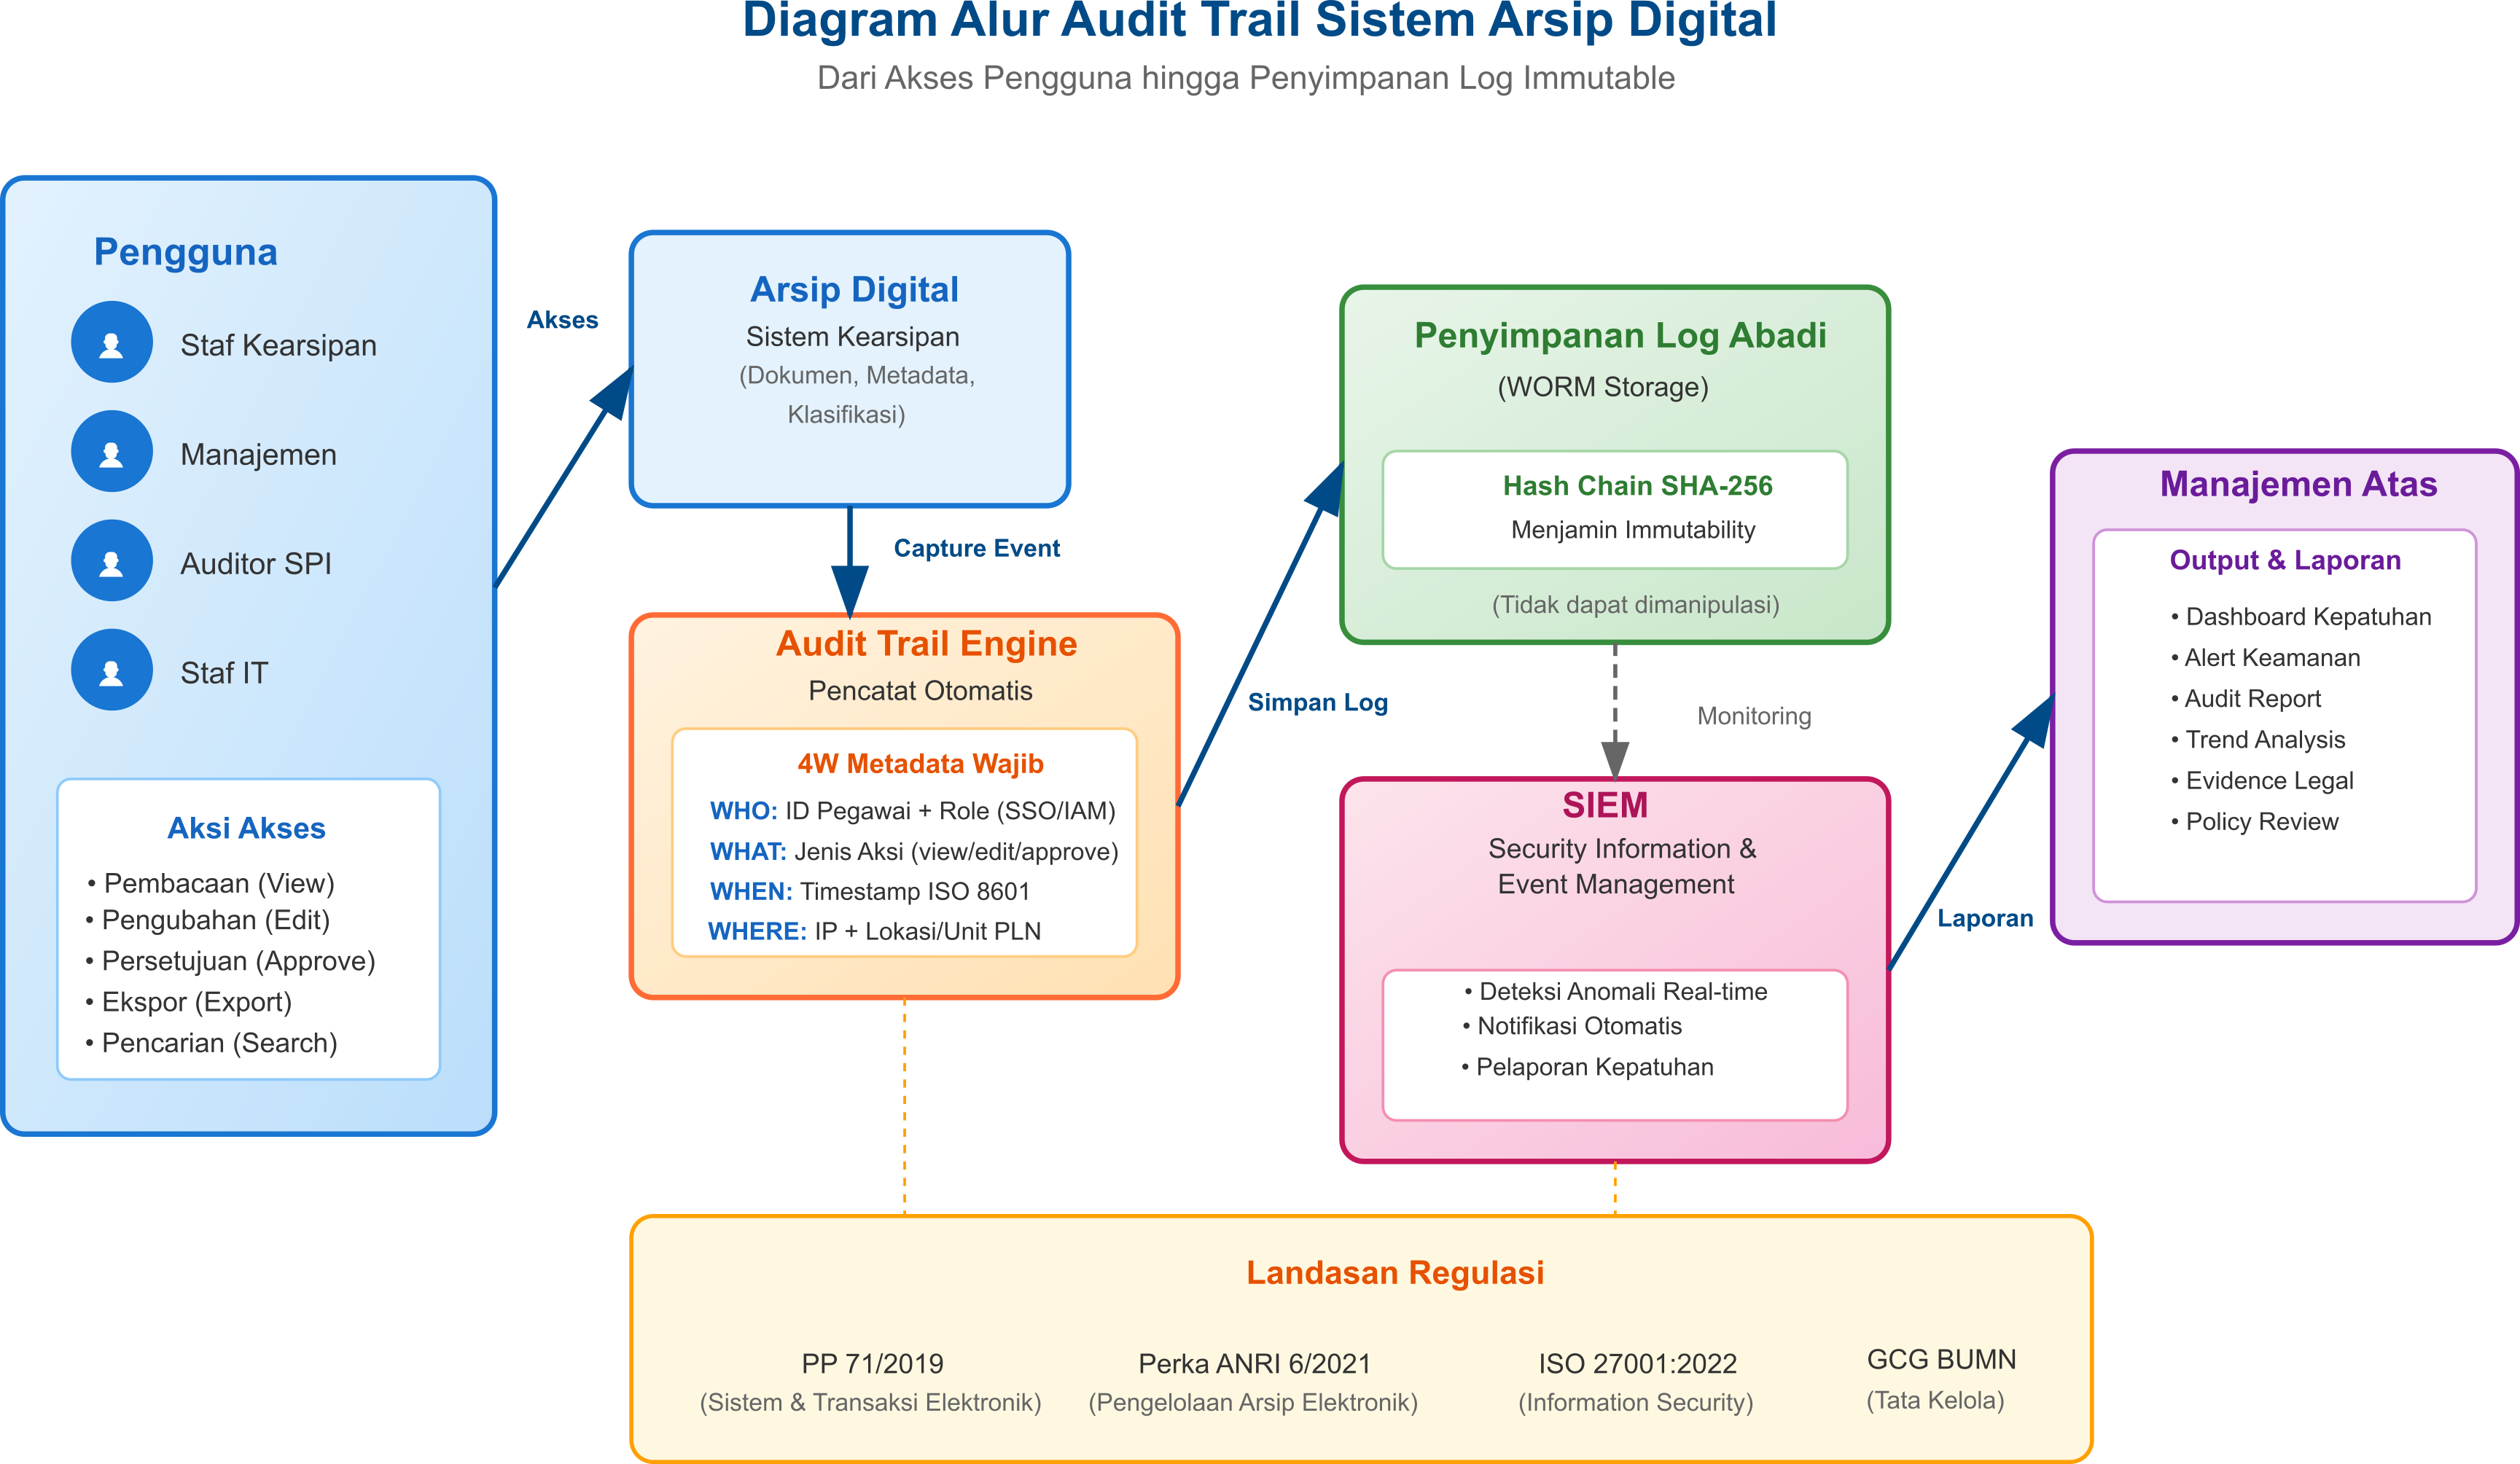
\includegraphics[width=\textwidth]{audit_v3.png}
\caption{Diagram Alur Audit Trail Sistem Arsip Digital PLN -- Dari Akses Pengguna hingga Penyimpanan Log Immutable}
\label{fig:audit-trail-flow}
\end{figure}

\small Gambar \ref{fig:audit-trail-flow} memperlihatkan alur audit trail secara menyeluruh dalam konteks kearsipan digital PLN. Pada sisi kiri, Pengguna PLN (staf kearsipan, manajemen, auditor, staf IT) mengakses Arsip Digital melalui sistem kearsipan. Setiap interaksi -- baik berupa pembacaan, pengubahan, persetujuan, maupun ekspor -- secara otomatis ditangkap oleh Audit Trail Engine yang merekam 4W metadata wajib: WHO (ID Pegawai + Role melalui SSO/IAM -- sistem manajemen identitas dan akses terpusat), WHAT (jenis aksi: akses, ubah, hapus, ekspor), WHEN (timestamp ISO 8601 presisi tinggi), dan WHERE (IP Address + Lokasi/Unit PLN). Hasil pencatatan disimpan dalam Penyimpanan Log Abadi dengan kebijakan Write-Once-Read-Many (WORM) yang dihubungkan melalui hash chain SHA-256 untuk menjamin immutability. Seluruh log secara waktu nyata dipantau oleh SIEM yang melakukan deteksi anomali, notifikasi otomatis, dan pelaporan kepatuhan kepada Manajemen Atas.

\needspace{4\baselineskip}

\section{Kerangka 4W \& Field Metadata Wajib}
Audit trail yang bermakna bagi tata kelola korporasi bukan sekadar log teknis berisi deretan kode dan timestamp, melainkan rekonstruksi digital dari setiap interaksi manusia dan sistem dengan aset informasi kritis. Kerangka 4W (Who, What, When, Where) adalah fondasi yang menjadikan log tersebut dapat dipertanggungjawabkan di hadapan regulator, auditor eksternal, dan pengadilan. Bagi Manajemen Atas, memahami 4W berarti memahami empat pertanyaan kunci yang selalu diajukan dalam investigasi insiden keamanan, temuan audit, atau sengketa hukum terkait arsip digital.

\begin{itemize}[leftmargin=*]
    \item WHO -- Identitas dan Peran: Tidak cukup mencatat nama pengguna; sistem wajib mencatat kombinasi ID Pegawai, Peran (Role), dan Unit Organisasi melalui SSO/IAM. Mengapa ini penting? Karena dalam konteks GCG dan TARIF, akuntabilitas individual adalah prasyarat. Jika log hanya mencatat ``User123'', organisasi tidak dapat membuktikan siapa yang bertanggung jawab atas suatu tindakan. WHO yang akurat juga memungkinkan Manajemen Atas untuk melakukan analisis pola akses: apakah seorang GM yang tidak biasanya mengakses arsip keuangan tiba-tiba mengunduhnya pada dini hari? Apakah akun staf kearsipan digunakan untuk mengakses kontrak pembangkit yang seharusnya di luar wewenangnya? Tanpa WHO yang terautentikasi kuat, seluruh audit trail kehilangan kekuatan hukumnya.

    \item WHAT -- Jenis Aksi: Setiap interaksi harus diklasifikasikan secara eksplisit: Create, Read, Update, Delete, Approve, Reject, Export, atau Reclassify. Bukan cukup dengan kata ``diakses''. Dalam perspektif manajemen risiko, perbedaan antara ``Read'' dan ``Export'' adalah perbedaan antara paparan internal dan potensi kebocoran eksternal. Perbedaan antara ``Update'' dan ``Reclassify'' adalah perbedaan antara perubahan konten dan perubahan status keamanan yang dapat membuka akses bagi pihak yang sebelumnya tidak berwenang. WHAT yang terstruktur memungkinkan SIEM untuk memicu aturan deteksi anomali yang spesifik, misalnya: ``Jika WHAT = Export AND CLASSIFICATION = Vital AND TIME = Outside Business Hours, maka trigger eskalasi ke VP Cyber Security.''

    \item WHEN -- Waktu Presisi Tinggi: Timestamp wajib menggunakan format ISO 8601 dengan presisi minimal milidetik dan disinkronkan melalui Network Time Protocol (NTP). Dalam investigasi insiden keamanan, urutan kronologis menentukan sebab-akibat. Jika timestamp tidak presisi atau tidak tersinkronisasi antar-sistem, Manajemen Atas tidak dapat membuktikan urutan kejadian -- misalnya, apakah ekspor arsip terjadi sebelum atau sesudah pencabutan hak akses pegawai yang resign? Dalam proses hukum, keraguan kronologis dapat melemahkan posisi organisasi.

    \item WHERE -- Sumber dan Lokasi: Pencatatan harus mencakup IP Address, nama sistem/aplikasi, dan lokasi geografis/unit organisasi. WHERE memungkinkan deteksi akses dari lokasi yang tidak biasa (misal: akun pegawai di Jakarta diakses dari luar negeri) atau dari perangkat yang tidak terdaftar. Bagi PLN dengan infrastruktur tersebar di seluruh Indonesia, WHERE juga menjadi dasar analisis risiko geografis: akses ke arsip vital dari unit di wilayah rawan bencana mungkin memerlukan kontrol tambahan.
\end{itemize}

Dalam kerangka regulasi nasional, keempat elemen 4W ini bukan pilihan melainkan kewajiban. PP 71/2019 mensyaratkan bahwa setiap sistem elektronik yang menyimpan data penting wajib memiliki audit trail yang ``lengkap, akurat, dan dapat dipertanggungjawabkan''\footnote{PP 71/2019, Penyelenggaraan Sistem dan Transaksi Elektronik, LNRI 196 (2019).}. Perka ANRI 6/2021 lebih spesifik lagi dengan menetapkan bahwa arsip elektronik wajib memiliki metadata yang mencakup identitas pembuat, waktu pembentukan, dan jejak pengelolaan\footnote{Perka ANRI 6/2021, Pengelolaan Arsip Elektronik, BNRI 541 (2021).}. Ketika digabungkan, 4W memenuhi kedua regulasi tersebut dan memberikan landasan bagi \textit{non-repudiation} -- bukti bahwa seseorang tidak dapat menyangkal telah melakukan suatu tindakan.

Untuk memastikan implementasi 4W tidak hanya bersifat deklaratif, Modul ini mewajibkan penerapan 14 Field Metadata Audit pada setiap entri log. Tabel berikut memperinci field tersebut, bersama dengan sumber data dan status kepatuhannya:

\begingroup
\small
\begin{xltabular}{\textwidth}{@{} c >{\raggedright\arraybackslash}X >{\raggedright\arraybackslash}X c @{}}
\caption{14 Field Metadata Audit Trail (12 Wajib + 2 Semi-Mandatory)}\\
\toprule
\textbf{Kode} & \textbf{Nama Field} & \textbf{Sumber Data} & \textbf{Status} \\
\midrule
\endfirsthead

\multicolumn{4}{@{}l}{\small\textit{Lanjutan Tabel \thetable}}\\
\toprule
\textbf{Kode} & \textbf{Nama Field} & \textbf{Sumber Data} & \textbf{Status} \\
\midrule
\endhead

\bottomrule
\endfoot

DOC\_ID & ID Dokumen Unik & Sistem Nomor & Wajib \\
TIMESTAMP & Waktu Aksi (ISO 8601) & System Clock & Wajib \\
HASH\_SHA256 & Nilai Hash Integritas & Cryptographic Module & Wajib \\
CREATOR\_ROLE & Peran Pengguna & IAM/SSO & Wajib \\
AUDIT\_LOG\_ID & ID Log Immutable & SIEM/Audit Engine & Wajib \\
CLASSIFICATION & Tingkat Keamanan & Policy Engine & Wajib \\
RETENTION\_RULE & Aturan Retensi & Schedule DB & Wajib \\
ASSET\_ID & Referensi Aset PLN & SAP-PM/AMS & Wajib \\
CONTRACT\_REF & Referensi Kontrak & E-Proc/Legal & Wajib \\
LOCATION\_GIS & Lokasi Operasional & Master Data & Wajib \\
INTEGRITY\_HASH & Verifikasi Perubahan & Hash Module & Wajib \\
AUDIT\_TRAIL\_REF & Log Terkait & Chain Log & Wajib \\
CONTENT\_DESC & Ringkasan Isi & NLP/Input & Semi \\
SEARCH\_TAGS & Kata Kunci Terkontrol & Thesaurus & Semi \\
\end{xltabular}
\endgroup

\noindent Membaca Tabel untuk Keputusan Manajemen: Dua belas field bertanda \textit{Wajib} membentuk \textit{minimum viable audit log} yang harus ada agar entri log memiliki kekuatan hukum dan dapat digunakan sebagai bukti investigasi. Tanpa salah satu dari 12 field ini, log tersebut berisiko ditolak oleh auditor eksternal atau regulator karena dianggap tidak lengkap. Misalnya, jika HASH\_SHA256 tidak tercatat, organisasi tidak dapat membuktikan bahwa log tersebut tidak dimanipulasi. Jika CONTRACT\_REF tidak tercatat, Manajemen Atas tidak dapat melakukan korelasi antara aktivitas arsip dengan kontrak pembangkit tertentu yang sedang diaudit BPK.

Dua field \textit{Semi-Mandatory} (CONTENT\_DESC dan SEARCH\_TAGS) bersifat pendukung analisis, bukan prasyarat hukum. CONTENT\_DESC memungkinkan Manajemen Atas untuk memahami konteks aktivitas tanpa harus membuka dokumen asli, sedangkan SEARCH\_TAGS memfasilitasi pencarian cepat saat investigasi. Kedua field ini sangat disarankan untuk arsip Vital dan Rahasia, meskipun tidak diwajibkan secara regulasi.

\begin{plnbox}[Risiko Jika Metadata Audit Tidak Lengkap]
Ketidaklengkapan metadata audit bukan sekadar temuan teknis -- melainkan temuan tata kelola yang dapat berakibat fatal. Jika terjadi kebocoran arsip kontrak pembangkit dan log audit tidak mencatat WHO dengan ID SSO yang jelas, organisasi tidak dapat menunjukkan siapa yang bertanggung jawab. Jika WHAT tidak mencatat jenis aksi ``Export'', organisasi tidak dapat membuktikan bahwa data benar-benar telah keluar dari sistem. Jika WHEN tidak presisi, pihak hukum dapat mengajukan keraguan kronologis. Dan jika WHERE tidak tercatat, organisasi kehilangan kemampuan untuk mendeteksi akses dari lokasi tidak sah. Singkatnya: metadata yang tidak lengkap mengubah audit trail dari ``bukti tak terbantahkan'' menjadi ``kumpulan data yang dapat dipersoalkan''.
\end{plnbox}

\needspace{4\baselineskip}

\section{Kategori Event Audit Level Bisnis}
Bagi Manajemen Atas, memahami \textit{apa} yang harus dicatat dalam audit trail jauh lebih strategis daripada memahami \textit{bagaimana} sistem mencatatnya secara teknis. Kategori event adalah lensa bisnis yang mengubah ribuan baris log mentah menjadi informasi intelijen risiko. Setiap kategori merepresentasikan vektor ancaman atau titik akuntabilitas yang berbeda. Jika salah satu kategori tidak tercakup, organisasi memiliki \textit{blind spot} -- area di mana aktivitas berisiko tinggi dapat terjadi tanpa terdeteksi.

Pemilihan kategori event harus didasarkan pada pertanyaan: ``Aktivitas apa yang, jika tidak tercatat, akan membuat organisasi tidak mampu menjawab pertanyaan regulator atau menemukan pelaku kebocoran data?'' Berikut adalah lima kategori event yang wajib tercakup dalam mekanisme audit trail arsip digital PLN, dengan penjelasan strategis dan skenario nyata untuk masing-masing:

\begingroup
\small
\setlength{\tabcolsep}{4pt}
\renewcommand{\arraystretch}{1.2}
\begin{longtable}{@{}>{\raggedright\arraybackslash}p{2.2cm} >{\raggedright\arraybackslash}p{2.8cm} p{8.7cm}@{}}
\caption{Kategori Event Audit Trail untuk Arsip Digital -- Perspektif Tata Kelola}
\label{tab:kategori-event-audit}\\
\toprule
\textbf{Kategori} & \textbf{Jenis Event} & \textbf{Relevansi Bisnis / Skenario PLN} \\
\midrule
\endfirsthead

\multicolumn{3}{@{}l}{\small\textit{Lanjutan Tabel \thetable}}\\
\toprule
\textbf{Kategori} & \textbf{Jenis Event} & \textbf{Relevansi Bisnis / Skenario PLN} \\
\midrule
\endhead

\bottomrule
\endfoot

Akses & Login, logout, view, search & Deteksi rekognisi ancaman: Memantau siapa yang ``melihat'' arsip sensitif dan kapan. \textit{Skenario:} Akun staf administrasi unit pembangkitan secara berulang melakukan \textit{search} dan \textit{view} terhadap arsip kontrak Pemeliharaan Infrastruktur Transmisi di luar jam kerja. Tanpa log kategori Akses, pola ini tidak terdeteksi hingga terjadi kebocoran. \\
\addlinespace
Perubahan & Create, update, rename, reclassify & Integritas data dan jejak modifikasi: Melacak setiap perubahan konten dan metadata arsip. \textit{Skenario:} Nilai kontrak pembangkit listrik diubah dalam sistem e-Procurement setelah proses tender selesai. Tanpa log \textit{update} dengan field WHAT dan WHO yang jelas, Manajemen Atas tidak dapat membedakan antara perubahan resmi dan manipulasi data. Perubahan \textit{reclassify} sangat kritis karena dapat menurunkan tingkat keamanan arsip secara diam-diam. \\
\addlinespace
Persetujuan & Approve, reject, revoke & Akuntabilitas keputusan kritis: Menjamin bahwa setiap keputusan yang mengikat secara hukum dapat dipertanggungjawabkan kepada individu spesifik. \textit{Skenario:} Penyetujuan pengalihan dokumen RUPS kepada pihak ketiga. Jika log persetujuan tidak ada atau tidak terikat dengan TTE (Tanda Tangan Elektronik Tersertifikasi), keputusan tersebut dapat dibatalkan atau disangkal di pengadilan, membahayakan posisi hukum PLN. \\
\addlinespace
Ekspor & Download, print, share, export & Pengendalian risiko kebocoran: Kategori paling kritis dari perspektif kebocoran data. \textit{Skenario:} Seorang manajer mengunduh 500 dokumen arsip Rahasia ke laptop pribadi sehari sebelum mengajukan pengunduran diri. Tanpa log \textit{download} yang terkorelasi dengan event WHO dan WHERE, Manajemen Atas baru mengetahui kebocoran setelah data muncul di media atau pesaing. Setiap event ekspor harus memicu review otomatis jika volume atau frekuensinya di luar pola normal. \\
\addlinespace
Sistem & Backup, restore, delete, archive & Jaminan ketersediaan dan integritas: Mencatat operasi yang memengaruhi keberadaan arsip itu sendiri. \textit{Skenario:} Seorang administrator sistem secara tidak sengaja (atau disengaja) menghapus arsip Vital dalam jumlah besar tanpa otorisasi. Tanpa log \textit{delete} dengan integritas hash, organisasi tidak dapat membuktikan bahwa penghapusan itu terjadi, siapa pelakunya, dan kapan waktunya -- informasi yang krusial untuk proses pemulihan data dan disiplin pegawai. Log \textit{restore} juga penting untuk memastikan data yang dipulihkan adalah versi yang benar dan tidak terkontaminasi. \\
\end{longtable}
\endgroup

\noindent Mengapa Kelima Kategori Ini Tidak Boleh Dikurangi? Setiap kategori memenuhi kebutuhan intelijen risiko yang berbeda. Kategori \textit{Akses} dan \textit{Ekspor} menjawab pertanyaan \textit{siapa yang memiliki niat jahat atau perilaku tidak wajar}. Kategori \textit{Perubahan} dan \textit{Persetujuan} menjawab pertanyaan \textit{siapa yang mengubah fakta dan siapa yang bertanggung jawab atas keputusan}. Kategori \textit{Sistem} menjawab pertanyaan \textit{apakah arsip itu masih ada dan utuh}. Kelima kategori ini bersinergi: investigasi kebocoran arsip Vital biasanya memerlukan korelasi lintas-kategori -- misalnya, seorang pegawai melakukan \textit{view} berulang (Akses), kemudian melakukan \textit{export} massal (Ekspor), dan beberapa jam kemudian mengajukan resign. Tanpa kelima kategori tercatat secara konsisten, Manajemen Atas kehilangan kemampuan untuk mengkonstruksi narasi insiden secara utuh.

\begin{plnbox}[Panduan Review Berkala untuk Manajemen Atas]
Manajemen Atas tidak perlu membaca log mentah, tetapi perlu memastikan tim keamanan informasi menyajikan \textit{dashboard kategori event} secara rutin dengan indikator berikut: (1) Tren Akses Rahasia/Vital di luar jam kerja -- peningkatan tren dapat menandakan ancaman internal; (2) Volume Ekspor per pegawai per bulan -- outlier menandakan potensi eksfiltrasi data; (3) Jumlah Persetujuan tanpa TTE -- indikasi kelemahan kontrol kekuatan hukum; (4) Event Sistem (delete/restore) tanpa tiket perubahan -- indikasi aktivitas administrator yang tidak terkendali; dan (5) Perubahan Reclassify -- setiap perubahan klasifikasi ke bawah wajib ditinjau manual karena berpotensi membuka akses yang sebelumnya tertutup.
\end{plnbox}

\needspace{4\baselineskip}

\section{Langkah-Langkah Perancangan Mekanisme Audit Trail}
Perancangan audit trail tingkat tata kelola bagi Manajemen Atas berfokus pada apa yang harus dicatat, bagaimana memantau kepatuhannya, dan bagaimana menindaklanjuti anomali -- bukan pada detail implementasi teknis.

\begin{enumerate}[leftmargin=*]
    \item Tentukan Cakupan dan Retensi. Manajemen Atas menetapkan arsip apa saja yang wajib memiliki audit trail -- minimal arsip Rahasia dan Vital. Tentukan juga berapa lama log harus disimpan: minimal sesuai masa retensi arsip terkait. Misalnya, jika arsip vital disimpan 25 tahun, log auditnya juga harus disimpan selama itu.
    \item Validasi Kelengkapan Metadata. Pastikan tim IT mengimplementasikan 14 field metadata (Tabel 2) untuk setiap event. Manajemen Atas tidak perlu memahami implementasi teknisnya, tetapi harus meminta bukti bahwa seluruh field tercatat -- misalnya melalui contoh laporan log yang dihasilkan sistem.
    \item Tetapkan Mekanisme Pemantauan. Manajemen Atas menunjuk tim yang bertanggung jawab memantau laporan audit trail secara berkala (misal: mingguan untuk arsip vital, bulanan untuk arsip rahasia) dan menetapkan format laporan yang diterima.
    \item Tetapkan Mekanisme Eskalasi. Jika terdeteksi anomali -- misalnya arsip Rahasia diunduh di luar jam kerja oleh peran yang tidak biasanya mengakses -- siapa yang dihubungi dalam 1 jam, 4 jam, 24 jam? Manajemen Atas menyetujui prosedur eskalasi ini.
    \item Pastikan Kepatuhan Regulasi. Audit trail harus memenuhi PP 71/2019 dan Perka ANRI 6/2021. Manajemen Atas meminta tim untuk memverifikasi kepatuhan dan menunjukkan bukti saat audit eksternal.
\end{enumerate}

Pertanyaan kunci untuk Manajemen Atas: ``Jika hari ini terjadi kebocoran arsip vital, apakah kita bisa menunjukkan siapa yang mengakses, mengubah, atau mengekspor arsip tersebut dalam 6 bulan terakhir -- lengkap dengan waktu, peran, dan alasan aksesnya?''

\begin{plnbox}[Ringkasan untuk Manajemen Atas -- Bab 2]
Audit trail mewujudkan keterlacakan (traceability) -- yaitu kemampuan untuk merekonstruksi secara lengkap siapa yang mengakses, mengubah, atau mengekspor arsip tertentu pada waktu tertentu. Tiga pesan kunci dari bab ini: (1) audit trail bukan log teknis semata, melainkan bukti hukum yang sah di mata regulator (PP 71/2019, Perka ANRI 6/2021); (2) kekekalan log (immutability) melalui hash chain menjamin bahwa tidak ada pihak -- termasuk admin sistem -- yang dapat memanipulasi catatan tanpa terdeteksi; dan (3) deteksi anomali secara waktu nyata oleh SIEM lebih bernilai daripada investigasi pascakejadian setelah kerusakan sudah terjadi.
\end{plnbox}

\needspace{4\baselineskip}

\section{Aktivitas Workshop (30 Menit)}
\begin{enumerate}[leftmargin=*]
    \item Gambar alur audit trail dari penciptaan $\rightarrow$ validasi $\rightarrow$ penyimpanan.
    \item Lengkapi template 14 field untuk 1 jenis arsip kritis unit Anda.
    \item Tentukan mekanisme eskalasi jika hash integrity gagal verifikasi.
\end{enumerate}

\begin{outputbox}
\textbf{Portofolio 2 (Pilar 2: Audit Trail):} Diagram Alur Audit Trail + Template Log 14 Field. Dinilai berdasarkan kemampuan peserta merancang mekanisme audit trail otomatis yang merekam setiap akses dan perubahan arsip, kelengkapan 4W, kejelasan immutability, dan kesesuaian dengan regulasi PP 71/2019.
\end{outputbox}

% ============================================================
\chapter{Kebijakan Keamanan Terintegrasi dengan ISMS}
(Kriteria Penilaian 4.4.3 -- Target Kompetensi 3)
% ============================================================

Mengapa bab ini berurutan setelah Audit Trail? RBAC (Pilar 1) mengontrol akses dan Audit Trail (Pilar 2) mencatat akses. Namun, kedua mekanisme tersebut memerlukan payung hukum dan kerangka tata kelola agar memiliki kekuatan mengikat di level organisasi. Tanpa kebijakan keamanan yang disahkan oleh Manajemen Atas, RBAC dan audit trail hanyalah konfigurasi teknis yang tidak memiliki dasar hukum -- dan dapat dengan mudah diabaikan atau diubah tanpa pertanggungjawaban. Kebijakan keamanan (Pilar 3) memberikan landasan legitimasi bagi seluruh kontrol keamanan, sekaligus memastikan keselarasan dengan standar internasional (ISO 27001), regulasi nasional (PP 71/2019), dan prinsip GCG BUMN (TARIF).

Bab ini mendukung pencapaian Pilar 3: Kebijakan Keamanan -- peserta mampu merumuskan kebijakan keamanan yang terintegrasi dengan sistem manajemen keamanan informasi organisasi. Kebijakan keamanan arsip tidak boleh berdiri sendiri. Ia harus menjadi bagian tak terpisahkan dari Sistem Manajemen Keamanan Informasi (ISMS) organisasi dan mendukung prinsip GCG BUMN (TARIF).

Dua kerangka standar internasional menjadi rujukan utama dalam bab ini. Pertama, ISO/IEC 27001:2022 yang diterbitkan oleh International Organization for Standardization (ISO) merupakan kerangka manajemen keamanan informasi yang paling banyak diadopsi secara global, mencakup siklus PDCA dan 93 kontrol keamanan. Kedua, standar dan panduan yang diterbitkan oleh NIST (National Institute of Standards and Technology) -- sebuah lembaga riset dan standar di bawah Departemen Perdagangan Amerika Serikat yang menghasilkan kerangka keamanan siber praktikal seperti Cybersecurity Framework, SP 800-53 (kontrol keamanan), dan SP 800-207 (\textit{Zero Trust Architecture}). Panduan NIST bersifat tidak wajib tetapi secara luas diakui sebagai referensi terbaik dalam perancangan kebijakan keamanan informasi.

\needspace{4\baselineskip}

\section{Integrasi dengan ISO/IEC 27001:2022}

ISO/IEC 27001:2022 mewajibkan organisasi menerapkan siklus perbaikan berkelanjutan yang dikenal sebagai PDCA (Plan-Do-Check-Act). Siklus ini memastikan bahwa kebijakan keamanan arsip bukan sekadar dokumen statis, melainkan kerangka kerja yang terus berevolusi mengikuti perubahan ancaman, regulasi, dan kebutuhan organisasi. Gambar \ref{fig:pdca-cycle} menunjukkan penerapan siklus PDCA dalam konteks keamanan arsip digital PLN.

%% ============================================================
%% GAMBAR 3.1 — Siklus PDCA
%% Unduh: https://upload.wikimedia.org/wikipedia/commons/7/7a/PDCA_Cycle.svg
%% Simpan sebagai: gambar/PDCA_Cycle.svg
%% ============================================================

\begin{figure}[H]
\centering
\resizebox{0.50\textwidth}{!}{%
\begin{tikzpicture}[
  box/.style={draw=#1, fill=#1!10, rounded corners=4pt,
    line width=0.8pt, minimum width=2.4cm, minimum height=1.2cm,
    font=\small, align=center},
  arr/.style={-{Stealth[length=5pt]}, line width=1pt, #1}
]
\node[box=plnblue]   (plan)  at (-2, 1.5) {\textbf{\color{plnblue}PLAN}\\[-1pt]
  {\scriptsize Kebijakan \& Risiko}};
\node[box=green!50!black] (do)    at ( 2, 1.5) {\textbf{\color{green!50!black}DO}\\[-1pt]
  {\scriptsize Implementasi Kontrol}};
\node[box=orange!80!black] (check) at ( 2,-1.5) {\textbf{\color{orange!80!black}CHECK}\\[-1pt]
  {\scriptsize Audit \& Evaluasi}};
\node[box=red!70!black]   (act)   at (-2,-1.5) {\textbf{\color{red!70!black}ACT}\\[-1pt]
  {\scriptsize Perbaikan Berkelanjutan}};
\node[font=\scriptsize\bfseries, text=gray] at (0,0) {ISO 27001:2022};
% Curved arrows
\draw[arr=plnblue]       (plan.east)  -- (do.west);
\draw[arr=green!50!black]  (do.south)    -- (check.north);
\draw[arr=orange!80!black] (check.west)  -- (act.east);
\draw[arr=red!70!black]    (act.north)   -- (plan.south);
\end{tikzpicture}%
}
\caption{Siklus PDCA (Plan-Do-Check-Act) -- Fondasi ISO/IEC 27001:2022\\
\small Sumber: Wikimedia Commons -- PDCA Cycle
(\url{https://commons.wikimedia.org/wiki/File:PDCA_Cycle.svg})}
\label{fig:pdca-cycle}
\end{figure}

\small Gambar \ref{fig:pdca-cycle} menunjukkan siklus PDCA yang merupakan fondasi dari seluruh kerangka ISO/IEC 27001:2022. Dalam konteks keamanan arsip digital PLN, siklus ini diterjemahkan menjadi: (1) Plan -- merancang kebijakan keamanan arsip, mengidentifikasi risiko, dan menetapkan kontrol; (2) Do -- mengimplementasikan kontrol RBAC, backup, dan pemantauan; (3) Check -- melakukan audit internal dan evaluasi kepatuhan; serta (4) Act -- melakukan perbaikan berkelanjutan berdasarkan temuan audit dan insiden keamanan.

Arsip digital dikategorikan sebagai Aset Informasi Kritis. Dalam kerangka ISO/IEC 27001:2022 (edisi ke-3)\footnote{ISO/IEC 27001:2022, Annex A (93 kontrol: A.5 organisasi, A.6 SDM, A.7 fisik, A.8 teknologi).}, keamanan arsip digital menyentuh beberapa kelompok kontrol utama yang saling melengkapi. Integrasi dilakukan melalui:
\begin{itemize}[leftmargin=*]
    \item A.5.9--A.5.14 (Asset Management): Inventarisasi, klasifikasi, dan penentuan owner arsip -- memastikan setiap arsip memiliki penanggung jawab yang jelas.
    \item A.5.1--A.5.2 (Information Security Policies): Penyelarasan kebijakan induk kearsipan dengan kebijakan keamanan informasi korporasi.
    \item A.8.8--A.8.17 (Operations Security): Prosedur operasional backup, monitoring log, dan penanganan insiden kebocoran.
\end{itemize}

%% ============================================================
%% GAMBAR 3.2 — Area Kontrol ISO/IEC 27001:2022 (Custom Diagram)
%% Desain mandiri berdasarkan standar ISO/IEC 27001:2022
%% ============================================================

Implementasi ISO/IEC 27001:2022 di organisasi sebesar PLN tidak berarti menjalankan seluruh 93 kontrol secara bersamaan dengan prioritas yang sama. Sebagian kontrol memiliki dampak langsung terhadap keamanan arsip digital — misalnya: manajemen aset, kontrol akses, kriptografi, dan kelangsungan bisnis — sementara kontrol lain bersifat pendukung (kesadaran keamanan, keamanan fisik, pengembangan sistem). Tanpa pemetaan prioritas, Manajemen Atas berisiko mengalokasikan sumber daya pada kontrol dengan dampak rendah bagi kearsipan sementara kontrol kritis terabaikan. Gambar \ref{fig:iso27001-controls} berfungsi sebagai peta jalan prioritisasi: ia menampilkan seluruh lanskap 93 kontrol dalam 4 kelompok besar sekaligus menyorot (dengan tanda {\color{orange!80!black}$\star$}) sub-kategori yang memiliki relevansi tinggi terhadap keamanan arsip digital PLN. Dengan peta ini, Manajemen Atas dapat mengambil keputusan strategis berbasis bukti: fokus investasi pada kontrol bertanda bintang terlebih dahulu, baru melengkapi kontrol pendukung sesuai ketersediaan anggaran.

\begin{figure}[H]
\centering
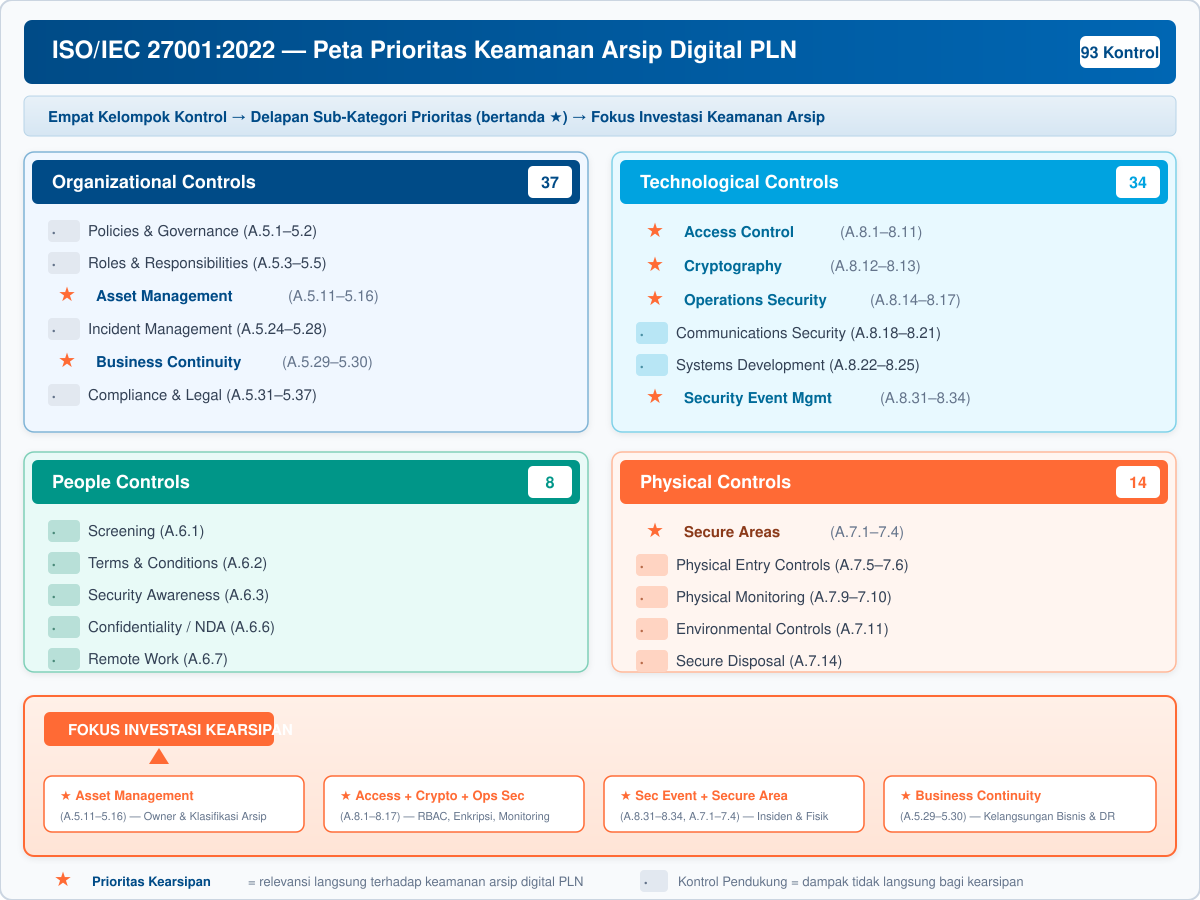
\includegraphics[width=0.75\textwidth]{iso_preview.png}
\caption{Peta Area Kontrol ISO/IEC 27001:2022 -- 93 Kontrol dalam 4 Kelompok dengan Indikator Relevansi Kearsipan\\
\small Sumber: ISO/IEC 27001:2022, diadaptasi untuk konteks PLN.}
\label{fig:iso27001-controls}
\end{figure}

Gambar \ref{fig:iso27001-controls} menyorot sub-kategori bertanda {\color{orange!80!black}$\star$} yang menjadi prioritas investasi keamanan arsip: Manajemen Aset, Business Continuity, Kontrol Akses, Kriptografi, Operasional Keamanan, dan Manajemen Insiden. Sub-kategori tanpa tanda bintang adalah kontrol pendukung yang tetap penting, namun tidak memiliki dampak langsung terhadap kearsipan. Peta ini memberikan dasar obyektif bagi Manajemen Atas untuk mengalokasikan anggaran secara proporsional.

\needspace{4\baselineskip}

\section{Tiga Prinsip Fundamental Kebijakan}

Kebijakan keamanan arsip digital dibangun di atas tiga prinsip fundamental yang bukan konsep teknis, melainkan keputusan strategis yang harus diinternalisasi oleh Manajemen Atas sebagai basis pengambilan keputusan tata kelola keamanan informasi.

\begin{enumerate}[leftmargin=*]
    \item \textit{Least Privilege:} Hak akses minimum yang diperlukan untuk menyelesaikan tugas -- lihat penjelasan detail dan skenario kearsipan PLN pada Bab~1.
    \item \textit{Defense in Depth:} Lapisan pengamanan berlapis (fisik, jaringan, aplikasi, data, kebijakan).
    \item \textit{Zero Trust:} Tidak ada akses default. Setiap permintaan diverifikasi secara eksplisit berdasarkan konteks (role, device, lokasi, waktu).
\end{enumerate}

%% ============================================================
%% GAMBAR 3.3 — Defense in Depth (Custom 5-Layer Diagram)
%% Desain mandiri dengan 5 lapisan sesuai narasi
%% ============================================================

\begin{figure}[H]
\centering
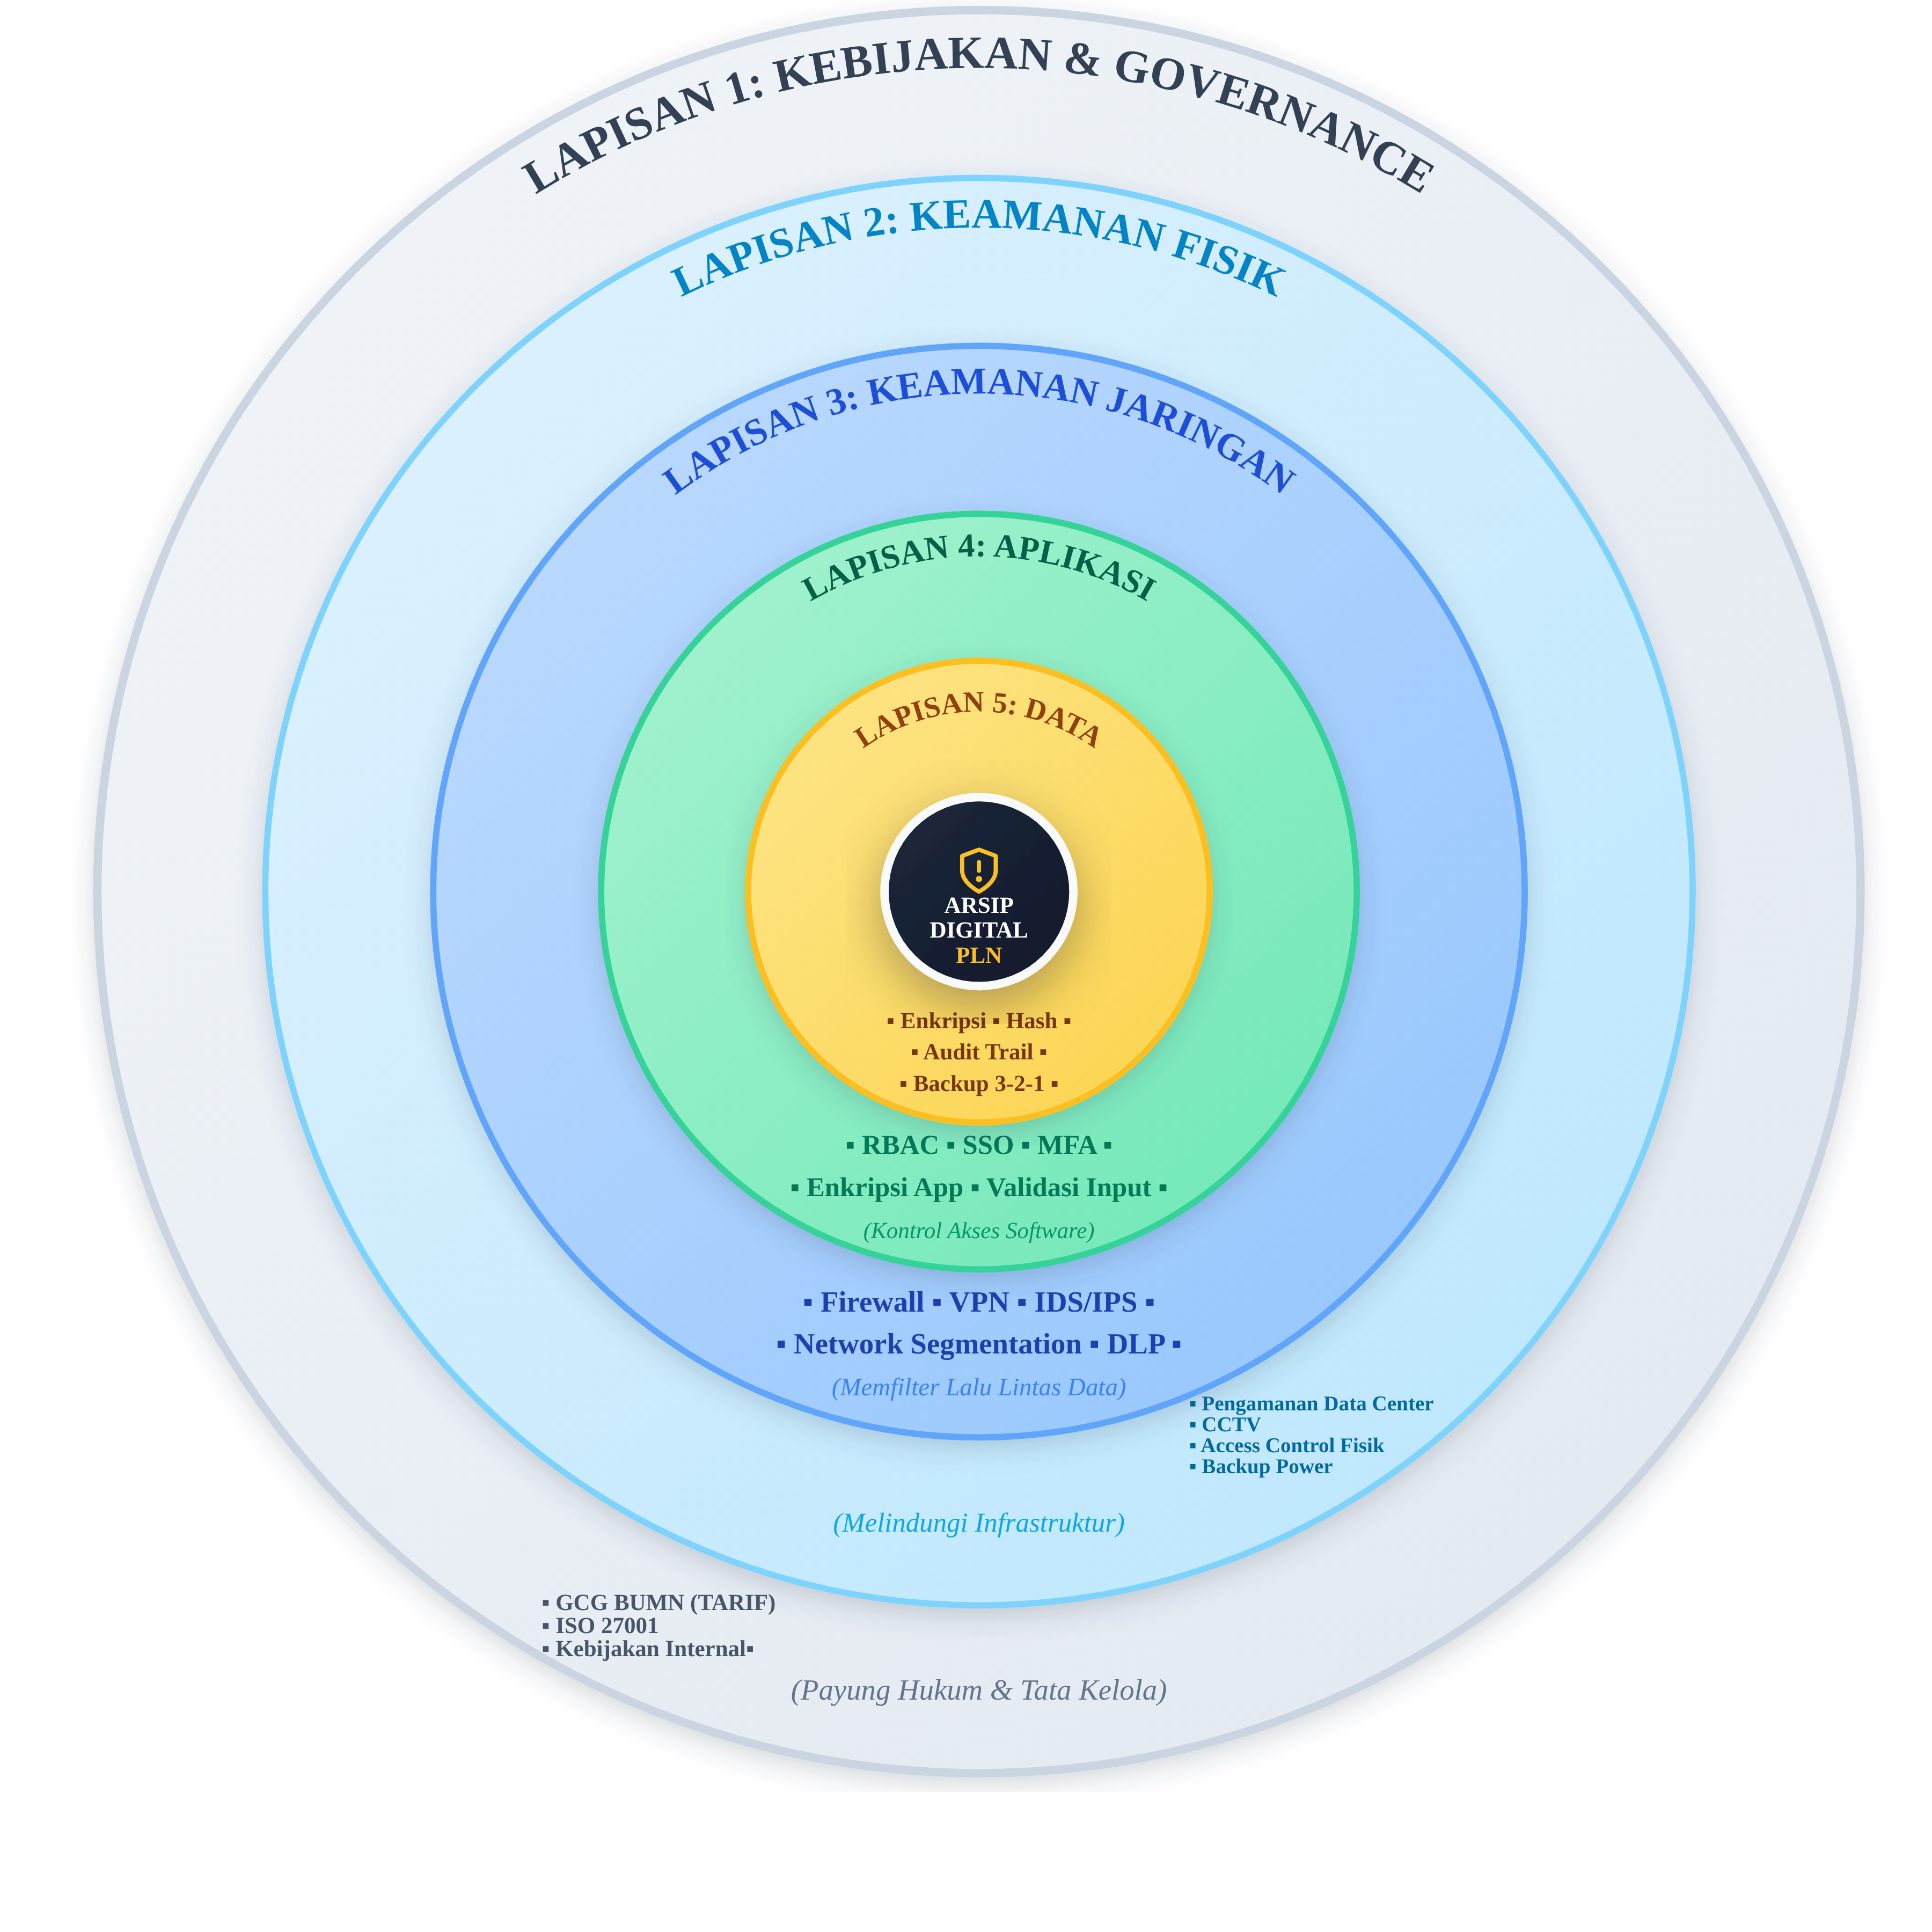
\includegraphics[width=0.60\textwidth]{defense_in_depth.png}
\caption{\textit{Defense in Depth} -- 5 Lapisan Keamanan Berlapis untuk Melindungi Arsip Digital PLN\\
\small Sumber: NIST SP 800-53.}
\label{fig:defense-in-depth}
\end{figure}

\small Gambar \ref{fig:defense-in-depth} mengilustrasikan konsep \textit{Defense in Depth} dalam konteks keamanan arsip digital PLN, yang terdiri dari 5 lapisan keamanan berlapis dari luar ke dalam. Lapisan 1 -- Kebijakan \& Governance (terluar) membentuk payung hukum dan tata kelola: GCG BUMN (TARIF), ISO 27001, dan kebijakan keamanan arsip internal PLN. Lapisan 2 -- Keamanan Fisik melindungi infrastruktur: pengamanan data center, CCTV, access control fisik, dan backup power. Lapisan 3 -- Keamanan Jaringan memfilter lalu lintas data: firewall, VPN, IDS/IPS, network segmentation, dan DLP. Lapisan 4 -- Keamanan Aplikasi mengontrol akses pada level perangkat lunak: RBAC, SSO, MFA, enkripsi aplikasi, dan validasi input. Lapisan 5 -- Keamanan Data (terdalam) melindungi inti aset: enkripsi data, hash integrity, audit trail immutable, dan backup 3-2-1. Di inti paling dalam terdapat Arsip Digital PLN sebagai aset yang dilindungi. Prinsip utamanya: tidak ada satu lapisan pun yang cukup untuk melindungi arsip secara mandiri -- jika satu lapisan berhasil ditembus, lapisan berikutnya masih memberikan proteksi.

%% ============================================================
%% GAMBAR 3.4 — Zero Trust Architecture (NIST SP 800-207)
%% Sumber: NIST SP 1800-35 — General ZTA Reference Architecture (Figure 1)
%% Unduh: https://pages.nist.gov/zero-trust-architecture/_images/Architecture-Figure1.png
%% Simpan sebagai: gambar/NIST_Zero_Trust_Architecture.png
%% ============================================================

\begin{figure}[H]
\centering
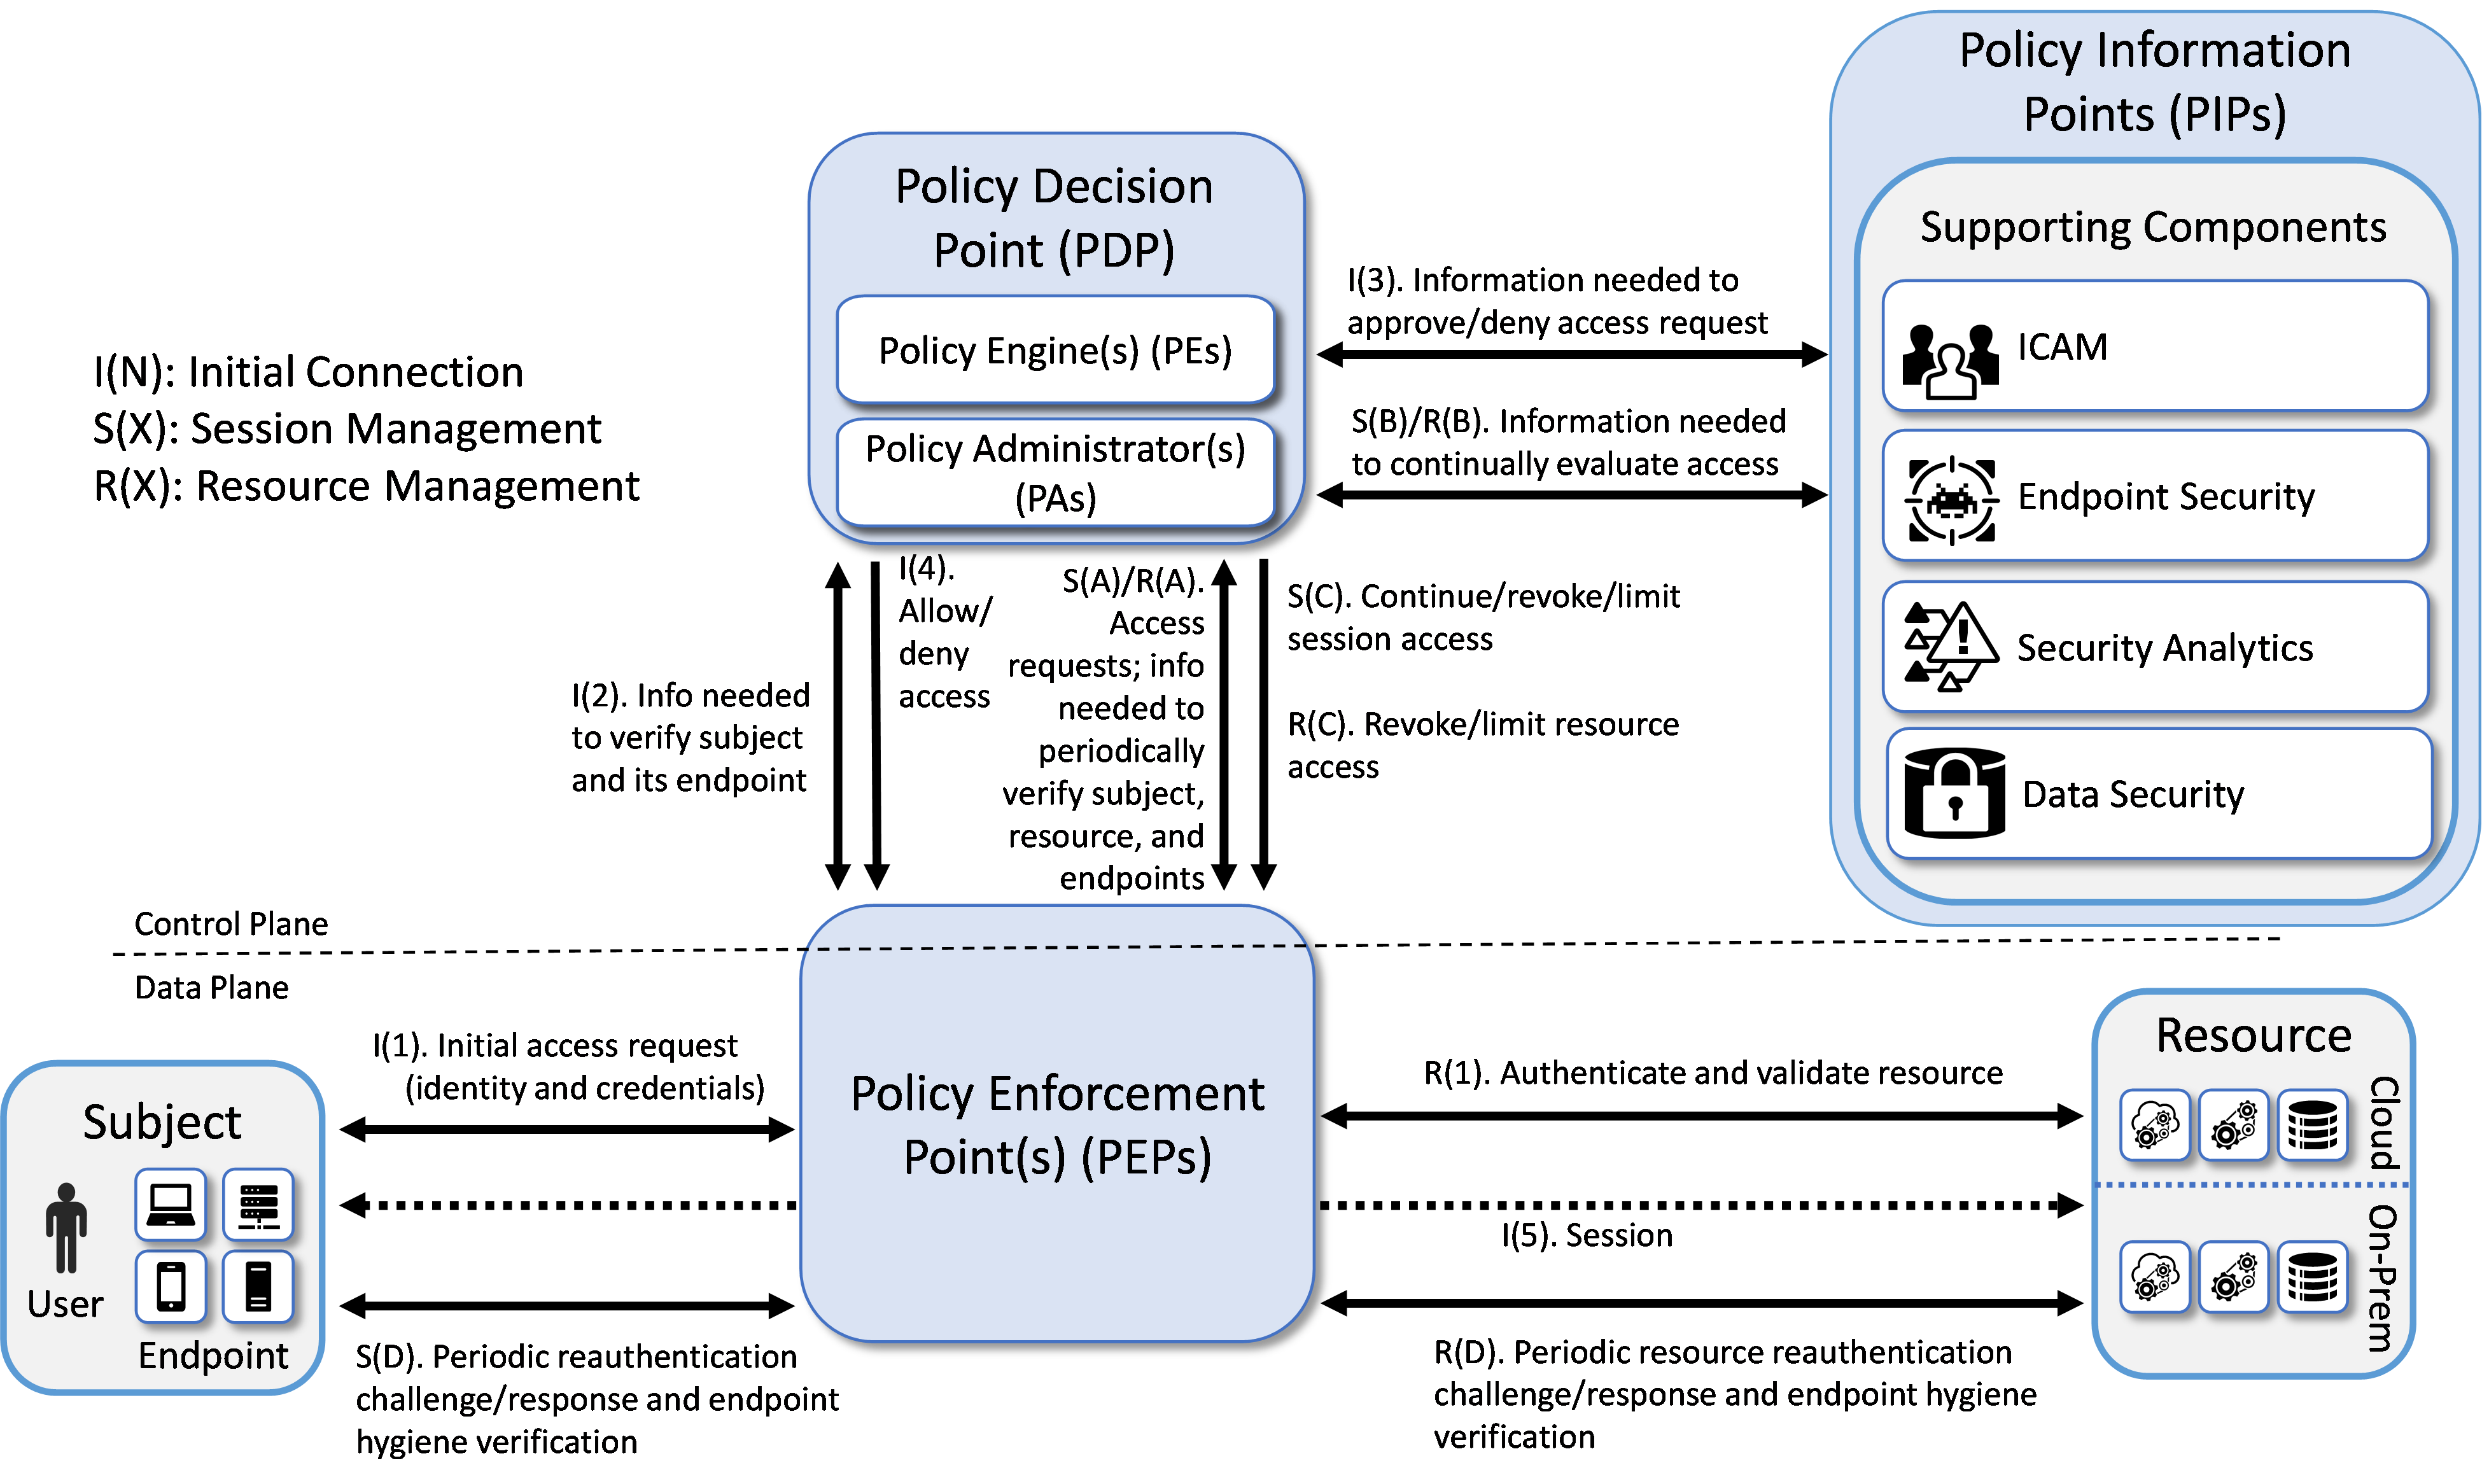
\includegraphics[width=0.85\textwidth,height=0.35\textheight,keepaspectratio]{gambar/NIST_Zero_Trust_Architecture.png}
\caption{Arsitektur \textit{Zero Trust} Referensi NIST\\
\small Sumber: NIST SP 1800-35, Figure 1 (Public Domain).}
\label{fig:zero-trust}

\vspace{1em}
\rule{0.6\textwidth}{0.4pt}
\vspace{1em}

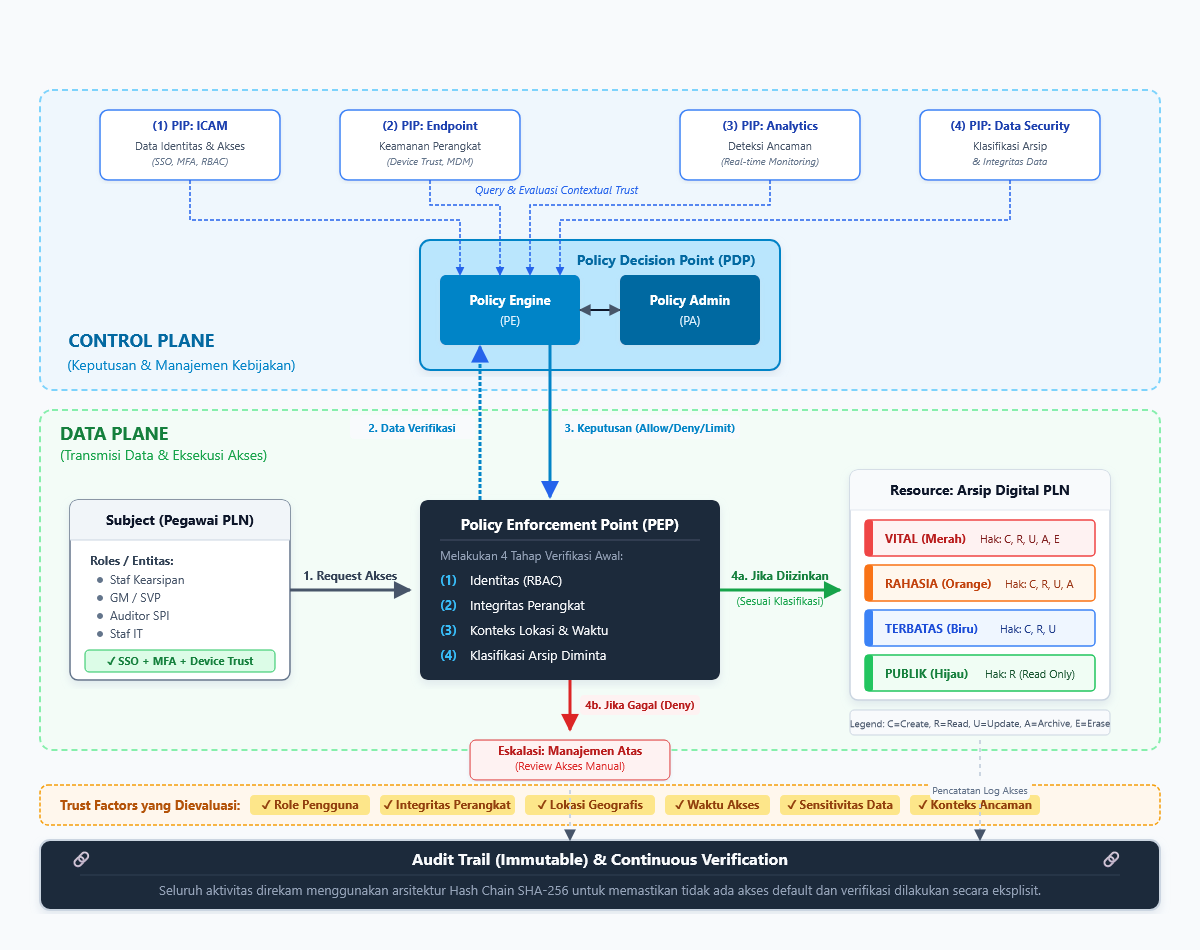
\includegraphics[width=0.98\textwidth,height=0.52\textheight,keepaspectratio]{nist.png}
\caption{Model \textit{Zero Trust} untuk Keamanan Arsip Digital PLN -- Arsitektur Lengkap dengan \textit{Control Plane} dan \textit{Data Plane}\\
\small Sumber: NIST SP 800-207 \textit{Zero Trust Architecture}, diadaptasi untuk konteks PLN.}
\label{fig:zero-trust-pln}
\end{figure}

\small Gambar \ref{fig:zero-trust} menampilkan General \textit{Zero Trust Architecture} Reference dari NIST yang menggambarkan seluruh komponen logis arsitektur \textit{Zero Trust}. Diagram ini terbagi menjadi dua bidang: \textit{Control Plane} yang menangani keputusan kebijakan, dan \textit{Data Plane} yang menangani transmisi data aktual. Subject (pengguna/perangkat) mengajukan permintaan akses melalui Policy Enforcement Point (PEP), yang kemudian meneruskan data verifikasi ke Policy Decision Point (PDP) -- yang terdiri dari Policy Engine (PE) dan Policy Administrator (PA). PDP meminta data kontekstual dari Policy Information Points (PIPs) yang mencakup ICAM (identitas), Endpoint Security, Security Analytics, dan Data Security. Berdasarkan evaluasi ini, PDP mengembalikan keputusan \textit{allow/deny/limit} kepada PEP, yang kemudian membolehkan atau menolak akses ke Resource. Perhatikan bahwa setiap alur diberi label (I, S, R) menunjukkan verifikasi berkelanjutan, bukan sekadar autentikasi satu kali.

\small Gambar \ref{fig:zero-trust-pln} mengadaptasi arsitektur \textit{Zero Trust} NIST (Gambar 3.4) ke dalam konteks spesifik keamanan arsip digital PLN dengan arsitektur lengkap yang terdiri dari \textit{Control Plane} (keputusan kebijakan) dan \textit{Data Plane} (transmisi data). Pada \textit{Control Plane}, Policy Engine (PE) dan Policy Administrator (PA) bekerja sama untuk mengevaluasi dan mengelola kebijakan akses. PE menerima data verifikasi dari PEP dan melakukan query ke empat Policy Information Points (PIPs): (1) PIP: ICAM untuk data identitas dan akses (SSO, MFA, RBAC), (2) PIP: Endpoint untuk keamanan perangkat (Device Trust, MDM), (3) PIP: Analytics untuk deteksi ancaman real-time, dan (4) PIP: Data Security untuk klasifikasi dan integritas data arsip.

Pada \textit{Data Plane}, Subject (pegawai PLN dengan berbagai role: Staf Kearsipan, GM/SVP, Auditor SPI, Staf IT) yang telah terautentikasi melalui SSO + MFA + Device Trust mengajukan permintaan akses ke Policy Enforcement Point (PEP). PEP melakukan 4 tahap verifikasi awal: (1) identitas melalui RBAC, (2) integritas perangkat, (3) konteks lokasi dan waktu, serta (4) klasifikasi arsip yang diminta. Data verifikasi ini dikirim ke \textit{Control Plane} untuk evaluasi mendalam.

Berdasarkan respons dari PIPs, PE mengembalikan keputusan (Allow/Deny/Limit) ke PEP. Jika diizinkan, PEP memberikan akses ke Resource berupa arsip digital PLN yang terklasifikasi berdasarkan tingkat keamanan: Vital (merah), Rahasia (orange), Terbatas (biru), dan Publik (hijau). Setiap klasifikasi memiliki hak akses berbeda (Create/Read/Update/Archive/Erase). Jika verifikasi gagal, akses ditolak dan dieskalasi ke Manajemen Atas untuk review manual.

Seluruh aktivitas dicatat dalam Audit Trail immutable dengan hash chain SHA-256, memungkinkan verifikasi berkelanjutan (\textit{Continuous Verification}) sesuai prinsip \textit{Zero Trust} NIST. \textit{Trust factors} yang dievaluasi mencakup: role pengguna, integritas perangkat, lokasi geografis, waktu akses, sensitivitas data, dan konteks ancaman. Pendekatan ini sangat relevan untuk PLN dengan infrastruktur tersebar di seluruh Indonesia, memastikan bahwa tidak ada akses default dan setiap permintaan diverifikasi secara eksplisit berdasarkan konteks \textit{real-time}.

\needspace{4\baselineskip}

\section{Integrasi GCG BUMN (TARIF)}

TARIF adalah akronim dari lima prinsip tata kelola yang menjadi tolok ukur kinerja BUMN sebagaimana diatur dalam Permen BUMN PER-2/MBU/03/2023 tentang Pedoman GCG Signifikan BUMN. Kelima prinsip ini memiliki implikasi langsung terhadap kebijakan keamanan arsip digital. Tabel \ref{tab:pemetaan-gcg} merangkum implementasi setiap prinsip TARIF dalam konteks kebijakan keamanan arsip:

\begingroup
\small
\begin{xltabular}{\textwidth}{@{} l X @{}}
\caption{Pemetaan Prinsip GCG ke Kebijakan Keamanan Arsip}
\label{tab:pemetaan-gcg}\\
\toprule
\textbf{Prinsip TARIF} & \textbf{Implementasi dalam Kebijakan Arsip} \\
\midrule
\endfirsthead

\multicolumn{2}{@{}l}{\small\textit{Lanjutan Tabel \thetable}}\\
\toprule
\textbf{Prinsip TARIF} & \textbf{Implementasi dalam Kebijakan Arsip} \\
\midrule
\endhead

\bottomrule
\endfoot

Transparansi & Audit trail dapat diakses Auditor Internal/Eksternal sesuai kewenangan \\
Akuntabilitas & RACI digital jelas; setiap aksi terikat identitas dan TTE \\
Responsibilitas & Kepatuhan PP 71/2019 \& Perka ANRI 6/2021 wajib diuji berkala \\
Independensi & Unit Kearsipan berwenang tolak arsip tidak memenuhi standar metadata \\
\textit{Fairness} & Akses berbasis \textit{need-to-know}, tidak diskriminatif, ada mekanisme banding \\
\end{xltabular}
\endgroup

Berikut penjelasan detail dari kelima prinsip TARIF dan implementasinya dalam kebijakan keamanan arsip digital:

\begin{itemize}[leftmargin=*]
    \item Transparansi (Transparency) -- Kebijakan keamanan arsip harus dapat diakses dan dipahami oleh seluruh pemangku kepentingan yang berkepentingan, termasuk auditor eksternal. Hal ini tercermin dalam keterbukaan audit trail dan prosedur akses.
    \item Akuntabilitas (Accountability) -- Setiap aksi terhadap arsip harus dapat dipertanggungjawabkan kepada individu dan peran yang spesifik. Hal ini diterjemahkan melalui matriks RACI digital dan penggunaan Tanda Tangan Elektronik Tersertifikasi (TTE).
    \item Responsibilitas (Responsibility) -- Organisasi memiliki kewajiban untuk mematuhi regulasi kearsipan nasional (PP 71/2019, Perka ANRI 6/2021) dan membuktikan kepatuhan tersebut secara berkala melalui audit internal dan eksternal.
    \item Independensi (Independence) -- Unit Kearsipan dan fungsi pengawasan harus memiliki kewenangan untuk menolak arsip yang tidak memenuhi standar metadata, tanpa tekanan dari pihak manapun. Hal ini menjamin integritas sistem kearsipan secara keseluruhan.
    \item Kewajaran (\textit{Fairness}) -- Kebijakan akses harus berbasis prinsip \textit{need-to-know} dan tidak diskriminatif, dengan mekanisme banding bagi pengguna yang merasa hak aksesnya tidak sesuai.
\end{itemize}

\needspace{4\baselineskip}

\section{Langkah-Langkah Perumusan Kebijakan Keamanan}
Merumuskan kebijakan keamanan arsip bukan aktivitas satu kali, melainkan proses tata kelola yang berkelanjutan. Bagi Manajemen Atas, tahapan berikut harus dipastikan terlaksana:

\begin{enumerate}[leftmargin=*]
    \item Analisis Risiko Kearsipan. Sebelum menulis kebijakan, lakukan identifikasi risiko keamanan arsip digital di unit Anda -- apa ancaman terbesar (kebocoran internal, serangan siber, bencana alam, kelalaian pegawai?), kemungkinan terjadinya, dan dampaknya terhadap bisnis. Hasil analisis risiko ini menjadi dasar prioritas kebijakan. Tanpa analisis risiko, kebijakan menjadi tidak berbasis bukti.
    \item Penyusunan Draf oleh TimLintas. Tim Kearsipan bersama IT Governance dan Legal menyusun draf kebijakan. Gunakan template kerangka (Bagian \ref{sec:template-kebijakan}) sebagai acuan minimal.
    \item Konsultasi Internal. Draf dikonsultasikan dengan unit terkait (Legal, IT, HR, Unit Kearsipan). Pastikan setiap prinsip TARIF terakomodasi dan tidak ada konflik kepentingan antar-unit.
    \item Penetapan dan Pengesahan. Manajemen Atas mengesahkan kebijakan, menetapkan tanggal efektif berlaku, dan menunjuk penanggung jawab implementasi.
    \item Sosialisasi dan Implementasi. Pastikan seluruh pihak terkait memahami kebijakan baru. Tetapkan timeline implementasi bertahap dan kriteria keberhasilan.
    \item Review dan Pembaruan Berkala. Sesuai siklus PDCA (Gambar 3.1), kebijakan harus ditinjau minimal tahunan atau segera setelah terjadi insiden keamanan arsip yang signifikan.
\end{enumerate}

\needspace{4\baselineskip}

\section{Template Kerangka Kebijakan Keamanan Arsip Digital}
\label{sec:template-kebijakan}
Berikut adalah kerangka kebijakan yang dapat digunakan oleh Manajemen Atas sebagai acuan minimal untuk menilai kecukupan draf dari tim. Setiap klausul harus dikembangkan sesuai konteks dan kebutuhan spesifik unit masing-masing.

\begin{plnbox}[Klausul 1: Ruang Lingkup dan Tujuan]
Kebijakan ini berlaku untuk seluruh arsip digital yang dikelola oleh [Nama Unit]. Tujuannya adalah menjamin keamanan, integritas, keterlacakan, dan ketersediaan arsip digital sepanjang siklus hidupnya, sesuai dengan regulasi yang berlaku.
\end{plnbox}

\begin{plnbox}[Klausul 2: Kontrol Akses (merujuk Pilar 1)]
Akses terhadap arsip digital diberikan berdasarkan peran (RBAC) sesuai matriks yang ditetapkan dalam lampiran. Prinsip \textit{least privilege} wajib diterapkan. Pemberian hak akses baru memerlukan persetujuan [Jabatan], dan pencabutan akses dilakukan paling lambat [waktu] setelah perubahan status kepegawaian.
\end{plnbox}

\begin{plnbox}[Klausul 3: Audit Trail dan Keterlacakan (merujuk Pilar 2)]
Setiap akses, perubahan, dan persetujuan terhadap arsip [Klasifikasi: Rahasia/Vital] wajib dicatat dalam log audit yang memenuhi standar 14 field metadata (lihat lampiran). Log audit bersifat immutable dan disimpan terpisah dari sistem produksi selama minimal [periode retensi, sesuai retensi arsipnya].
\end{plnbox}

\begin{plnbox}[Klausul 4: Backup dan Pemulihan (merujuk Pilar 4)]
Arsip digital wajib dibackup sesuai strategi 3-2-1. Target RTO dan RPO ditetapkan berdasarkan klasifikasi arsip (lihat matriks RTO/RPO). Uji simulasi pemulihan dilakukan minimal setiap 6 bulan dengan dokumentasi hasil dan rekomendasi perbaikan.
\end{plnbox}

\begin{plnbox}[Klausul 5: Peran dan Tanggung Jawab]
Matriks RACI (Responsible, Accountable, Consulted, Informed) disusun sebagai lampiran dokumen kebijakan ini. Sebagai panduan minimal: Accountable untuk kebijakan keamanan arsip adalah GM/SVP level unit; Responsible adalah Kepala Unit Kearsipan bersama Kepala IT Governance; Consulted meliputi Legal, HR, dan SPI; serta Informed mencakup seluruh pegawai yang mengakses arsip digital. Kebijakan ini merupakan bagian dari ISMS organisasi yang berlaku.
\end{plnbox}

\begin{plnbox}[Klausul 6: Kepatuhan dan Peninjauan]
Kepatuhan terhadap kebijakan ini dievaluasi melalui audit internal minimal [frekuensi]. Kebijakan ditinjau oleh [Jabatan] minimal setiap [periode] atau segera setelah insiden keamanan arsip yang signifikan.
\end{plnbox}

\begin{plnbox}[Ringkasan untuk Manajemen Atas -- Bab 3]
Kebijakan keamanan arsip adalah payung hukum yang memberikan legitimasi dan keberlanjutan bagi seluruh mekanisme keamanan (RBAC, audit trail, backup). Tiga pesan kunci: (1) kebijakan harus terintegrasi dengan ISMS organisasi (ISO 27001:2022), bukan dokumen yang berdiri sendiri; (2) tiga prinsip fundamental -- \textit{Least Privilege}, \textit{Defense in Depth}, dan \textit{Zero Trust} -- harus tercermin dalam setiap klausul kebijakan; dan (3) kebijakan yang tidak ditinjau secara berkala (minimal tahunan) akan menjadi usang dan kehilangan kekuatan hukumnya. Manajemen Atas adalah penandatangan dan penanggung jawab utama kebijakan ini.
\end{plnbox}

\needspace{4\baselineskip}

\section{Aktivitas Workshop (30 Menit)}
\begin{enumerate}[leftmargin=*]
    \item Susun draf klausul kebijakan keamanan arsip (maks. 2 halaman).
    \item Petakan minimal 3 kontrol ISO 27001 yang relevan dengan unit Anda.
    \item Integrasikan 1 klausul pendukung prinsip TARIF.
\end{enumerate}

\begin{outputbox}
\textbf{Portofolio 3 (Pilar 3: Kebijakan Keamanan):} Rancangan Kebijakan Keamanan Arsip Terintegrasi ISMS. Dinilai berdasarkan kemampuan peserta merumuskan kebijakan keamanan yang terintegrasi dengan ISMS organisasi, keselarasan ISO 27001, kejelasan prinsip \textit{Zero Trust}/\textit{Least Privilege}, dan integrasi GCG BUMN.
\end{outputbox}

% ============================================================
\chapter{Sistem Backup \& Disaster Recovery Terintegrasi}
(Kriteria Penilaian 4.4.4 -- Target Kompetensi 4)
% ============================================================

Bab ini mendukung pencapaian Pilar 4: Pemulihan Data -- peserta mampu merancang sistem backup dan disaster recovery terintegrasi. Keamanan arsip tidak lengkap tanpa jaminan ketersediaan pasca-gangguan. Fokus pada level kebijakan: strategi, target pemulihan, dan kesiapan organisasi.

Mengapa bab ini berurutan setelah Kebijakan Keamanan? Kebijakan keamanan (Pilar 3) menetapkan apa yang harus dilindungi dan bagaimana standar perlindungannya. Namun, kebijakan tanpa mekanisme pemulihan (backup/DR) hanya mengelola risiko secara parsial -- arsip yang sangat aman tetapi tidak dapat dipulihkan saat terjadi bencana sama buruknya dengan arsip yang tidak aman. ISO 27001:2022 secara eksplisit mengklasifikasikan backup sebagai kontrol wajib (A.8.13 Information Backup)\footnote{ISO/IEC 27001:2022, cl. A.8.13.}, dan ISO 22301:2019\footnote{ISO 22301:2019, \textit{Business Continuity Management Systems -- Requirements}, 2nd ed. (Geneva: ISO, 2019).} mewajibkan organisasi memiliki rencana kelangsungan bisnis. Backup dan Disaster Recovery (Pilar 4) melengkapi tiga pilar sebelumnya dengan menjamin bahwa arsip yang dilindungi oleh RBAC (Pilar 1), dicatat oleh audit trail (Pilar 2), dan diatur oleh kebijakan (Pilar 3) juga tersedia saat dibutuhkan -- bahkan dalam kondisi terburuk sekalipun.

\needspace{4\baselineskip}

\section{Strategi Backup 3-2-1 untuk Arsip PLN}

Strategi 3-2-1 adalah standar minimum industri yang direkomendasikan oleh US-CERT/CISA untuk melindungi data dari kehilangan. Angka ``3-2-1'' merujuk pada tiga aturan: minimal 3 salinan data, tersimpan pada sedikitnya 2 jenis media yang berbeda, dan sedikitnya 1 salinan disimpan di lokasi terpisah (offsite). Dalam konteks PLN, strategi ini diterapkan untuk menjamin bahwa kehilangan data akibat kegagalan perangkat, bencana lokasi, atau serangan siber dapat diminimalkan, karena tidak ada satu pun titik kegagalan tunggal yang dapat mengkompromikan seluruh salinan secara bersamaan. Gambar \ref{fig:backup-diagram} mengilustrasikan penerapan strategi ini di lingkungan PLN.

%% ============================================================
%% GAMBAR 4.1 — Diagram Strategi Backup 3-2-1 (Custom Image)
%% Sumber: Gambar kustom pengguna (321_rule.png)
%% Referensi akademis: US-CERT/CISA Data Backup Options
%% ============================================================

\begin{figure}[H]
\centering
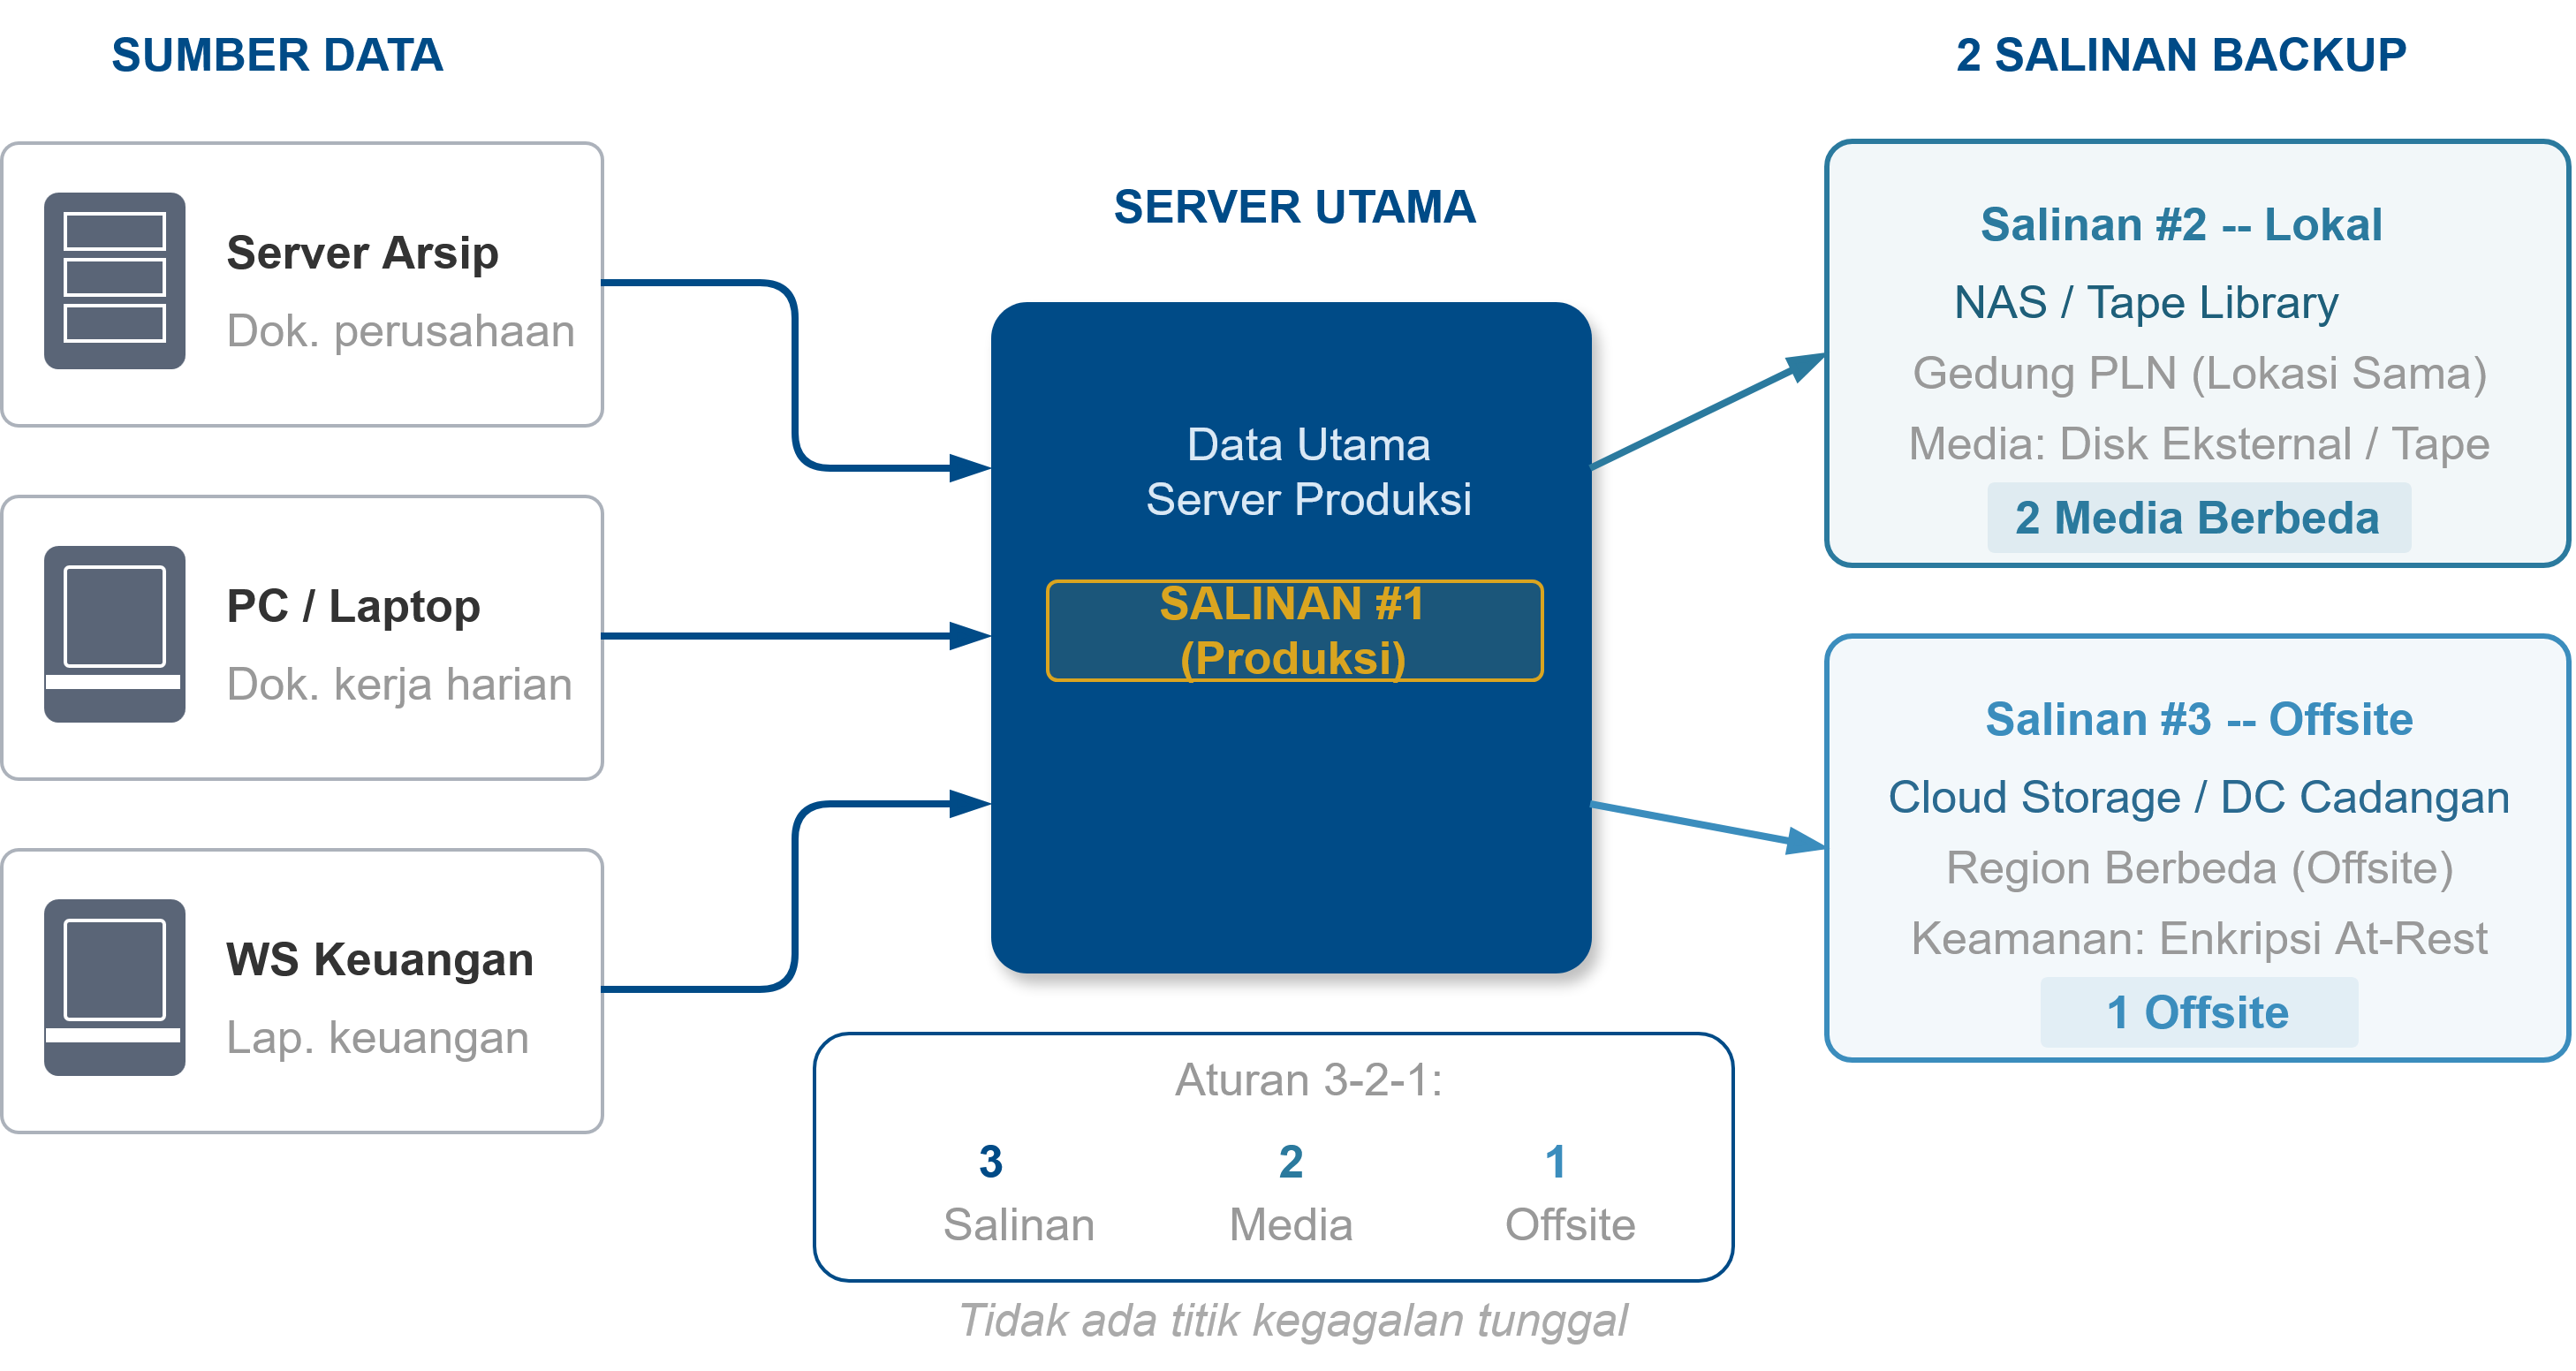
\includegraphics[width=0.80\textwidth]{321_rule.png}
\caption{Strategi Backup 3-2-1 untuk Arsip Digital PLN -- 3 Salinan, 2 Media, 1 Offsite\\
\small Sumber: US-CERT/CISA.}
\label{fig:backup-diagram}
\end{figure}

\small Gambar \ref{fig:backup-diagram} mengilustrasikan penerapan strategi 3-2-1 backup rule yang direkomendasikan oleh US-CERT/CISA dalam konteks kearsipan digital PLN. Pada sisi kiri, terdapat tiga sumber data: Server Arsip (dokumen perusahaan), PC/Laptop Staf (dokumen kerja harian), dan Workstation Keuangan (laporan keuangan) yang seluruhnya terhubung ke Data Utama (server produksi) di tengah. Dari server utama, data direplikasi ke dua lokasi backup: (1) Salinan \#2 -- Lokal yang disimpan pada NAS/Tape Library dalam gedung PLN yang sama menggunakan media disk eksternal atau tape; dan (2) Salinan \#3 -- Offsite yang disimpan pada Cloud Storage atau Data Center cadangan di region berbeda. Prinsip 3-2-1 menjamin bahwa kehilangan data akibat kegagalan perangkat, bencana lokasi, atau serangan siber dapat diminimalkan secara signifikan, karena tidak ada satu pun titik kegagalan tunggal yang dapat mengkompromikan seluruh salinan data secara bersamaan.

Kebijakan wajib mencantumkan jadwal backup otomatis, enkripsi \textit{at-rest/in-transit}, dan verifikasi integritas pasca-backup.

\needspace{4\baselineskip}

\section{Penetapan RTO \& RPO Berbasis Criticality}

\small Strategi backup 3-2-1 pada Bagian 4.1 menjawab pertanyaan ``bagaimana'' data arsip dilindungi -- yaitu melalui replikasi ke berbagai media dan lokasi. Namun, strategi backup saja tidak cukup; Manajemen Atas juga harus menetapkan ``seberapa cepat'' sistem harus pulih dan ``seberapa banyak data yang boleh hilang'' ketika gangguan terjadi. Dua pertanyaan inilah yang dijawab oleh Recovery Time Objective (RTO) dan Recovery Point Objective (RPO).

Penetapan RTO dan RPO bukanlah keputusan teknis semata, melainkan keputusan strategis yang harus diambil oleh Manajemen Atas berdasarkan dua pertimbangan utama. Pertama, pertimbangan tingkat kepentingan arsip: dokumen seperti kontrak pembangkit listrik atau laporan keuangan teraudit memiliki dampak yang jauh lebih besar jika hilang dibandingkan dengan surat edaran internal, sehingga membutuhkan target pemulihan yang lebih ketat. Kedua, pertimbangan keseimbangan biaya dan risiko: menetapkan RTO dan RPO yang terlalu agresif untuk seluruh arsip akan mengakibatkan pembengkakan biaya infrastruktur tanpa proporsi manfaat yang sepadan. Sebaliknya, target yang terlalu longgar berarti PLN harus menerima risiko downtime yang lebih lama dan potensi kehilangan data yang lebih besar -- sebuah risiko yang dapat berujung pada sanksi regulasi, kerugian finansial, atau gangguan pelayanan publik.

Bagian ini membahas konsep RTO dan RPO secara visual melalui diagram timeline (Gambar \ref{fig:rto-rpo}), kemudian menghubungkannya dengan klasifikasi keamanan arsip PLN sebagaimana diatur dalam Perdir 0037.P/DIR/2022 untuk menghasilkan target pemulihan yang proporsional dan terukur.

%% ============================================================
%% GAMBAR 4.2 — RTO vs RPO Timeline
%% File: gambar/RTO_RPO_Timeline.png (dari SVG: RTO_RPO_Timeline.svg)
%% ============================================================

\begin{figure}[H]
\centering
\resizebox{0.80\textwidth}{!}{%
\begin{tikzpicture}
\definecolor{avail}{RGB}{26,58,92}
\definecolor{disaster}{RGB}{192,57,43}
\definecolor{recovered}{RGB}{39,174,96}

% Solid portion: Available
\draw[avail, line width=2.5pt, -{Stealth[length=6pt]}] (0,3) -- (7.0,3);
% Dashed portion: Not Available
\draw[disaster, line width=2.5pt, dashed] (7.2,3) -- (10.0,3);
% Solid after recovery
\draw[avail, line width=2.5pt, -{Stealth[length=5pt]}] (10.2,3) -- (12.0,3);
\node[font=\scriptsize\itshape, text=gray] at (11.5,2.5) {time};

% Backup markers
\draw[avail, line width=1.5pt] (1.5,2.7) -- (1.5,3.3);
\node[font=\scriptsize\itshape, text=avail, anchor=north] at (1.5,2.65) {Backup};
\draw[avail, line width=1.5pt] (3.0,2.7) -- (3.0,3.3);
\node[font=\scriptsize\itshape, text=avail, anchor=north] at (3.0,2.65) {Backup};

% Recovery Point marker
\draw[avail, line width=1.5pt] (5.0,2.7) -- (5.0,3.3);
\node[font=\scriptsize\itshape, text=avail, anchor=south] at (5.0,3.35) {Recovery Point};

% Disaster marker with lightning bolt
\draw[disaster, line width=2pt] (7.2,2.5) -- (7.2,3.3);
% Lightning bolt (simple TikZ polygon)
\fill[disaster] (7.0,4.0) -- (7.3,3.5) -- (7.1,3.5) -- (7.4,2.8) -- (7.1,3.15) -- (7.3,3.15) -- cycle;
\node[font=\small\bfseries\itshape, text=disaster] at (7.2,4.25) {Disaster};

% Recovered marker
\draw[recovered, line width=2pt] (10.2,2.7) -- (10.2,3.3);
\node[font=\scriptsize\itshape, text=recovered, anchor=south] at (10.2,3.35) {Recovered};

% ---- RPO BRACKET ----
\draw[avail, line width=1.2pt] (3.0,1.4) -- (5.0,1.4);
\draw[avail, line width=1.2pt] (3.0,1.1) -- (3.0,1.7);
\draw[avail, line width=1.2pt] (5.0,1.1) -- (5.0,1.7);
\fill[avail] (3.15,1.4) -- (3.0,1.2) -- (3.0,1.6) -- cycle;
\fill[avail] (4.85,1.4) -- (5.0,1.2) -- (5.0,1.6) -- cycle;
\node[avail, font=\small\bfseries] at (4.0,1.0) {RPO};
\node[avail, font=\tiny, anchor=north] at (4.0,0.8) {Recovery Point Objective};

% ---- RTO BRACKET ----
\draw[disaster, line width=1.2pt, dashed] (7.2,0.0) -- (10.2,0.0);
\draw[disaster, line width=1.2pt] (7.2,-0.3) -- (7.2,0.3);
\draw[disaster, line width=1.2pt] (10.2,-0.3) -- (10.2,0.3);
\fill[disaster] (7.35,0.0) -- (7.2,-0.2) -- (7.2,0.2) -- cycle;
\fill[disaster] (10.05,0.0) -- (10.2,-0.2) -- (10.2,0.2) -- cycle;
\node[disaster, font=\small\bfseries] at (8.7,-0.4) {RTO};
\node[disaster, font=\tiny, anchor=north] at (8.7,-0.6) {Recovery Time Objective};

% ---- LEGEND (3 items, vertical, centered below) ----
\fill[gray!8, rounded corners=2pt] (3.0,-2.6) rectangle (9.0,-1.1);
% Item 1: Available
\draw[avail, line width=2pt] (3.3,-1.35) -- (4.3,-1.35);
\node[font=\tiny, anchor=west, text=avail] at (4.45,-1.35) {Available (Sistem Beroperasi)};
% Item 2: Not Available
\draw[disaster, line width=2pt, dashed] (3.3,-1.85) -- (4.3,-1.85);
\node[font=\tiny, anchor=west, text=disaster] at (4.45,-1.85) {Not Available (Sistem Lumpuh)};
% Item 3: Recovered
\draw[recovered, line width=2pt] (3.3,-2.35) -- (4.3,-2.35);
\node[font=\tiny, anchor=west, text=recovered] at (4.45,-2.35) {Recovered};

\end{tikzpicture}%
}
\caption{Timeline RTO dan RPO -- RPO diukur dari backup terakhir ke titik bencana; RTO diukur dari bencana ke pemulihan sistem\\
\small Sumber: NIST SP 800-34 Rev.~1.}
\label{fig:rto-rpo}
\end{figure}

\small Gambar \ref{fig:rto-rpo} mengilustrasikan dua metrik kritis dalam perencanaan disaster recovery. Garis kontinu menandakan operasional normal dengan backup berkala; garis putus-putus menandakan periode \textit{Not Available} setelah bencana. \textit{RPO} (Recovery Point Objective) mengukur celah waktu antara backup terakhir dan bencana, yang menentukan seberapa banyak data berpotensi hilang. \textit{RTO} (Recovery Time Objective) mengukur durasi lumpuh total sistem, yang menentukan seberapa cepat operasional harus dipulihkan. Kedua metrik ini adalah keputusan bisnis strategis, bukan parameter teknis semata.

Mengapa Manajemen Atas perlu memahami RTO dan RPO? Kedua metrik ini bukan sekadar parameter teknis -- melainkan keputusan bisnis strategis yang memiliki implikasi langsung terhadap biaya operasional dan manajemen risiko PLN. Menetapkan RTO 1 jam dan RPO 15 menit untuk seluruh arsip akan sangat mahal dan tidak efisien, karena tidak semua arsip memiliki tingkat kepentingan yang sama. Oleh karena itu, penetapan RTO/RPO harus proporsional dengan klasifikasi keamanan arsip sebagaimana diatur dalam Perdir 0037.P/DIR/2022. Tabel \ref{tab:rto-rpo} merangkum target pemulihan yang direkomendasikan berdasarkan tingkat kepentingan:

\begingroup
\small
\begin{xltabular}{\textwidth}{@{} >{\raggedright\arraybackslash}p{2.2cm} P{2.5cm} P{2.5cm} X @{}}
\caption{Target Pemulihan (RTO/RPO) Berdasarkan Klasifikasi Arsip}
\label{tab:rto-rpo}\\
\renewcommand{\arraystretch}{1.5}
\textcolor{white}{\textbf{Klasifikasi}} & \textcolor{white}{\textbf{RTO}} & \textcolor{white}{\textbf{RPO}} & \textcolor{white}{\textbf{Strategi Prioritas}} \\
\midrule
\endfirsthead

\multicolumn{4}{@{}l}{\small\textit{Lanjutan Tabel \thetable}}\\
\textcolor{white}{\textbf{Klasifikasi}} & \textcolor{white}{\textbf{RTO}} & \textcolor{white}{\textbf{RPO}} & \textcolor{white}{\textbf{Strategi Prioritas}} \\
\midrule
\endhead

\bottomrule
\endfoot

Vital & $< 4$ jam & $< 1$ jam & \textit{Mirror site} aktif, \textit{failover} otomatis, replikasi waktu nyata \\
Rahasia & $< 12$ jam & $< 4$ jam & Backup harian terenkripsi, \textit{restore} manual teruji \\
Internal/ Publik & $< 24$ jam & $< 12$ jam & Backup mingguan, arsip dingin (cold storage) \\
\end{xltabular}
\endgroup

\needspace{4\baselineskip}

\section{\textit{Business Continuity Plan} (BCP) Kearsipan}

\small Bagian 4.2 telah membahas penetapan RTO dan RPO sebagai target pemulihan yang proporsional dengan tingkat kepentingan arsip. Namun, target pemulihan yang telah ditetapkan tidak akan berarti apa-apa tanpa sebuah rencana terstruktur yang mengatur bagaimana organisasi harus bertindak ketika gangguan benar-benar terjadi. \textit{Business Continuity Plan} (BCP) adalah rencana tersebut -- sebuah dokumen strategis yang memastikan PLN dapat tetap menjalankan fungsi bisnis kritis, termasuk pengelolaan arsip digital, meskipun menghadapi bencana besar.

Dalam konteks kearsipan PLN, BCP menjawab pertanyaan yang lebih luas dari sekadar teknis backup: ``Jika data center utama mengalami kegagalan total, apakah kontrak pembangkit yang sedang dalam proses tender masih bisa diakses oleh panitia? Jika server arsip diretas oleh \textit{ransomware}, apakah laporan keuangan teraudit yang dibutuhkan OJK masih tersedia untuk diaudit? Jika bencana alam melumpuhkan kantor pusat, apakah dokumen RUPS dapat direproduksi untuk pemegang saham?'' Pertanyaan-pertanyaan ini bersifat manajerial, bukan teknis -- dan jawabannya harus disiapkan oleh Manajemen Atas melalui penyusunan BCP yang komprehensif.

Secara internasional, kerangka BCP yang paling banyak diadopsi adalah ISO 22301:2019 (Security and resilience -- Business continuity management systems). Standar ini mensyaratkan organisasi untuk menjalankan siklus manajemen kelangsungan bisnis yang mencakup analisis dampak, perancangan solusi, implementasi, pengujian, dan pemeliharaan berkelanjutan. Bagian ini membahas siklus BCP tersebut secara visual (Gambar \ref{fig:bcp-lifecycle}), kemudian memfokuskan pada tahap \textit{Business Impact Analysis} (BIA) yang menjadi tanggung jawab langsung Manajemen Atas dalam menentukan prioritas pemulihan arsip.

%% ============================================================
%% GAMBAR 4.3 — BCP Lifecycle (Custom Image)
%% ============================================================
\begin{figure}[H]
\centering
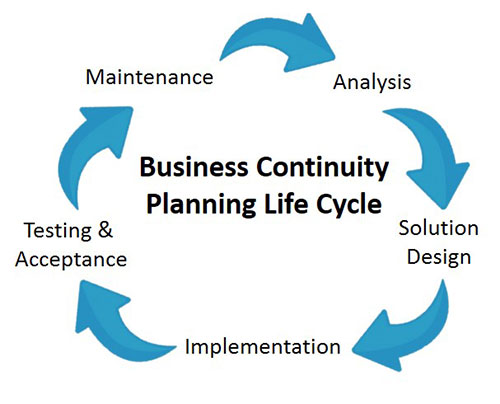
\includegraphics[width=0.50\textwidth,height=0.30\textheight,keepaspectratio]{gambar/BCP_Lifecycle_Custom.png}
\caption{Siklus Hidup \textit{Business Continuity Plan} (BCP) -- Lima Fase Iteratif ISO 22301:2019\\
\small Sumber: ISO 22301:2019.}
\label{fig:bcp-lifecycle}
\end{figure}

\small Gambar \ref{fig:bcp-lifecycle} menampilkan siklus hidup BCP yang terdiri dari 5 fase iteratif searah jarum jam. Fase \textit{Analysis} (berisi BIA) adalah tanggung jawab langsung Manajemen Atas untuk menetapkan prioritas pemulihan arsip berdasarkan dampak bisnis. Kelima fase tersebut adalah: (1)~Maintenance -- pemeliharaan dan pembaruan rencana; (2)~Analysis -- identifikasi proses kritis, penilaian risiko, dan penetapan RTO/RPO; (3)~Solution Design -- perumusan strategi backup dan \textit{failover}; (4)~Implementation -- penyusunan SOP dan penunjukan tim respons; serta (5)~Testing \& Acceptance -- simulasi pemulihan dan umpan balik ke fase Maintenance.

\noindent Panah searah jarum jam menghubungkan kelima fase secara iteratif, menandakan bahwa BCP bukan proyek satu kali selesai melainkan siklus perbaikan berkelanjutan yang sejalan dengan prinsip ISO 22301:2019. Kebijakan DR kearsipan PLN harus mencakup seluruh fase dalam siklus ini. Khusus untuk arsip vital, diperlukan prosedur \textit{fallback} yang jelas ketika sistem elektronik mengalami \textit{downtime} lebih dari 4 jam, termasuk mekanisme pengelolaan arsip manual sementara.

Kebijakan DR harus mencakup:
\begin{enumerate}[leftmargin=*]
    \item Prosedur \textit{fallback} digital/manual saat sistem lumpuh $>4$ jam.
    \item Prioritas pemulihan: Vital $\rightarrow$ Rahasia $\rightarrow$ Internal.
    \item Jadwal simulasi pemulihan minimal 6 bulan sekali dengan dokumentasi hasil evaluasi.
    \item Mekanisme komunikasi krisis dan eskalasi ke manajemen puncak.
\end{enumerate}

\needspace{4\baselineskip}

\subsection{Analisis Dampak Bisnis (BIA) untuk Arsip Digital}
BIA adalah tahap paling kritis dalam perancangan BCP/DR -- dan merupakan kegiatan yang secara langsung menjadi tanggung jawab Manajemen Atas. BIA menjawab pertanyaan strategis: ``Jika arsip X tidak dapat diakses selama Y jam, apa dampaknya terhadap operasional, keuangan, reputasi, dan kepatuhan regulasi?'' Tanpa BIA, penetapan RTO/RPO hanyalah tebakan tanpa dasar bisnis. Tabel \ref{tab:bia} menyajikan template BIA ringkas yang memetakan empat kategori klasifikasi arsip terhadap contoh arsip di PLN serta dampak operasional dan regulasinya masing-masing.

\begingroup
\small
\begin{xltabular}{\textwidth}{@{} >{\raggedright\arraybackslash}p{1.5cm} X X X @{}}
\caption{Template BIA Ringkas untuk Arsip Digital PLN}
\label{tab:bia}\\
\renewcommand{\arraystretch}{1.6}
\textcolor{white}{\textbf{Kategori}} & \textcolor{white}{\textbf{Contoh Arsip di PLN}} & \textcolor{white}{\textbf{Dampak Operasional}} & \textcolor{white}{\textbf{Dampak Regulasi}} \\
\midrule
\endfirsthead

\multicolumn{4}{@{}l}{\small\textit{Lanjutan Tabel \thetable}}\\
\textcolor{white}{\textbf{Kategori}} & \textcolor{white}{\textbf{Contoh Arsip di PLN}} & \textcolor{white}{\textbf{Dampak Operasional}} & \textcolor{white}{\textbf{Dampak Regulasi}} \\
\midrule
\endhead

\bottomrule
\endfoot

Vital & Kontrak pembangkit, laporan keuangan teraudit, dokumen RUPS & Gangguan operasional nasional; potensi kerugian triliunan rupiah & Pelanggaran UU Perseroan; sanksi OJK; ancaman pidana \\
Rahasia & Data pelanggan, dokumen tender, laporan audit & Gangguan layanan regional; potensi kebocoran data pelanggan & Pelanggaran UU PDP; ancaman pidana; denda administratif \\
Terbatas & SOP internal, laporan kinerja unit, surat keputusan & Gangguan operasional unit; penurunan efisiensi & Potensi temuan audit internal \\
Publik & Info publik, laporan tahunan, profil perusahaan & Minimal -- tidak mengganggu operasional & Tidak ada \\
\end{xltabular}
\endgroup

Pertanyaan kunci untuk Manajemen Atas: ``Jika seluruh arsip vital unit ini musnah besok, apakah kita bisa melanjutkan operasional? Berapa kerugian finansial yang ditimbulkan? Apakah kita siap menghadapi pemeriksaan regulator?''

\needspace{4\baselineskip}

\subsection{Langkah-Langkah Perancangan Sistem Backup/DR}
Bagi Manajemen Atas, perancangan sistem backup dan disaster recovery berfokus pada kebijakan, target, dan kesiapan organisasi -- bukan pemilihan teknologi. Tahapan tata kelola berikut harus dipastikan:

\begin{enumerate}[leftmargin=*]
    \item Lakukan BIA. Identifikasi arsip vital dan estimasi dampak ketidaktersediaan. Manajemen Atas menetapkan klasifikasi vital berdasarkan dampak bisnis.
    \item Tetapkan Target RTO/RPO. Berdasarkan hasil BIA, tetapkan target pemulihan yang realistis dan proporsional dengan anggaran yang tersedia. Target yang terlalu agresif tanpa anggaran yang memadai akan menjadi kebijakan di atas kertas.
    \item Tetapkan Strategi Backup. Pastikan tim IT mengimplementasikan strategi 3-2-1. Manajemen Atas menyetujui alokasi anggaran untuk infrastruktur backup (cloud, offsite, enkripsi).
    \item Tetapkan Prosedur \textit{Fallback}. Jika sistem elektronik lumpuh lebih dari 4 jam, bagaimana unit beroperasi? Prosedur \textit{fallback} manual harus ada dan pernah disimulasikan.
    \item Jadwalkan dan Lakukan Simulasi. Manajemen Atas menetapkan jadwal simulasi minimal 6 bulanan dan menghadiri (atau menerima laporan) setiap simulasi. Simulasi yang tidak pernah dilakukan sama saja dengan tidak punya BCP.
\end{enumerate}

\begin{plnbox}[Ringkasan untuk Manajemen Atas -- Bab 4]
Backup dan disaster recovery bukan aktivitas teknis semata -- ini adalah keputusan bisnis strategis yang menentukan apakah PLN dapat terus beroperasi saat terjadi gangguan serius. Tiga pesan kunci: (1) strategi backup 3-2-1 adalah standar minimum yang harus diimplementasikan -- tiga salinan, dua media berbeda, satu offsite; (2) penetapan RTO/RPO harus proporsional dengan klasifikasi arsip -- tidak semua arsip memerlukan pemulihan instan, tetapi arsip vital memerlukan target yang ketat; dan (3) BCP yang tidak pernah diuji melalui simulasi sama saja dengan tidak punya BCP -- Manajemen Atas harus memastikan bahwa uji pemulihan dilakukan minimal setiap 6 bulan.
\end{plnbox}

\needspace{4\baselineskip}

\section{Aktivitas Workshop (30 Menit)}
\begin{enumerate}[leftmargin=*]
    \item Tentukan klasifikasi arsip vital di unit Anda.
    \item Tetapkan target RTO/RPO realistis.
    \item Rancang jadwal backup dan skenario simulasi 6 bulanan.
\end{enumerate}

\begin{outputbox}
\textbf{Portofolio 4 (Pilar 4: Pemulihan Data):} Matriks RTO/RPO + Rencana Backup \& DR. Dinilai berdasarkan kemampuan peserta merancang sistem backup dan disaster recovery terintegrasi, kesesuaian 3-2-1, target realistis, dan kejelasan prosedur \textit{fallback}/simulasi.
\end{outputbox}

% ============================================================
\chapter{Studi Kasus Terintegrasi: Insiden Kebocoran Arsip Kontrak}
(Mengintegrasikan Pilar 1 hingga Pilar 4)
% ============================================================

\needspace{4\baselineskip}

\section{Skenario}
Pada hari Senin pukul 08.00, Manajer Keuangan Unit Bisnis PLN XYZ menemukan bahwa dokumen kontrak jangka panjang dengan vendor strategis telah diunduh oleh 3 orang yang tidak berwenang pada hari Jumat malam pukul 23.45. Dokumen tersebut berstatus Rahasia dan mengandung informasi komersial sensitif. Insiden ini baru terdeteksi setelah 2,5 hari, ketika staf administrasi kebetulan memeriksa log sistem dan menemukan anomali.

\needspace{4\baselineskip}

\section{Analisis Berbasis Empat Pilar Keamanan}

\needspace{4\baselineskip}

\subsection{Pilar 1: Kontrol Akses -- Apakah RBAC Berfungsi?}
\begin{itemize}[leftmargin=*]
    \item Temuan: Ketiga orang yang mengunduh memiliki peran Staf Administrasi. Peran ini seharusnya hanya memiliki hak Read untuk arsip Rahasia, bukan Export/Download.
    \item Akar Masalah: Matriks RBAC tidak membedakan antara View (membaca di layar) dan Export/Download (menyalin ke perangkat lokal). Hak Export diberikan terlalu luas kepada peran yang tidak membutuhkannya.
    \item Tindakan Perbaikan: Revisi matriks RBAC: pisahkan hak Read dan Export. Hak Export untuk arsip Rahasia hanya diberikan melalui prosedur darurat dengan persetujuan atasan langsung.
\end{itemize}

\needspace{4\baselineskip}

\subsection{Pilar 2: Audit Trail -- Apakah Audit Trail Berfungsi?}
\begin{itemize}[leftmargin=*]
    \item Temuan positif: Aksi download tercatat dalam log audit dengan metadata lengkap: siapa, kapan, dari perangkat mana, berapa file yang diunduh. Tanpa audit trail, insiden ini tidak akan pernah terdeteksi.
    \item Temuan negatif: Insiden baru ditemukan 2,5 hari kemudian -- bukan secara waktu nyata. Tidak ada mekanisme peringatan otomatis ketika arsip Rahasia diunduh di luar jam kerja (pukul 23.45), padahal ini adalah pola yang mencurigakan.
    \item Tindakan Perbaikan: Tetapkan aturan alert otomatis untuk event ekspor arsip Rahasia dan Vital di luar jam kerja. Manajemen Atas harus menerima notifikasi untuk event kritis.
\end{itemize}

\needspace{4\baselineskip}

\subsection{Pilar 3: Kebijakan Keamanan -- Apakah Kebijakan Keamanan Memadai?}
\begin{itemize}[leftmargin=*]
    \item Temuan: Kebijakan keamanan arsip yang berlaku tidak mengatur secara spesifik tentang ekspor terkontrol untuk arsip Rahasia. Kebijakan hanya menyebut ``akses dibatasi berdasarkan peran'' tanpa membedakan akses baca dan akses salin.
    \item Temuan tambahan: Kebijakan belum dilakukan peninjauan selama 18 bulan, melampaui periode review tahunan yang direkomendasikan oleh standar ISO 27001.
    \item Tindakan Perbaikan: Revisi kebijakan untuk mencakup klausul ekspor terkontrol, tetapkan jadwal review berkala yang dipatuhi, dan pastikan proses review melibatkan seluruh pemangku kepentingan.
\end{itemize}

\needspace{4\baselineskip}

\subsection{Pilar 4: Pemulihan Data -- Apakah Backup/DR Berfungsi?}
\begin{itemize}[leftmargin=*]
    \item Temuan positif: Arsip kontrak yang dibocorkan masih tersedia di sistem -- integritas data tidak terganggu, sehingga dampak insiden bisa dibatasi pada aspek keamanan, bukan ketersediaan.
    \item Pertanyaan kritis: Jika insiden ini bukan kebocoran tetapi \textit{ransomware} yang mengenkripsi seluruh arsip Rahasia, berapa lama waktu pemulihan? Apakah backup terenkripsi dan terpisah dari jaringan produksi? Kapan terakhir kali simulasi pemulihan dilakukan?
    \item Tindakan Perbaikan: Pastikan strategi 3-2-1 sudah diimplementasikan dan telah diuji melalui simulasi pemulihan dalam 6 bulan terakhir. Verifikasi bahwa backup tidak terjangkau oleh serangan yang sama dengan sistem produksi.
\end{itemize}

\needspace{4\baselineskip}

\section{Pelajaran untuk Manajemen Atas}
Studi kasus ini menunjukkan bahwa keamanan arsip adalah sistem terintegrasi. Kelemahan pada satu pilar akan menetralisasi kekuatan pilar lainnya. RBAC yang tidak cukup detail (Pilar 1) menciptakan celah akses. Tanpa pemantauan audit trail yang aktif (Pilar 2), pelanggaran tidak terdeteksi secara dini. Tanpa kebijakan yang spesifik (Pilar 3), tidak ada dasar hukum untuk menindaklanjuti pelanggaran. Dan tanpa backup yang teruji (Pilar 4), dampak insiden yang lebih besar tidak dapat dipulihkan. Manajemen Atas harus memastikan keempat pilar ini dirancang, diimplementasikan, dan dimonitor secara bersamaan.

\begin{outputbox}
Refleksi Integrasi (Pilar 1 s.d. Pilar 4): Dengan merujuk studi kasus di atas, identifikasi minimal 2 celah keamanan yang berpotensi terjadi di unit Anda. Tentukan tindakan perbaikan untuk setiap pilar (Pilar 1 hingga Pilar 4), siapa yang bertanggung jawab atas implementasinya, dan berapa timeline penyelesaiannya.
\end{outputbox}

% ============================================================
\chapter{Validasi, Portofolio \& Pintu Kendali Manajemen}
% ============================================================

\needspace{4\baselineskip}

\section{Ringkasan Kriteria Penilaian}
Bab ini merupakan titik validasi akhir yang menghubungkan seluruh rancangan yang telah disusun pada Bab 1--5 dengan keputusan pengesahan Manajemen Atas. Tabel berikut memetakan setiap pilar kompetensi ke portofolio wajib yang menjadi bukti kelulusan, disertai fokus penilaian dan bobot yang setara -- menegaskan bahwa keempat pilar bersifat kumulatif dan tidak ada yang dapat diabaikan. Setelah tabel ini, section 6.2 menyajikan rubrik terukur untuk menilai masing-masing portofolio secara objektif, dan section 6.3 menyediakan checklist pengesahan sebelum rancangan diajukan ke Komite Tata Kelola.

\begingroup
\footnotesize
\begin{xltabular}{\textwidth}{@{} >{\centering\arraybackslash}p{1cm} >{\raggedright\arraybackslash}p{3.5cm} X X >{\centering\arraybackslash}p{1cm} @{}}
\caption{Pemetaan Target Kompetensi $\rightarrow$ Kriteria Penilaian $\rightarrow$ Portofolio}\\
\renewcommand{\arraystretch}{1.6}
\textcolor{white}{\textbf{Pilar}} & \textcolor{white}{\textbf{Target Kompetensi}} & \textcolor{white}{\textbf{Portofolio Wajib}} & \textcolor{white}{\textbf{Fokus Penilaian}} & \textcolor{white}{\textbf{Bobot}} \\
\midrule
\endfirsthead

\multicolumn{5}{@{}l}{\small\textit{Lanjutan Tabel \thetable}}\\
\textcolor{white}{\textbf{Pilar}} & \textcolor{white}{\textbf{Target Kompetensi}} & \textcolor{white}{\textbf{Portofolio Wajib}} & \textcolor{white}{\textbf{Fokus Penilaian}} & \textcolor{white}{\textbf{Bobot}} \\
\midrule
\endhead

\bottomrule
\endfoot

Pilar 1 & Merancang skema kontrol akses RBAC terintegrasi dengan sistem kepegawaian & Matriks RBAC + Prosedur Akses & Kejelasan peran, \textit{least privilege}, integrasi HR/SSO, review berkala & 25\% \\
Pilar 2 & Merancang mekanisme audit trail otomatis yang merekam setiap akses dan perubahan arsip & Alur Audit + Template 14 Field & Kelengkapan 4W, immutability, compliance PP 71/2019 dan Perka ANRI 6/2021 & 25\% \\
Pilar 3 & Merumuskan kebijakan keamanan terintegrasi dengan ISMS organisasi & Rancangan Kebijakan Keamanan & Keselarasan ISO 27001, \textit{Zero Trust}, TARIF GCG & 25\% \\
Pilar 4 & Merancang sistem backup dan disaster recovery terintegrasi & Matriks RTO/RPO + Rencana DR & Kesesuaian 3-2-1, target realistis, prosedur \textit{fallback}/simulasi & 25\% \\
\end{xltabular}
\endgroup
Kelulusan: Skor portofolio $\geq 70$, post-test $\geq 65$, submit komitmen tindak lanjut.

\needspace{4\baselineskip}

\section{Rubrik Penilaian Terukur}
Tabel \ref{tab:rubrik-1} hingga Tabel \ref{tab:rubrik-4} memberikan indikator penilaian terukur untuk masing-masing portofolio, agar Manajemen Atas memiliki alat evaluasi yang objektif dan konsisten. Secara berurutan: Tabel \ref{tab:rubrik-1} menilai Matriks RBAC (Pilar 1), Tabel \ref{tab:rubrik-2} menilai Mekanisme Audit Trail (Pilar 2), Tabel \ref{tab:rubrik-3} menilai Kebijakan Keamanan ISMS (Pilar 3), dan Tabel \ref{tab:rubrik-4} menilai Sistem Backup \& DR (Pilar 4).

\begingroup
\small
\begin{xltabular}{\textwidth}{@{} l X @{}}
\caption{Rubrik Penilaian Portofolio 1 -- Pilar 1: Kontrol Akses: Matriks RBAC Terintegrasi}
\label{tab:rubrik-1}\\
\toprule
\textbf{Level} & \textbf{Indikator} \\
\midrule
\endfirsthead

\multicolumn{2}{@{}l}{\small\textit{Lanjutan Tabel \thetable}}\\
\toprule
\textbf{Level} & \textbf{Indikator} \\
\midrule
\endhead

\bottomrule
\endfoot

Kurang (< 50) & Matriks peran tidak lengkap; tidak ada keterkaitan dengan sistem kepegawaian; prinsip \textit{least privilege} tidak diterapkan; tidak ada prosedur \textit{provisioning/de-provisioning}. \\
Cukup (50--69) & Matriks peran lengkap tetapi belum detail; keterkaitan dengan sistem kepegawaian disebutkan secara konseptual; ada prosedur tetapi belum operasional. \\
Baik (70--84) & Matriks peran lengkap dengan pemisahan hak akses yang jelas; prosedur \textit{provisioning/de-provisioning} terhubung dengan siklus hidup kepegawaian; ada mekanisme review berkala. \\
Sangat Baik ($\geq$ 85) & Seluruh indikator Baik terpenuhi, ditambah: validasi \textit{segregation of duties}, mekanisme akses sementara (delegasi, lintas-unit), dan penanganan mutasi darurat sudah tercakup. \\
\end{xltabular}
\endgroup

\begingroup
\small
\begin{xltabular}{\textwidth}{@{} l X @{}}
\caption{Rubrik Penilaian Portofolio 2 -- Pilar 2: Audit Trail: Mekanisme Audit Trail Otomatis}
\label{tab:rubrik-2}\\
\toprule
\textbf{Level} & \textbf{Indikator} \\
\midrule
\endfirsthead

\multicolumn{2}{@{}l}{\small\textit{Lanjutan Tabel \thetable}}\\
\toprule
\textbf{Level} & \textbf{Indikator} \\
\midrule
\endhead

\bottomrule
\endfoot

Kurang (< 50) & Tidak ada daftar event yang diaudit; 14 field metadata tidak lengkap; tidak ada penjelasan mekanisme immutability; tidak ada mekanisme eskalasi. \\
Cukup (50--69) & Daftar event ada tetapi tidak terstruktur; field metadata terisi sebagian; immutability disebutkan tetapi mekanisme tidak jelas; eskalasi bersifat umum. \\
Baik (70--84) & Kategori event lengkap dan terstruktur (akses, perubahan, persetujuan, ekspor, sistem); 14 field terisi lengkap; mekanisme immutability (hash chain/WORM) dijelaskan; ada prosedur eskalasi dengan timeline. \\
Sangat Baik ($\geq$ 85) & Seluruh indikator Baik terpenuhi, ditambah: mekanisme alert otomatis untuk event kritis, retensi log sudah ditetapkan, dan kesesuaian dengan PP 71/2019 dan Perka ANRI 6/2021 dibuktikan. \\
\end{xltabular}
\endgroup

\begingroup
\small
\begin{xltabular}{\textwidth}{@{} l X @{}}
\caption{Rubrik Penilaian Portofolio 3 -- Pilar 3: Kebijakan Keamanan: Kebijakan Keamanan Terintegrasi ISMS}
\label{tab:rubrik-3}\\
\toprule
\textbf{Level} & \textbf{Indikator} \\
\midrule
\endfirsthead

\multicolumn{2}{@{}l}{\small\textit{Lanjutan Tabel \thetable}}\\
\toprule
\textbf{Level} & \textbf{Indikator} \\
\midrule
\endhead

\bottomrule
\endfoot

Kurang (< 50) & Kebijakan tidak merujuk ISO 27001; tidak ada keterkaitan dengan ISMS organisasi; prinsip TARIF tidak terakomodasi; tidak ada analisis risiko. \\
Cukup (50--69) & Kebijakan merujuk ISO 27001 secara umum; ada keterkaitan dengan ISMS tetapi belum spesifik; sebagian prinsip TARIF terakomodasi; analisis risiko masih permukaan. \\
Baik (70--84) & Kebijakan selaras dengan minimum 3 kontrol ISO 27001 yang relevan; posisi kebijakan dalam hierarki ISMS jelas; seluruh prinsip TARIF terakomodasi; ada hasil analisis risiko sederhana. \\
Sangat Baik ($\geq$ 85) & Seluruh indikator Baik terpenuhi, ditambah: mekanisme review berkala terjadwal, proses konsultasi internal terdokumentasi, dan klausul kepatuhan terhadap regulasi nasional (PP 71/2019, UU PDP) sudah spesifik. \\
\end{xltabular}
\endgroup

\begingroup
\small
\begin{xltabular}{\textwidth}{@{} l X @{}}
\caption{Rubrik Penilaian Portofolio 4 -- Pilar 4: Pemulihan Data: Sistem Backup dan Disaster Recovery}
\label{tab:rubrik-4}\\
\toprule
\textbf{Level} & \textbf{Indikator} \\
\midrule
\endfirsthead

\multicolumn{2}{@{}l}{\small\textit{Lanjutan Tabel \thetable}}\\
\toprule
\textbf{Level} & \textbf{Indikator} \\
\midrule
\endhead

\bottomrule
\endfoot

Kurang (< 50) & Strategi backup tidak mengikuti 3-2-1; RTO/RPO tidak ditetapkan; tidak ada BCP; tidak ada prosedur fallback. \\
Cukup (50--69) & Strategi 3-2-1 disebutkan tetapi belum operasional; RTO/RPO ada tetapi belum berbasis BIA; ada draf BCP tetapi belum lengkap. \\
Baik (70--84) & Strategi 3-2-1 operasional; RTO/RPO berbasis klasifikasi arsip dan BIA sederhana; BCP mencakup prosedur \textit{fallback}, prioritas \textit{recovery}, dan jadwal simulasi. \\
Sangat Baik ($\geq$ 85) & Seluruh indikator Baik terpenuhi, ditambah: jadwal simulasi terdokumentasi dengan hasil evaluasi, mekanisme komunikasi krisis, dan keterkaitan dengan ISMS (backup sebagai kontrol keamanan) sudah dijelaskan. \\
\end{xltabular}
\endgroup

\needspace{4\baselineskip}

\section{Tinjauan Akhir: 4 Prasyarat Pengesahan}
Sebelum disahkan dan diimplementasikan, setiap rancangan kebijakan keamanan arsip wajib lolos pemeriksaan 4 prasyarat berikut. Jika salah satu prasyarat belum terpenuhi, rancangan harus diperbaiki terlebih dahulu sebelum diajukan ke Komite Tata Kelola.

\begingroup
\small
\begin{xltabular}{\textwidth}{@{} >{\centering\arraybackslash}p{0.8cm} >{\raggedright\arraybackslash}p{3cm} X @{}}
\caption{Daftar Tinjauan Akhir (Checklist) Sebelum Pengesahan Rancangan}
\label{tab:tinjauan-akhir}\\
\toprule
\textbf{No} & \textbf{Aspek} & \textbf{Pertanyaan Tinjauan} \\
\midrule
\endfirsthead

\multicolumn{3}{@{}l}{\small\textit{Lanjutan Tabel \thetable}}\\
\toprule
\textbf{No} & \textbf{Aspek} & \textbf{Pertanyaan Tinjauan} \\
\midrule
\endhead

\bottomrule
\endfoot

1 & Kepatuhan Regulasi & Apakah rancangan selaras dengan PP 71/2019 dan Perka ANRI 6/2021? \\
2 & Integritas Data & Apakah keaslian dan keterlacakan dijamin melalui Hash, TTE, serta Audit Immutable? \\
3 & Nilai Manfaat & Apakah mitigasi risiko terukur (\textit{downtime} berkurang, temuan audit mendekati nol)? \\
4 & Kesiapan Skalasi & Apakah infrastruktur dan prosedur siap dikembangkan untuk jangka panjang? \\
\end{xltabular}
\endgroup

\noindent Catatan: Tinjauan ini dilakukan oleh Manajemen Atas bersama tim Kearsipan, IT Governance, dan Legal. Hasil tinjauan didokumentasikan sebagai lampiran notulen rapat pengesahan kebijakan.

% ============================================================
\chapter*{Glosarium}
\addcontentsline{toc}{chapter}{Glosarium}
% ============================================================

Berikut adalah daftar istilah teknis yang digunakan dalam modul ini, disusun secara alfabet untuk memudahkan referensi cepat:

{\small
\begin{description}[leftmargin=2.5cm, style=nextline]
    \item[ANRI] Arsip Nasional Republik Indonesia -- lembaga pemerintah nonkementerian yang bertanggung jawab atas kebijakan dan penyelenggaraan kearsipan nasional.
    \item[Aset Informasi Kritis] Informasi yang kehilangan, kerusakan, atau pengungkapannya dapat menimbulkan dampak serius terhadap kelangsungan operasional, kepatuhan regulasi, atau reputasi organisasi.
    \item[Audit Trail] Jejak digital yang merekam setiap interaksi (akses, perubahan, persetujuan, ekspor) terhadap arsip secara kronologis, digunakan sebagai bukti akuntabilitas.
    \item[Backup] Pembuatan salinan data arsip yang disimpan secara terpisah dari data asli, untuk keperluan pemulihan jika terjadi gangguan atau kehilangan data.
    \item[BCP] \textit{Business Continuity Plan} -- rencana terstruktur yang memastikan organisasi dapat melanjutkan fungsi bisnis kritis meskipun menghadapi gangguan besar.
    \item[BIA] \textit{Business Impact Analysis} -- analisis yang mengidentifikasi dampak ketidaktersediaan aset terhadap operasional, keuangan, dan kepatuhan, menjadi dasar penetapan RTO/RPO.
    \item[\textit{Break-Glass Procedure}] Mekanisme akses darurat di luar hak akses normal, dengan pencatatan audit trail lengkap dan persetujuan atasan.
    \item[CRUD/CRU] Create, Read, Update, Delete -- empat operasi dasar terhadap data. Dalam konteks arsip, sering ditulis CRU karena penghapusan (Delete) dibatasi.
    \item[DBA] Database Administrator -- jabatan teknis bertanggung jawab atas pengelolaan dan keamanan basis data organisasi.
    \item[Device Trust] Verifikasi bahwa perangkat yang digunakan untuk mengakses sistem memenuhi standar keamanan organisasi sebelum akses diberikan.
    \item[Disaster Recovery (DR)] Proses dan prosedur untuk memulihkan sistem dan data arsip setelah terjadi bencana, bagian integral dari BCP.
    \item[DLP] Data Loss Prevention -- teknologi yang memantau dan mencegah pengiriman data sensitif ke luar organisasi tanpa otorisasi.
    \item[Failover] Proses otomatis perpindahan operasional dari sistem utama ke sistem cadangan ketika terjadi gangguan, sehingga layanan tetap tersedia tanpa gangguan berarti.
    \item[GCG BUMN] Good Corporate Governance Badan Usaha Milik Negara -- kerangka tata kelola yang mewajibkan BUMN menjalankan prinsip transparansi, akuntabilitas, responsibilitas, independensi, dan kewajaran.
    \item[Hash Chain] Mekanisme yang menghubungkan setiap entri log secara kriptografis, sedemikian sehingga perubahan satu entri menyebabkan seluruh rantai berikutnya gagal verifikasi.
    \item[IAM] Identity and Access Management -- sistem terpusat yang mengelola identitas pengguna, hak akses, dan autentikasi secara terintegrasi.
    \item[ISMS] Information Security Management System -- sistem manajemen keamanan informasi berdasarkan standar ISO/IEC 27001 yang mencakup kebijakan, prosedur, dan kontrol keamanan.
    \item[IDS/IPS] Intrusion Detection System / Intrusion Prevention System -- teknologi yang mendeteksi dan mencegah aktivitas jaringan yang mencurigakan.
    \item[Immutability] Sifat kekekalan data yang menjamin bahwa catatan yang telah dibuat tidak dapat diubah atau dihapus tanpa terdeteksi.
    \item[Klasifikasi Arsip] Pengelompokan arsip berdasarkan tingkat sensitivitas dan dampak keamanannya, umumnya dalam empat tingkat: Vital, Rahasia, Terbatas, dan Publik.
    \item[\textit{Least Privilege}] Prinsip keamanan yang menyatakan bahwa setiap pengguna hanya boleh memiliki hak akses minimum yang diperlukan untuk menjalankan tugasnya.
    \item[MFA] Multi-Factor Authentication -- autentikasi berlapis yang mengharuskan pengguna memberikan dua atau lebih bukti identitas (misalnya kata sandi + token).
    \item[Mirror Site] Pusat data cadangan yang menjadi replika identik dari sistem utama, siap mengambil alih operasional secara otomatis jika sistem utama mengalami gangguan total.
    \item[NAS] Network Attached Storage -- perangkat penyimpanan data jaringan yang digunakan untuk menyimpan salinan backup arsip secara lokal dalam satu gedung atau area kantor.
    \item[NLP] Natural Language Processing -- teknologi kecerdasan buatan yang menganalisis dan memahami teks secara otomatis, digunakan untuk membuat ringkasan isi dokumen arsip secara sistematis.
    \item[NIST] National Institute of Standards and Technology -- lembaga riset dan standar Amerika Serikat yang menghasilkan kerangka keamanan siber praktikal (Cybersecurity Framework, SP 800-53, SP 800-207).
    \item[PDCA] Plan-Do-Check-Act -- siklus perbaikan berkelanjutan yang menjadi fondasi ISO/IEC 27001:2022 untuk manajemen keamanan informasi.
    \item[PSTE] Penyelenggaraan Sistem dan Transaksi Elektronik -- istilah resmi dalam PP 71/2019 yang mengatur kerangka hukum sistem elektronik di Indonesia.
    \item[Provisioning] Proses pemberian hak akses kepada pengguna saat penugasan baru, biasanya terintegrasi dengan sistem kepegawaian (SAP-HR/SSO).
    \item[RBAC] \textit{Role-Based Access Control} -- model kontrol akses berbasis peran di mana hak akses diberikan kepada jabatan/peran, bukan langsung kepada individu.
    \item[SAP] Systems, Applications, and Products in Data Processing -- sistem perencanaan sumber daya perusahaan yang terintegrasi, digunakan PLN untuk mengelola kepegawaian, keuangan, dan operasional.
    \item[RPO] Recovery Point Objective -- target jumlah data maksimum yang boleh hilang saat terjadi gangguan, diukur dalam satuan waktu mundur dari titik bencana.
    \item[RTO] Recovery Time Objective -- target waktu maksimum yang dibutuhkan untuk memulihkan sistem setelah terjadi gangguan.
    \item[\textit{Segregation of Duties}] Pemisahan fungsi yang memastikan tidak ada satu peran yang memiliki kombinasi hak akses yang berlebihan, untuk mencegah konflik kepentingan.
    \item[SIEM] Security Information and Event Management -- sistem yang mengumpulkan dan menganalisis data log dari berbagai sumber untuk mendeteksi aktivitas mencurigakan.
    \item[SOP] Standar Operasional Prosedur -- dokumen prosedur baku yang mengatur langkah-langkah operasional suatu aktivitas secara konsisten.
    \item[SRM] Senior Relationship Manager -- jabatan manajerial senior di PLN yang bertanggung jawab atas hubungan strategis dengan pemangku kepentingan di tingkat unit induk.
    \item[TARIF] Transparansi, Akuntabilitas, Responsibilitas, Independensi, \textit{Fairness} (Kewajaran) -- lima prinsip tata kelola BUMN sebagaimana diatur dalam Permen BUMN PER-2/MBU/03/2023.
    \item[Tape Library] Sistem penyimpanan data menggunakan pita magnetik (magnetic tape) berkapasitas besar, digunakan untuk arsip atau backup jangka panjang dengan biaya penyimpanan rendah.
    \item[TTE] Tanda Tangan Elektronik Tersertifikasi -- tanda tangan digital yang memiliki kekuatan hukum setara tanda tangan basah berdasarkan UU ITE.
    \item[VPN] Virtual Private Network -- teknologi yang menciptakan jalur komunikasi terenkripsi antara pengguna dan jaringan organisasi, sehingga data aman dari penyadapan.
    \item[WORM] Write-Once-Read-Many -- kebijakan penyimpanan di mana data hanya dapat ditulis sekali dan dibaca berulang kali, tidak dapat diubah atau dihapus.
    \item[\textit{Zero Trust}] Prinsip arsitektur keamanan yang tidak memberikan akses default -- setiap permintaan akses harus diverifikasi secara eksplisit berdasarkan konteks.
\end{description}
}
% new page untuk daftar pustaka
\newpage
\section*{Daftar Pustaka}
\addcontentsline{toc}{section}{Daftar Pustaka}
\begin{enumerate}[leftmargin=*, nosep]
    \item Peraturan Pemerintah Nomor 71 Tahun 2019 tentang Penyelenggaraan Sistem dan Transaksi Elektronik. Lembaran Negara Republik Indonesia Tahun 2019 Nomor 196.
    \item Peraturan Arsip Nasional Republik Indonesia Nomor 6 Tahun 2021 tentang Pengelolaan Arsip Elektronik. Berita Negara Republik Indonesia Tahun 2021 Nomor 541.
    \item ISO/IEC 27001:2022. \textit{Information Security, Cybersecurity and Privacy Protection -- Information Security Management Systems -- Requirements}. International Organization for Standardization, Geneva.
    \item ISO 22301:2019. \textit{Security and Resilience -- Business Continuity Management Systems -- Requirements}. International Organization for Standardization, Geneva.
    \item NIST. \textit{Cybersecurity Framework 2.0}. National Institute of Standards and Technology, Gaithersburg, MD, 2024.
    \item NIST SP 800-53 Rev.~5. \textit{Security and Privacy Controls for Information Systems and Organizations}. National Institute of Standards and Technology, Gaithersburg, MD, 2020.
    \item NIST SP 800-207. \textit{Zero Trust Architecture}. National Institute of Standards and Technology, Gaithersburg, MD, 2020. \url{https://doi.org/10.6028/NIST.SP.800-207}
    \item Sandhu, R.S., Coyne, E.J., Feinstein, H.L., \& Youman, C.E. (1996). Role-Based Access Control Models. \textit{ACM Computing Surveys}, 28(1), 65--79. \url{https://doi.org/10.1145/234513.234561}
    \item Peraturan Menteri Badan Usaha Milik Negara Nomor PER-2/MBU/03/2023 tentang Pedoman Tata Kelola dan Kegiatan Korporasi Signifikan Badan Usaha Milik Negara.
    \item World Bank. \textit{Records Management Roadmap -- Part 8: Resources} dan \textit{Part 9: Implementation}. World Bank Group, Washington, DC, 2023.
    \item The National Archives (UK). \textit{Security Guidance for Archives and Records}. Kew, Surrey, 2023.
    \item US-CERT. (2012). \textit{Data Backup Options}. Cybersecurity and Infrastructure Security Agency (CISA). \url{https://www.cisa.gov/sites/default/files/publications/data_backup_options.pdf}
    \item PT PLN (Persero). Peraturan Direksi Nomor 0037.P/DIR/2022 tentang Organisasi dan Tata Kerja PT PLN (Persero). Jakarta, 2022.
\end{enumerate}

\vspace{1cm}
\begin{plnbox}[Penutup]
Keamanan \& keterlacakan bukan hambatan operasional, melainkan pendukung akuntabilitas korporasi. Rancangan yang Anda susun dalam modul ini menjadi fondasi tata kelola arsip PLN yang tahan audit, patuh regulasi, dan siap mendukung transformasi digital kelas dunia.
\end{plnbox}

\end{document}
